% Options for packages loaded elsewhere
\PassOptionsToPackage{unicode}{hyperref}
\PassOptionsToPackage{hyphens}{url}
%
\documentclass[
]{article}
\usepackage{amsmath,amssymb}
\usepackage{lmodern}
\usepackage{iftex}
\ifPDFTeX
  \usepackage[T1]{fontenc}
  \usepackage[utf8]{inputenc}
  \usepackage{textcomp} % provide euro and other symbols
\else % if luatex or xetex
  \usepackage{unicode-math}
  \defaultfontfeatures{Scale=MatchLowercase}
  \defaultfontfeatures[\rmfamily]{Ligatures=TeX,Scale=1}
\fi
% Use upquote if available, for straight quotes in verbatim environments
\IfFileExists{upquote.sty}{\usepackage{upquote}}{}
\IfFileExists{microtype.sty}{% use microtype if available
  \usepackage[]{microtype}
  \UseMicrotypeSet[protrusion]{basicmath} % disable protrusion for tt fonts
}{}
\makeatletter
\@ifundefined{KOMAClassName}{% if non-KOMA class
  \IfFileExists{parskip.sty}{%
    \usepackage{parskip}
  }{% else
    \setlength{\parindent}{0pt}
    \setlength{\parskip}{6pt plus 2pt minus 1pt}}
}{% if KOMA class
  \KOMAoptions{parskip=half}}
\makeatother
\usepackage{xcolor}
\usepackage[margin=1in]{geometry}
\usepackage{color}
\usepackage{fancyvrb}
\newcommand{\VerbBar}{|}
\newcommand{\VERB}{\Verb[commandchars=\\\{\}]}
\DefineVerbatimEnvironment{Highlighting}{Verbatim}{commandchars=\\\{\}}
% Add ',fontsize=\small' for more characters per line
\usepackage{framed}
\definecolor{shadecolor}{RGB}{248,248,248}
\newenvironment{Shaded}{\begin{snugshade}}{\end{snugshade}}
\newcommand{\AlertTok}[1]{\textcolor[rgb]{0.94,0.16,0.16}{#1}}
\newcommand{\AnnotationTok}[1]{\textcolor[rgb]{0.56,0.35,0.01}{\textbf{\textit{#1}}}}
\newcommand{\AttributeTok}[1]{\textcolor[rgb]{0.77,0.63,0.00}{#1}}
\newcommand{\BaseNTok}[1]{\textcolor[rgb]{0.00,0.00,0.81}{#1}}
\newcommand{\BuiltInTok}[1]{#1}
\newcommand{\CharTok}[1]{\textcolor[rgb]{0.31,0.60,0.02}{#1}}
\newcommand{\CommentTok}[1]{\textcolor[rgb]{0.56,0.35,0.01}{\textit{#1}}}
\newcommand{\CommentVarTok}[1]{\textcolor[rgb]{0.56,0.35,0.01}{\textbf{\textit{#1}}}}
\newcommand{\ConstantTok}[1]{\textcolor[rgb]{0.00,0.00,0.00}{#1}}
\newcommand{\ControlFlowTok}[1]{\textcolor[rgb]{0.13,0.29,0.53}{\textbf{#1}}}
\newcommand{\DataTypeTok}[1]{\textcolor[rgb]{0.13,0.29,0.53}{#1}}
\newcommand{\DecValTok}[1]{\textcolor[rgb]{0.00,0.00,0.81}{#1}}
\newcommand{\DocumentationTok}[1]{\textcolor[rgb]{0.56,0.35,0.01}{\textbf{\textit{#1}}}}
\newcommand{\ErrorTok}[1]{\textcolor[rgb]{0.64,0.00,0.00}{\textbf{#1}}}
\newcommand{\ExtensionTok}[1]{#1}
\newcommand{\FloatTok}[1]{\textcolor[rgb]{0.00,0.00,0.81}{#1}}
\newcommand{\FunctionTok}[1]{\textcolor[rgb]{0.00,0.00,0.00}{#1}}
\newcommand{\ImportTok}[1]{#1}
\newcommand{\InformationTok}[1]{\textcolor[rgb]{0.56,0.35,0.01}{\textbf{\textit{#1}}}}
\newcommand{\KeywordTok}[1]{\textcolor[rgb]{0.13,0.29,0.53}{\textbf{#1}}}
\newcommand{\NormalTok}[1]{#1}
\newcommand{\OperatorTok}[1]{\textcolor[rgb]{0.81,0.36,0.00}{\textbf{#1}}}
\newcommand{\OtherTok}[1]{\textcolor[rgb]{0.56,0.35,0.01}{#1}}
\newcommand{\PreprocessorTok}[1]{\textcolor[rgb]{0.56,0.35,0.01}{\textit{#1}}}
\newcommand{\RegionMarkerTok}[1]{#1}
\newcommand{\SpecialCharTok}[1]{\textcolor[rgb]{0.00,0.00,0.00}{#1}}
\newcommand{\SpecialStringTok}[1]{\textcolor[rgb]{0.31,0.60,0.02}{#1}}
\newcommand{\StringTok}[1]{\textcolor[rgb]{0.31,0.60,0.02}{#1}}
\newcommand{\VariableTok}[1]{\textcolor[rgb]{0.00,0.00,0.00}{#1}}
\newcommand{\VerbatimStringTok}[1]{\textcolor[rgb]{0.31,0.60,0.02}{#1}}
\newcommand{\WarningTok}[1]{\textcolor[rgb]{0.56,0.35,0.01}{\textbf{\textit{#1}}}}
\usepackage{graphicx}
\makeatletter
\def\maxwidth{\ifdim\Gin@nat@width>\linewidth\linewidth\else\Gin@nat@width\fi}
\def\maxheight{\ifdim\Gin@nat@height>\textheight\textheight\else\Gin@nat@height\fi}
\makeatother
% Scale images if necessary, so that they will not overflow the page
% margins by default, and it is still possible to overwrite the defaults
% using explicit options in \includegraphics[width, height, ...]{}
\setkeys{Gin}{width=\maxwidth,height=\maxheight,keepaspectratio}
% Set default figure placement to htbp
\makeatletter
\def\fps@figure{htbp}
\makeatother
\setlength{\emergencystretch}{3em} % prevent overfull lines
\providecommand{\tightlist}{%
  \setlength{\itemsep}{0pt}\setlength{\parskip}{0pt}}
\setcounter{secnumdepth}{5}
\ifLuaTeX
  \usepackage{selnolig}  % disable illegal ligatures
\fi
\IfFileExists{bookmark.sty}{\usepackage{bookmark}}{\usepackage{hyperref}}
\IfFileExists{xurl.sty}{\usepackage{xurl}}{} % add URL line breaks if available
\urlstyle{same} % disable monospaced font for URLs
\hypersetup{
  pdftitle={Linear model and cluster analysis of Influence factors and Public Transport subscriptions},
  pdfauthor={Gabriel Peier},
  hidelinks,
  pdfcreator={LaTeX via pandoc}}

\title{Linear model and cluster analysis of Influence factors and Public
Transport subscriptions}
\author{Gabriel Peier}
\date{2022-11-25}

\begin{document}
\maketitle

\graphicspath{ {G:/My Drive/MasterThesis/Scripts/Outputs}}

\hypertarget{introduction}{%
\section{INTRODUCTION}\label{introduction}}

In this script, the methodical part of the Linear Model and the Cluster
Analysis is described and executed.

\hypertarget{packages}{%
\subsection{Packages}\label{packages}}

For this analysis, several packages for the coding were needed. To make
the use and reproducability easier, I list them here at the beginning of
the paper. I did use the following packages:

\begin{Shaded}
\begin{Highlighting}[]
\FunctionTok{library}\NormalTok{(tidyverse)             }\CommentTok{\# ggplot2, dplyr, tidyr, readr, tibble}
\FunctionTok{library}\NormalTok{(stringr)}
\FunctionTok{library}\NormalTok{(dplyr)}
\FunctionTok{library}\NormalTok{(caret)                 }\CommentTok{\# data splitting and pre{-}processing}
\FunctionTok{library}\NormalTok{(PerformanceAnalytics)  }\CommentTok{\# special graphical comparisons of variables}
\FunctionTok{library}\NormalTok{(ggpubr)                }\CommentTok{\# for using ggbarplot}
\FunctionTok{library}\NormalTok{(regclass)              }\CommentTok{\# For VIF function (Variance Inflation Factor)}
\FunctionTok{library}\NormalTok{(MASS)}
\FunctionTok{library}\NormalTok{(reshape2)              }\CommentTok{\# for function "melt" =\textgreater{} combine with ggplot}
\FunctionTok{library}\NormalTok{(cluster)               }\CommentTok{\# for silhouette plot function (cluster analysis)}
\FunctionTok{library}\NormalTok{(dbscan)                }\CommentTok{\# for DB Scan Clustering}
\FunctionTok{library}\NormalTok{(mclust)                }\CommentTok{\# for Gaussian mixture model}
\FunctionTok{library}\NormalTok{(dbscan)                }\CommentTok{\# DBscan model (clustering)}
\FunctionTok{library}\NormalTok{(plyr)                  }\CommentTok{\# To combine dataframes}
\FunctionTok{library}\NormalTok{(GGally)                }\CommentTok{\# for ggpairs plot}
\end{Highlighting}
\end{Shaded}

\hypertarget{loading-data}{%
\subsection{Loading data}\label{loading-data}}

\begin{Shaded}
\begin{Highlighting}[]
\FunctionTok{getwd}\NormalTok{()}
\end{Highlighting}
\end{Shaded}

\begin{verbatim}
## [1] "G:/My Drive/MasterThesis/Scripts"
\end{verbatim}

\begin{Shaded}
\begin{Highlighting}[]
\NormalTok{d.share }\OtherTok{\textless{}{-}} \FunctionTok{read.csv}\NormalTok{((}\StringTok{"../Data/Cleaned/inf\_fac\_share.csv"}\NormalTok{))}
\NormalTok{d.count }\OtherTok{\textless{}{-}} \FunctionTok{read.csv}\NormalTok{((}\StringTok{"../Data/Cleaned/inf\_fac\_count.csv"}\NormalTok{)) }
\end{Highlighting}
\end{Shaded}

\hypertarget{na-handling}{%
\subsection{NA handling}\label{na-handling}}

In the dataset exists NaN values, which can not be handled within a lm
function (in contrast to NA value). So the values have to be replaced:

\begin{Shaded}
\begin{Highlighting}[]
\CommentTok{\# Showing NA values per Column}
\FunctionTok{apply}\NormalTok{(}\FunctionTok{is.na}\NormalTok{(d.share), }\DecValTok{2}\NormalTok{, sum)}
\end{Highlighting}
\end{Shaded}

\begin{verbatim}
##              BFS_Nr        municipality              canton            language 
##                   0                   0                   0                   0 
##       pop_count_BFS        single_share       married_share       widowed_share 
##                   0                   1                   1                   1 
##      divorced_share            GA_share           HTA_share           FNT_share 
##                   1                   1                   1                   1 
##             age0_20            age20_40            age40_60              age60. 
##                  11                  11                  11                  11 
##         birth_munic          birth_cant            birth_CH         birth_notCH 
##                  11                  11                  11                  11 
##                male              female          resid_0_1y          resid_1_5y 
##                  11                  11                  11                  11 
##         resid_6_10y          resid_10.y                hh_1                hh_2 
##                  11                  11                  11                  11 
##              hh_3_5               hh_6.      PT_dist_medium      PT_time_medium 
##                  11                  11                  34                  34 
##         PT_dist_big         PT_time_big     str_dist_medium     str_time_medium 
##                  34                  34                  34                  34 
##        str_dist_big        str_time_big         PT_fact_big      PT_fact_medium 
##                  34                  34                  34                  34 
##   bus_stops_per_pop train_stops_per_pop other_stops_per_pop   bus_stat_per_1000 
##                  67                  67                  67                  67 
## train_stat_per_1000 other_stat_per_1000       comb_car_1000         el_car_1000 
##                  67                  67                  11                  11 
##       inbound_share      outbound_share 
##                 133                 133
\end{verbatim}

Most missing values are visible in the inbound and outbound share. This
comes due to the old data from 2000. Many municipalities have changed
since then. To not loose all these information, the mean value will be
replacing the share values in these 2 cases:

\begin{Shaded}
\begin{Highlighting}[]
\CommentTok{\# replacing mean value in inbound and outbound share data:}
\NormalTok{d.share}\SpecialCharTok{$}\NormalTok{inbound\_share[}\FunctionTok{is.na}\NormalTok{(d.share}\SpecialCharTok{$}\NormalTok{inbound\_share)] }\OtherTok{\textless{}{-}} \FunctionTok{mean}\NormalTok{(d.share}\SpecialCharTok{$}\NormalTok{inbound\_share, }\AttributeTok{na.rm=}\ConstantTok{TRUE}\NormalTok{)}
\NormalTok{d.share}\SpecialCharTok{$}\NormalTok{outbound\_share[}\FunctionTok{is.na}\NormalTok{(d.share}\SpecialCharTok{$}\NormalTok{outbound\_share)] }\OtherTok{\textless{}{-}} \FunctionTok{mean}\NormalTok{(d.share}\SpecialCharTok{$}\NormalTok{outbound\_share, }\AttributeTok{na.rm=}\ConstantTok{TRUE}\NormalTok{)}
\end{Highlighting}
\end{Shaded}

Second, most missing data are in the stops and station tables (67).
Let's have a look at the number of rows, where still data is missing:

\begin{Shaded}
\begin{Highlighting}[]
\FunctionTok{sum}\NormalTok{(}\SpecialCharTok{!}\FunctionTok{complete.cases}\NormalTok{(d.share))}
\end{Highlighting}
\end{Shaded}

\begin{verbatim}
## [1] 90
\end{verbatim}

Beside the 67 missing from the stops table, only 23 observations more do
lack data. So there are many rows with multiple values missing. This can
be shown graphically:

\begin{Shaded}
\begin{Highlighting}[]
\FunctionTok{plot}\NormalTok{(}\FunctionTok{rowSums}\NormalTok{(}\FunctionTok{is.na}\NormalTok{(d.share)), }\AttributeTok{xlab =} \StringTok{"municipality"}\NormalTok{, }\AttributeTok{ylab=}\StringTok{"nr. of NA values in municipality"}\NormalTok{)}
\end{Highlighting}
\end{Shaded}

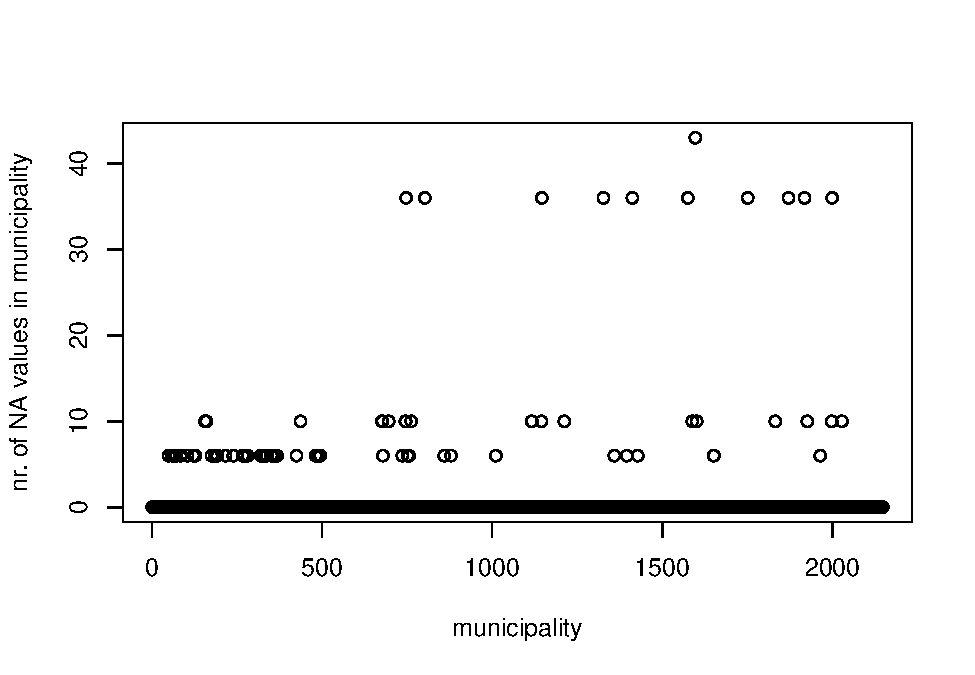
\includegraphics{Influence_factors_files/figure-latex/1.05_Multiple_missing-1.pdf}
11 observations have 36 (or more) missing values. This reflects all
columns, which show at least 11 missing values. For these specific
municipalities, it doesn't make any sense to compute the mean value.
Also for the others, there are always multiple columns with missing data
at the same time (at least 6), so these rows will be deleted. Still
enough data is there.

\begin{Shaded}
\begin{Highlighting}[]
\CommentTok{\# replace NaN values or "Inf" values with NA}
\NormalTok{d.share[}\FunctionTok{is.na}\NormalTok{(d.share) }\SpecialCharTok{|}\NormalTok{ d.share }\SpecialCharTok{==} \StringTok{"Inf"}\NormalTok{] }\OtherTok{\textless{}{-}} \ConstantTok{NA}
\NormalTok{d.count[}\FunctionTok{is.na}\NormalTok{(d.count) }\SpecialCharTok{|}\NormalTok{ d.count }\SpecialCharTok{==} \StringTok{"Inf"}\NormalTok{] }\OtherTok{\textless{}{-}} \ConstantTok{NA}

\DocumentationTok{\#\# Removing all observations with NA!}

\NormalTok{d.share }\OtherTok{\textless{}{-}} \FunctionTok{na.omit}\NormalTok{(d.share)}
\NormalTok{d.count }\OtherTok{\textless{}{-}} \FunctionTok{na.omit}\NormalTok{(d.count)}
\end{Highlighting}
\end{Shaded}

\newpage

\hypertarget{graphical-analysis}{%
\subsection{Graphical Analysis}\label{graphical-analysis}}

In this chapter, several analysis steps based on graphics will be
performed to get a meaningful insight into the data. The used methods
only cover a little part of the huge possibilities when it comes to
visualizations. I mainly focused on the ``ggplot''-package as it comes
with a wide range of options.

\hypertarget{share-data-density-plots-of-different-influence-factors}{%
\subsubsection{Share Data: Density plots of different influence
factors}\label{share-data-density-plots-of-different-influence-factors}}

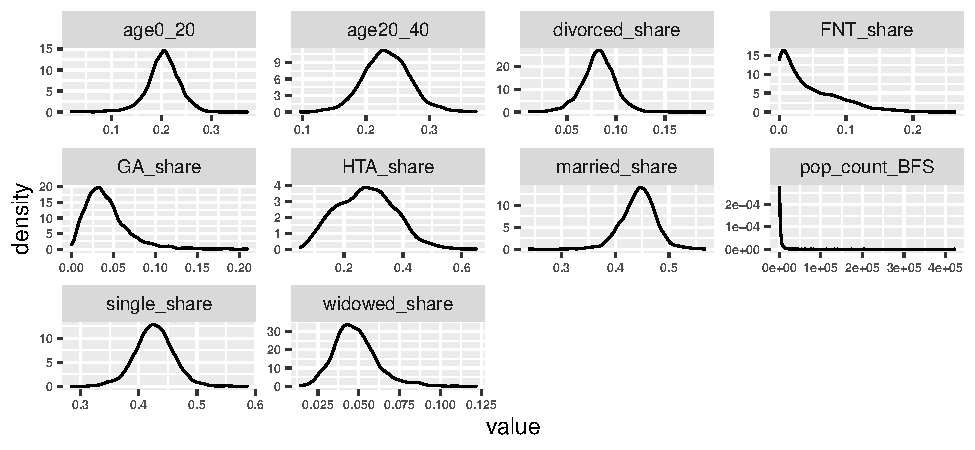
\includegraphics{Influence_factors_files/figure-latex/1.07_density_plots1-1.pdf}
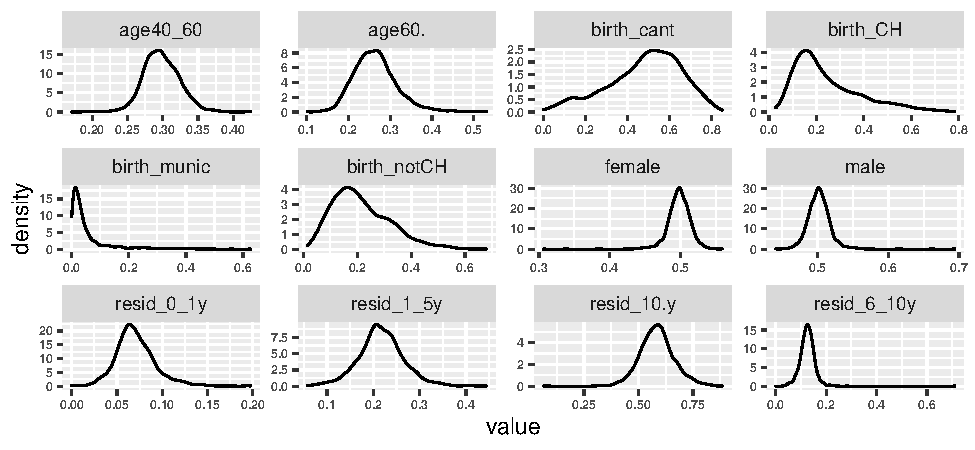
\includegraphics{Influence_factors_files/figure-latex/1.07_density_plots1-2.pdf}
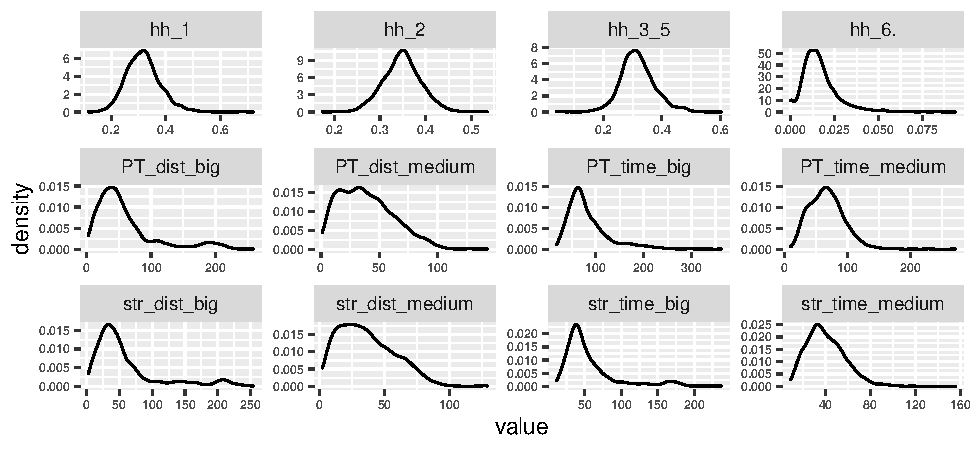
\includegraphics{Influence_factors_files/figure-latex/1.07_density_plots1-3.pdf}
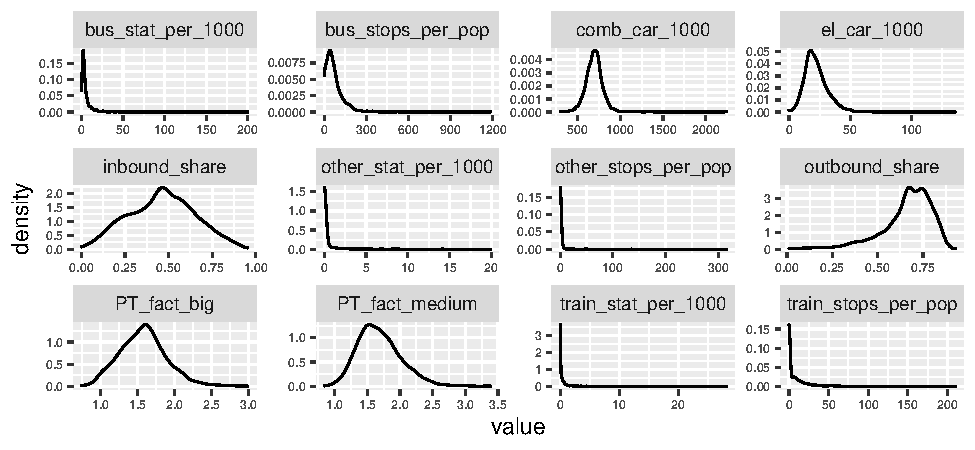
\includegraphics{Influence_factors_files/figure-latex/1.07_density_plots1-4.pdf}

\hypertarget{count-data-density-plots-of-different-influence-factors}{%
\subsubsection{Count Data: Density plots of different influence
factors}\label{count-data-density-plots-of-different-influence-factors}}

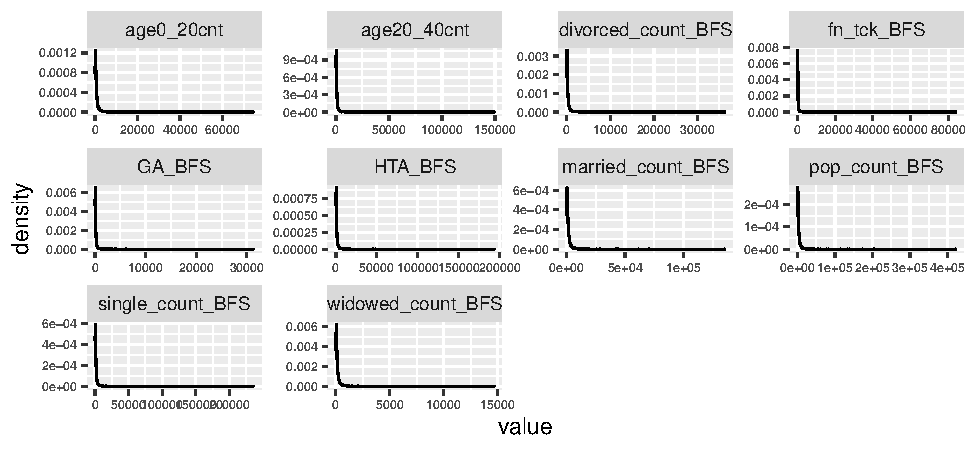
\includegraphics{Influence_factors_files/figure-latex/1.08_density_plots2-1.pdf}
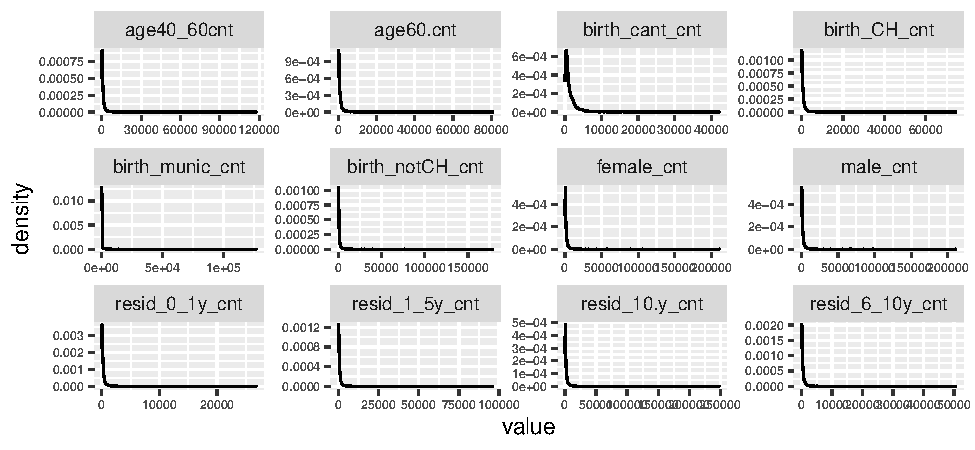
\includegraphics{Influence_factors_files/figure-latex/1.08_density_plots2-2.pdf}
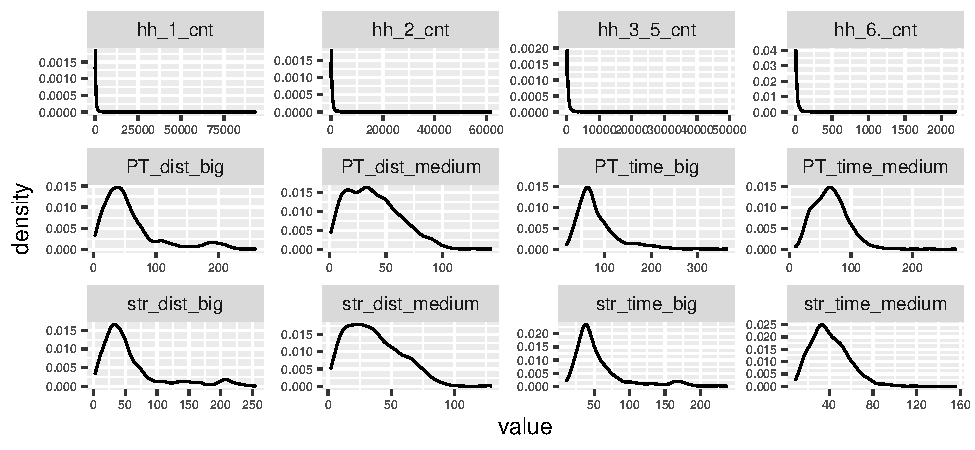
\includegraphics{Influence_factors_files/figure-latex/1.08_density_plots2-3.pdf}
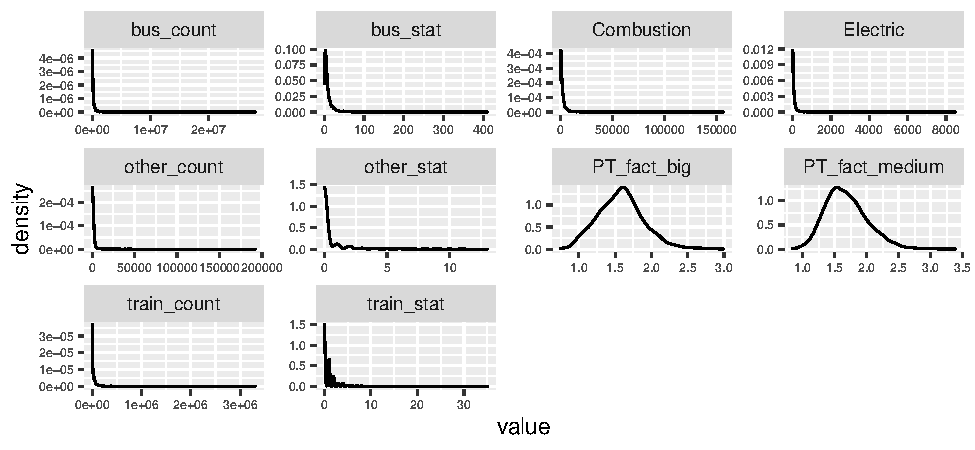
\includegraphics{Influence_factors_files/figure-latex/1.08_density_plots2-4.pdf}

All data except the PT\_fact\_big and PT\_fact\_medium are right-skewed
and have to be logarithmized to normalize!

\hypertarget{normalizing-data}{%
\subsection{Normalizing data}\label{normalizing-data}}

The normalization is important due to some outstanding variables. Due to
the different data distribution in the share and count datasets,
different approaches will be used for the two sets.

\hypertarget{normalizing-share-values}{%
\subsubsection{Normalizing Share
Values}\label{normalizing-share-values}}

In the case of the share dataset, the normalization mainly affects those
variables that have no shares, as these already lie between 0 and 1
anyway. But to standardize all continuous variables at the same scale, I
will include all parameters except the target variable into the
normalization. The `scale'-function should do the necessary
normalization in these cases.

\begin{Shaded}
\begin{Highlighting}[]
\CommentTok{\# NORMALIZING SHARE VALUES}
\NormalTok{d.norm.share }\OtherTok{\textless{}{-}}\NormalTok{ d.share[,}\DecValTok{4}\SpecialCharTok{:}\DecValTok{50}\NormalTok{]}
\CommentTok{\# print(colnames(d.norm.share))}

\CommentTok{\# define columns to normalize:}
\NormalTok{columns }\OtherTok{\textless{}{-}} \FunctionTok{c}\NormalTok{(}\StringTok{"single\_share"}\NormalTok{, }\StringTok{"married\_share"}\NormalTok{,}
             \StringTok{"widowed\_share"}\NormalTok{, }\StringTok{"divorced\_share"}\NormalTok{, }\StringTok{"age0\_20"}\NormalTok{, }\StringTok{"age20\_40"}\NormalTok{, }\StringTok{"age40\_60"}\NormalTok{, }
             \StringTok{"age60."}\NormalTok{, }\StringTok{"birth\_munic"}\NormalTok{, }\StringTok{"birth\_cant"}\NormalTok{, }\StringTok{"birth\_CH"}\NormalTok{, }\StringTok{"birth\_notCH"}\NormalTok{, }
             \StringTok{"male"}\NormalTok{, }\StringTok{"female"}\NormalTok{, }\StringTok{"resid\_0\_1y"}\NormalTok{, }\StringTok{"resid\_1\_5y"}\NormalTok{, }\StringTok{"resid\_6\_10y"}\NormalTok{, }\StringTok{"resid\_10.y"}\NormalTok{,}
             \StringTok{"hh\_1"}\NormalTok{, }\StringTok{"hh\_2"}\NormalTok{, }\StringTok{"hh\_3\_5"}\NormalTok{, }\StringTok{"hh\_6."}\NormalTok{, }\StringTok{"PT\_dist\_medium"}\NormalTok{, }\StringTok{"PT\_time\_medium"}\NormalTok{, }
             \StringTok{"PT\_dist\_big"}\NormalTok{, }\StringTok{"PT\_time\_big"}\NormalTok{, }\StringTok{"str\_dist\_medium"}\NormalTok{, }\StringTok{"str\_time\_medium"}\NormalTok{, }
             \StringTok{"str\_dist\_big"}\NormalTok{, }\StringTok{"str\_time\_big"}\NormalTok{, }\StringTok{"PT\_fact\_big"}\NormalTok{, }\StringTok{"PT\_fact\_medium"}\NormalTok{,}
             \StringTok{"bus\_stops\_per\_pop"}\NormalTok{, }\StringTok{"train\_stops\_per\_pop"}\NormalTok{, }\StringTok{"other\_stops\_per\_pop"}\NormalTok{,}
             \StringTok{"bus\_stat\_per\_1000"}\NormalTok{, }\StringTok{"train\_stat\_per\_1000"}\NormalTok{, }\StringTok{"other\_stat\_per\_1000"}\NormalTok{,}
             \StringTok{"comb\_car\_1000"}\NormalTok{, }\StringTok{"el\_car\_1000"}\NormalTok{, }\StringTok{"inbound\_share"}\NormalTok{, }\StringTok{"outbound\_share"}\NormalTok{)}

\CommentTok{\# normalize data!}
\NormalTok{d.norm.share[columns] }\OtherTok{\textless{}{-}} \FunctionTok{scale}\NormalTok{(d.norm.share[columns]) }
  \CommentTok{\# scale function: mean = 0, standard deviation = 1}
\end{Highlighting}
\end{Shaded}

The used scale function normalizes data through centering (setting mean
of each variable to 0 by subtracting the mean value of all observations)
and scaling (setting standard deviation to 1 by dividing all
observations to the standard deviation of the column). The values
achieved in this way all have the same weight in relation to a model.
Thus, the resulting parameters can be compared with each other later on.

\hypertarget{normalizing-count-data}{%
\subsubsection{Normalizing Count data}\label{normalizing-count-data}}

As observed in chapter 1.4.2, most count data have a right-skewed
distribution and should therefore be log-transformed. The only variables
this hardly affects are ``PT\_fact\_big'' and ``PT\_fact\_medium'',
which have an approximate normal distribution. For this reason, these
variables are not taken into account in the normalization.

\begin{Shaded}
\begin{Highlighting}[]
\CommentTok{\# NORMALIZING COUNT DATA}

\CommentTok{\# log{-}transform all columns except PT\_fact\_big, PT\_fact\_medium and language}
\NormalTok{d.norm.count }\OtherTok{\textless{}{-}} \FunctionTok{log}\NormalTok{(d.count[, }\SpecialCharTok{!}\FunctionTok{names}\NormalTok{(d.count) }
                            \SpecialCharTok{\%in\%} \FunctionTok{c}\NormalTok{(}\StringTok{"language"}\NormalTok{, }\StringTok{"PT\_fact\_big"}\NormalTok{, }\StringTok{"PT\_fact\_medium"}\NormalTok{,}
                                  \StringTok{"BFS\_Nr"}\NormalTok{, }\StringTok{"municipality"}\NormalTok{, }\StringTok{"canton"}\NormalTok{)]}\SpecialCharTok{+}\DecValTok{1}\NormalTok{) }
                                    \CommentTok{\# \textquotesingle{}+1\textquotesingle{} due to log(0) = {-}Inf!}

\CommentTok{\# add the 3 deleted columns again!}
\NormalTok{d.norm.count[}\StringTok{"language"}\NormalTok{] }\OtherTok{\textless{}{-}}\NormalTok{ d.count[}\StringTok{"language"}\NormalTok{]}
\NormalTok{d.norm.count[}\StringTok{"PT\_fact\_big"}\NormalTok{] }\OtherTok{\textless{}{-}}\NormalTok{ d.count[}\StringTok{"PT\_fact\_big"}\NormalTok{]}
\NormalTok{d.norm.count[}\StringTok{"PT\_fact\_medium"}\NormalTok{] }\OtherTok{\textless{}{-}}\NormalTok{ d.count[}\StringTok{"PT\_fact\_medium"}\NormalTok{]}
\end{Highlighting}
\end{Shaded}

\newpage

\hypertarget{ga-hta-fnt-shares-compared-to-languages}{%
\subsection{GA, HTA \& FNT shares compared to
languages:}\label{ga-hta-fnt-shares-compared-to-languages}}

A first insight can be gained by comparing the different target share
values (HTA, GA, FNT) with the language regions as the only categorical
variable present:

\begin{Shaded}
\begin{Highlighting}[]
\NormalTok{plot\_HTA }\OtherTok{\textless{}{-}} \FunctionTok{ggbarplot}\NormalTok{(d.share, }\AttributeTok{x=}\StringTok{"language"}\NormalTok{, }\AttributeTok{y=}\StringTok{"HTA\_share"}\NormalTok{, }\AttributeTok{fill=}\StringTok{"language"}\NormalTok{,  }
                      \AttributeTok{add =} \StringTok{"mean\_se"}\NormalTok{, }\AttributeTok{xlab =} \StringTok{"language"}\NormalTok{, }\AttributeTok{legend =} \StringTok{"right"}\NormalTok{,}
                      \AttributeTok{title =} \StringTok{"HTA"}\NormalTok{, }\AttributeTok{ggtheme =} \FunctionTok{theme\_cleveland}\NormalTok{()) }\SpecialCharTok{+} \CommentTok{\# better looking}
  \FunctionTok{theme}\NormalTok{(}\AttributeTok{axis.text=}\FunctionTok{element\_text}\NormalTok{(}\AttributeTok{size=}\FloatTok{6.5}\NormalTok{, }\AttributeTok{face=}\StringTok{"bold"}\NormalTok{))}

\NormalTok{plot\_GA }\OtherTok{\textless{}{-}} \FunctionTok{ggbarplot}\NormalTok{(d.share, }\AttributeTok{x=}\StringTok{"language"}\NormalTok{, }\AttributeTok{y=}\StringTok{"GA\_share"}\NormalTok{, }\AttributeTok{fill=}\StringTok{"language"}\NormalTok{, }\AttributeTok{add =} \StringTok{"mean\_se"}\NormalTok{,}
                      \AttributeTok{xlab =} \StringTok{"language"}\NormalTok{, }\AttributeTok{legend =} \StringTok{"right"}\NormalTok{, }
                     \AttributeTok{title =} \StringTok{"GA"}\NormalTok{, }\AttributeTok{ggtheme =} \FunctionTok{theme\_cleveland}\NormalTok{()) }\SpecialCharTok{+}
  \FunctionTok{theme}\NormalTok{(}\AttributeTok{axis.text=}\FunctionTok{element\_text}\NormalTok{(}\AttributeTok{size=}\FloatTok{6.5}\NormalTok{, }\AttributeTok{face=}\StringTok{"bold"}\NormalTok{))}

\NormalTok{plot\_FNT }\OtherTok{\textless{}{-}} \FunctionTok{ggbarplot}\NormalTok{(d.share, }\AttributeTok{x=}\StringTok{"language"}\NormalTok{, }\AttributeTok{y=}\StringTok{"FNT\_share"}\NormalTok{, }\AttributeTok{fill=}\StringTok{"language"}\NormalTok{, }
                      \AttributeTok{add =} \StringTok{"mean\_se"}\NormalTok{, }\AttributeTok{xlab =} \StringTok{"language"}\NormalTok{, }\AttributeTok{legend =} \StringTok{"right"}\NormalTok{,}
                      \AttributeTok{title =} \StringTok{"FNT"}\NormalTok{, }\AttributeTok{ggtheme =} \FunctionTok{theme\_cleveland}\NormalTok{()) }\SpecialCharTok{+}
  \FunctionTok{theme}\NormalTok{(}\AttributeTok{axis.text=}\FunctionTok{element\_text}\NormalTok{(}\AttributeTok{size=}\FloatTok{6.5}\NormalTok{, }\AttributeTok{face=}\StringTok{"bold"}\NormalTok{))}

\NormalTok{share.comparison }\OtherTok{\textless{}{-}} \FunctionTok{ggarrange}\NormalTok{(plot\_GA, plot\_HTA, plot\_FNT, }\AttributeTok{ncol=}\DecValTok{3}\NormalTok{) }\CommentTok{\# 3 plots beside each other}

\FunctionTok{annotate\_figure}\NormalTok{(share.comparison, }
    \AttributeTok{top =} \FunctionTok{text\_grob}\NormalTok{(}\StringTok{"Comparison of mean share of GA, HTA and FNT sold in \% of population"}\NormalTok{, }
                                \AttributeTok{face =} \StringTok{"bold"}\NormalTok{)) }\CommentTok{\# set over{-}all title ("top")}
\end{Highlighting}
\end{Shaded}

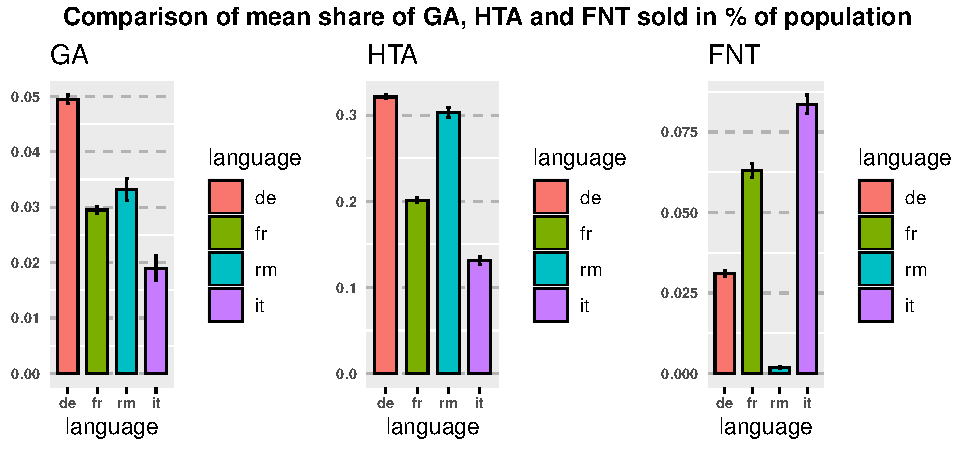
\includegraphics{Influence_factors_files/figure-latex/1.11_language_shares-1.pdf}
Interesting insights can be gained here: For the GA tickets, the share
is highest in the German municipalities and lowest in the Italian
regions. The rate in the German-speaking region is thereby 2.5 times as
high as in Ticino. The picture is similar for the Half-Fare Card (HTA),
with shares generally in much higher percentage ranges. The relatively
high proportion in Rhaeto-Romanic speaking municipalities is remarkable,
which is about the same as in German-speaking Switzerland.

A completely different picture emerges for the fare network tickets
(FNT). Now, the non-German-speaking areas, led by Ticino with just under
8\%, have the highest share of fare network tickets. The rate in
French-speaking Switzerland is also not much lower at around 6\%, while
German-speaking Switzerland only achieves a share of 3\%.

\newpage

\hypertarget{modelling-shares}{%
\section{MODELLING SHARES}\label{modelling-shares}}

I will achieve the first objective of modelling the share of season
tickets through two different approaches: Linear model (LM) and
generalized linear model (GLM) with family ``binomial''.

\hypertarget{parameter-selection}{%
\subsection{Parameter selection}\label{parameter-selection}}

Before starting with the models, the amount of possible influence
factors must be reduced. Still many parameters are present, which
strongly rely on each other, for example the different PT / Street
distance + time tables:

\hypertarget{street-and-pt-distance-time-tables}{%
\subsubsection{street and PT distance + time
tables:}\label{street-and-pt-distance-time-tables}}

\begin{Shaded}
\begin{Highlighting}[]
\FunctionTok{chart.Correlation}\NormalTok{(d.norm.count[,}\FunctionTok{c}\NormalTok{(}\DecValTok{27}\SpecialCharTok{:}\DecValTok{34}\NormalTok{, }\DecValTok{44}\SpecialCharTok{:}\DecValTok{45}\NormalTok{)], }\CommentTok{\# +1 due to 0{-}values (log(0) = {-}Inf)}
                  \AttributeTok{histogram=}\ConstantTok{TRUE}\NormalTok{) }\CommentTok{\# adding histograms to the plot}
\end{Highlighting}
\end{Shaded}

\includegraphics{Influence_factors_files/figure-latex/2.01_corr_charts-1.pdf}
Many correlation values are strongly significant, the collinearity is
huge in these cases! There has to be done something here. The distance
and time data are always strongly correlating for big and medium cities,
so I will focus only on time data. Within the same city category, PT and
str data are additionnally also correlating highly, so only the PT data
is used. The PT factor will be used as well, the correlation values are
not that high, even if one of the inputs for the calculation are the
PT\_time\_big and PT\_time\_medium tables. Decision: For further uses,
the following variables will be used:

\begin{itemize}
\tightlist
\item
  PT\_fact\_big
\item
  PT\_fact\_medium
\item
  PT\_time\_big
\item
  PT\_time\_medium
\end{itemize}

\begin{Shaded}
\begin{Highlighting}[]
\CommentTok{\# remove undesired columns \#1 from COUNT DATA}
\NormalTok{d.norm.count }\OtherTok{\textless{}{-}}\NormalTok{ d.norm.count[, }\SpecialCharTok{!}\FunctionTok{names}\NormalTok{(d.norm.count) }\CommentTok{\# remove the following columns:}
                             \SpecialCharTok{\%in\%} \FunctionTok{c}\NormalTok{(}\StringTok{"PT\_dist\_medium"}\NormalTok{, }\StringTok{"PT\_dist\_big"}\NormalTok{, }\StringTok{"str\_dist\_medium"}\NormalTok{, }
                                    \StringTok{"str\_time\_medium"}\NormalTok{, }\StringTok{"str\_dist\_big"}\NormalTok{, }\StringTok{"str\_time\_big"}\NormalTok{)]}

\CommentTok{\# remove undesired columns \#1 from SHARE DATA}
\NormalTok{d.norm.share }\OtherTok{\textless{}{-}}\NormalTok{ d.norm.share[, }\SpecialCharTok{!}\FunctionTok{names}\NormalTok{(d.norm.share) }\CommentTok{\# remove the following columns:}
                             \SpecialCharTok{\%in\%} \FunctionTok{c}\NormalTok{(}\StringTok{"PT\_dist\_medium"}\NormalTok{, }\StringTok{"PT\_dist\_big"}\NormalTok{, }\StringTok{"str\_dist\_medium"}\NormalTok{, }
                                    \StringTok{"str\_time\_medium"}\NormalTok{, }\StringTok{"str\_dist\_big"}\NormalTok{, }\StringTok{"str\_time\_big"}\NormalTok{)]}
\end{Highlighting}
\end{Shaded}

\hypertarget{categorical-data}{%
\subsubsection{Categorical data}\label{categorical-data}}

Furthermore, many original categorical data (personal data) has been
used to show demographic structure (age segments, household size etc.).
With the given population data (pop\_count\_BFS) and the categories male
and female for example, the number of male explains the number of
females in the municipality (population - male). For each of this
categories, one can be removed. This affects the following variables,
which are removed:

\begin{itemize}
\tightlist
\item
  divorced\_count\_BFS
\item
  age60.cnt
\item
  birth\_notCH\_cnt
\item
  female\_cnt
\item
  resid\_10.y\_cnt
\item
  hh6.\_cnt
\end{itemize}

The same procedure can also be used for the share data set, since, for
example, the proportion of men in a municipality simultaneously explains
the proportion of women.

\begin{Shaded}
\begin{Highlighting}[]
\CommentTok{\# remove undesired columns \#2 SHARE DATA}
\NormalTok{d.norm.count }\OtherTok{\textless{}{-}}\NormalTok{ d.norm.count[, }\SpecialCharTok{!}\FunctionTok{names}\NormalTok{(d.norm.count) }\CommentTok{\# remove the following columns:}
                             \SpecialCharTok{\%in\%} \FunctionTok{c}\NormalTok{(}\StringTok{"divorced\_count\_BFS"}\NormalTok{, }\StringTok{"age60.cnt"}\NormalTok{, }\StringTok{"birth\_notCH\_cnt"}\NormalTok{, }
                                    \StringTok{"female\_cnt"}\NormalTok{, }\StringTok{"resid\_10.y\_cnt"}\NormalTok{, }\StringTok{"hh\_6.\_cnt"}\NormalTok{)]}

\CommentTok{\# remove undesired columns \#2 COUNT DATA}
\NormalTok{d.norm.share }\OtherTok{\textless{}{-}}\NormalTok{ d.norm.share[, }\SpecialCharTok{!}\FunctionTok{names}\NormalTok{(d.norm.share) }\CommentTok{\# remove the following columns: }
                             \SpecialCharTok{\%in\%} \FunctionTok{c}\NormalTok{(}\StringTok{"divorced\_share"}\NormalTok{, }\StringTok{"age60."}\NormalTok{, }\StringTok{"birth\_notCH"}\NormalTok{, }
                                    \StringTok{"female"}\NormalTok{, }\StringTok{"resid\_10.y"}\NormalTok{, }\StringTok{"hh\_6."}\NormalTok{)]}
\end{Highlighting}
\end{Shaded}

\hypertarget{train-test-splitting-sharecount-datasets-original-normalized-each}{%
\subsection{Train / Test splitting Share/count datasets (original +
normalized
each)}\label{train-test-splitting-sharecount-datasets-original-normalized-each}}

With the selection of data complete, the data set can now be split into
a training and test set. This is important in modelling to detect
potential overfitting if the accuracy of the model is much higher for
the training set than for the test data. Splitting is done for all data
sets that will be used later in the modelling, i.e.~the normalised count
and share data:

\hypertarget{normalized-share-dataset}{%
\subsubsection{Normalized share
dataset}\label{normalized-share-dataset}}

\begin{Shaded}
\begin{Highlighting}[]
\FunctionTok{set.seed}\NormalTok{(}\DecValTok{234}\NormalTok{) }\CommentTok{\# reproducible}
\NormalTok{indexes }\OtherTok{\textless{}{-}} \FunctionTok{createDataPartition}\NormalTok{(d.norm.share}\SpecialCharTok{$}\NormalTok{pop\_count\_BFS, }\AttributeTok{p =}\NormalTok{ .}\DecValTok{8}\NormalTok{, }\AttributeTok{list =} \ConstantTok{FALSE}\NormalTok{) }
\NormalTok{d.norm.share.train }\OtherTok{\textless{}{-}}\NormalTok{ d.norm.share[indexes, ]}
\NormalTok{d.norm.share.test }\OtherTok{\textless{}{-}}\NormalTok{ d.norm.share[}\SpecialCharTok{{-}}\NormalTok{indexes, ]}
\end{Highlighting}
\end{Shaded}

\hypertarget{normalized-count-dataset}{%
\subsubsection{Normalized count
dataset}\label{normalized-count-dataset}}

\begin{Shaded}
\begin{Highlighting}[]
\FunctionTok{set.seed}\NormalTok{(}\DecValTok{234}\NormalTok{) }\CommentTok{\# reproducible}
\NormalTok{indexes }\OtherTok{\textless{}{-}} \FunctionTok{createDataPartition}\NormalTok{(d.norm.count}\SpecialCharTok{$}\NormalTok{pop\_count\_BFS, }\AttributeTok{p =}\NormalTok{ .}\DecValTok{8}\NormalTok{, }\AttributeTok{list =} \ConstantTok{FALSE}\NormalTok{) }
\NormalTok{d.norm.count.train }\OtherTok{\textless{}{-}}\NormalTok{ d.norm.count[indexes, ]}
\NormalTok{d.norm.count.test }\OtherTok{\textless{}{-}}\NormalTok{ d.norm.count[}\SpecialCharTok{{-}}\NormalTok{indexes, ]}
\end{Highlighting}
\end{Shaded}

\hypertarget{modelling-general-season-tickets-ga}{%
\subsection{Modelling General Season tickets
(GA)}\label{modelling-general-season-tickets-ga}}

This analysis starts with the first target variable, the GA. The share
as well as the count will be calculated in the following chapter using
two methods, the Generalized Linear Model with family Binomial and the
Linear Model.

\hypertarget{generalized-linear-model-glm-with-family-binomial-ga}{%
\subsubsection{Generalized Linear model (GLM) with family ``Binomial''
(GA)}\label{generalized-linear-model-glm-with-family-binomial-ga}}

With a linear model, no probability distributions can be predicted, as
values above 1 and below 0 are possible, resulting in meaningless values
concerning the share. Therefore, a logistic approach comes into play,
which strictly forecasts values between 0 and 1. Although I do not have
values for individuals with regard to the share and thus do not model a
binary target variable, a \emph{multinomial logit model approach is
described for aggregated data using group variable, which is in my case
the municipality (Morais et al., 2016).} \emph{Quasibinomial glm
fulfills the criteria here:}

\hypertarget{binomial-vs.-quasibinomial}{%
\paragraph{\texorpdfstring{Binomial
vs.~quasibinomial\newline}{Binomial vs.~quasibinomial}}\label{binomial-vs.-quasibinomial}}

There are several options when choosing the option ``family'' in the
GLM. By default, ``binomial'' is used for a binomial model. In cases
where the dispersion is too large or too small (over- and
underdispersion), a ``quasibinomial'' model can be used, which has an
additional dispersion parameter. This helps to ensure that significances
can be detected. \emph{According to the literature, the model is used
when \ldots{}} For these reasons, a quasibinomial model is also used
here. The disadvantage here is that no stepwise procedure for paremeter
elimination can be applied, as this is not permitted by the definition
of the model.

\hypertarget{glm-model-runs-ga}{%
\paragraph{\texorpdfstring{GLM model runs
(GA)\newline}{GLM model runs (GA)}}\label{glm-model-runs-ga}}

The first run is done by using all possible influence factors except the
two remaining target variables:

\begin{Shaded}
\begin{Highlighting}[]
\DocumentationTok{\#\#\#\#\#  Modelling GLM with share data:}

\DocumentationTok{\#\#\#\#\#\#\#\#\#\#\#\#\#\#\#\#\#\#\# Model set up 01 \#\#\#\#\#\#\#\#\#\#\#\#\#\#\#\#\#\#\#\#\#\#}
\NormalTok{glm.share}\FloatTok{.01} \OtherTok{\textless{}{-}} \FunctionTok{glm}\NormalTok{(GA\_share }\SpecialCharTok{\textasciitilde{}}\NormalTok{ (. }\SpecialCharTok{{-}}\NormalTok{ HTA\_share }\SpecialCharTok{{-}}\NormalTok{ FNT\_share)}\SpecialCharTok{\^{}}\DecValTok{2}\NormalTok{, }\CommentTok{\# all interactions included!}
                \AttributeTok{family =}\NormalTok{ quasibinomial, }\AttributeTok{data=}\NormalTok{d.norm.share)}

\FunctionTok{summary}\NormalTok{(glm.share}\FloatTok{.01}\NormalTok{) }
\DocumentationTok{\#\#\# Summary output not printed, due to all possible interactions shown}
\end{Highlighting}
\end{Shaded}

Starting from the output of the first experiment, all possible
interactions outside the script were examined and all those that were
classified as relevant were included in the second experiment, while all
other interactions were no longer present:

\begin{Shaded}
\begin{Highlighting}[]
\DocumentationTok{\#\#\#\#\#\#\#\# Including interaction (see excel sheet)}
\NormalTok{glm.share}\FloatTok{.02} \OtherTok{\textless{}{-}} \FunctionTok{glm}\NormalTok{(GA\_share }\SpecialCharTok{\textasciitilde{}}\NormalTok{ . }\SpecialCharTok{{-}}\NormalTok{ HTA\_share }\SpecialCharTok{{-}}\NormalTok{ FNT\_share}
                    \SpecialCharTok{+}\NormalTok{ bus\_stops\_per\_pop}\SpecialCharTok{:}\NormalTok{bus\_stat\_per\_1000}
                    \SpecialCharTok{+}\NormalTok{ train\_stops\_per\_pop}\SpecialCharTok{:}\NormalTok{train\_stat\_per\_1000}
                    \SpecialCharTok{+}\NormalTok{ other\_stops\_per\_pop}\SpecialCharTok{:}\NormalTok{other\_stops\_per\_pop}
                    \SpecialCharTok{+}\NormalTok{ PT\_fact\_big}\SpecialCharTok{:}\NormalTok{PT\_fact\_medium}
                    \SpecialCharTok{+}\NormalTok{ PT\_time\_big}\SpecialCharTok{:}\NormalTok{PT\_fact\_big}
                    \SpecialCharTok{+}\NormalTok{ PT\_time\_medium}\SpecialCharTok{:}\NormalTok{PT\_time\_big}
                    \SpecialCharTok{+}\NormalTok{ PT\_fact\_medium}\SpecialCharTok{:}\NormalTok{PT\_time\_medium, }
                \AttributeTok{family =}\NormalTok{ binomial, }\AttributeTok{data=}\NormalTok{d.norm.share) }
    \DocumentationTok{\#\# binomial model as a try for further stepwise selection!}
\FunctionTok{summary}\NormalTok{(glm.share}\FloatTok{.02}\NormalTok{)}
\end{Highlighting}
\end{Shaded}

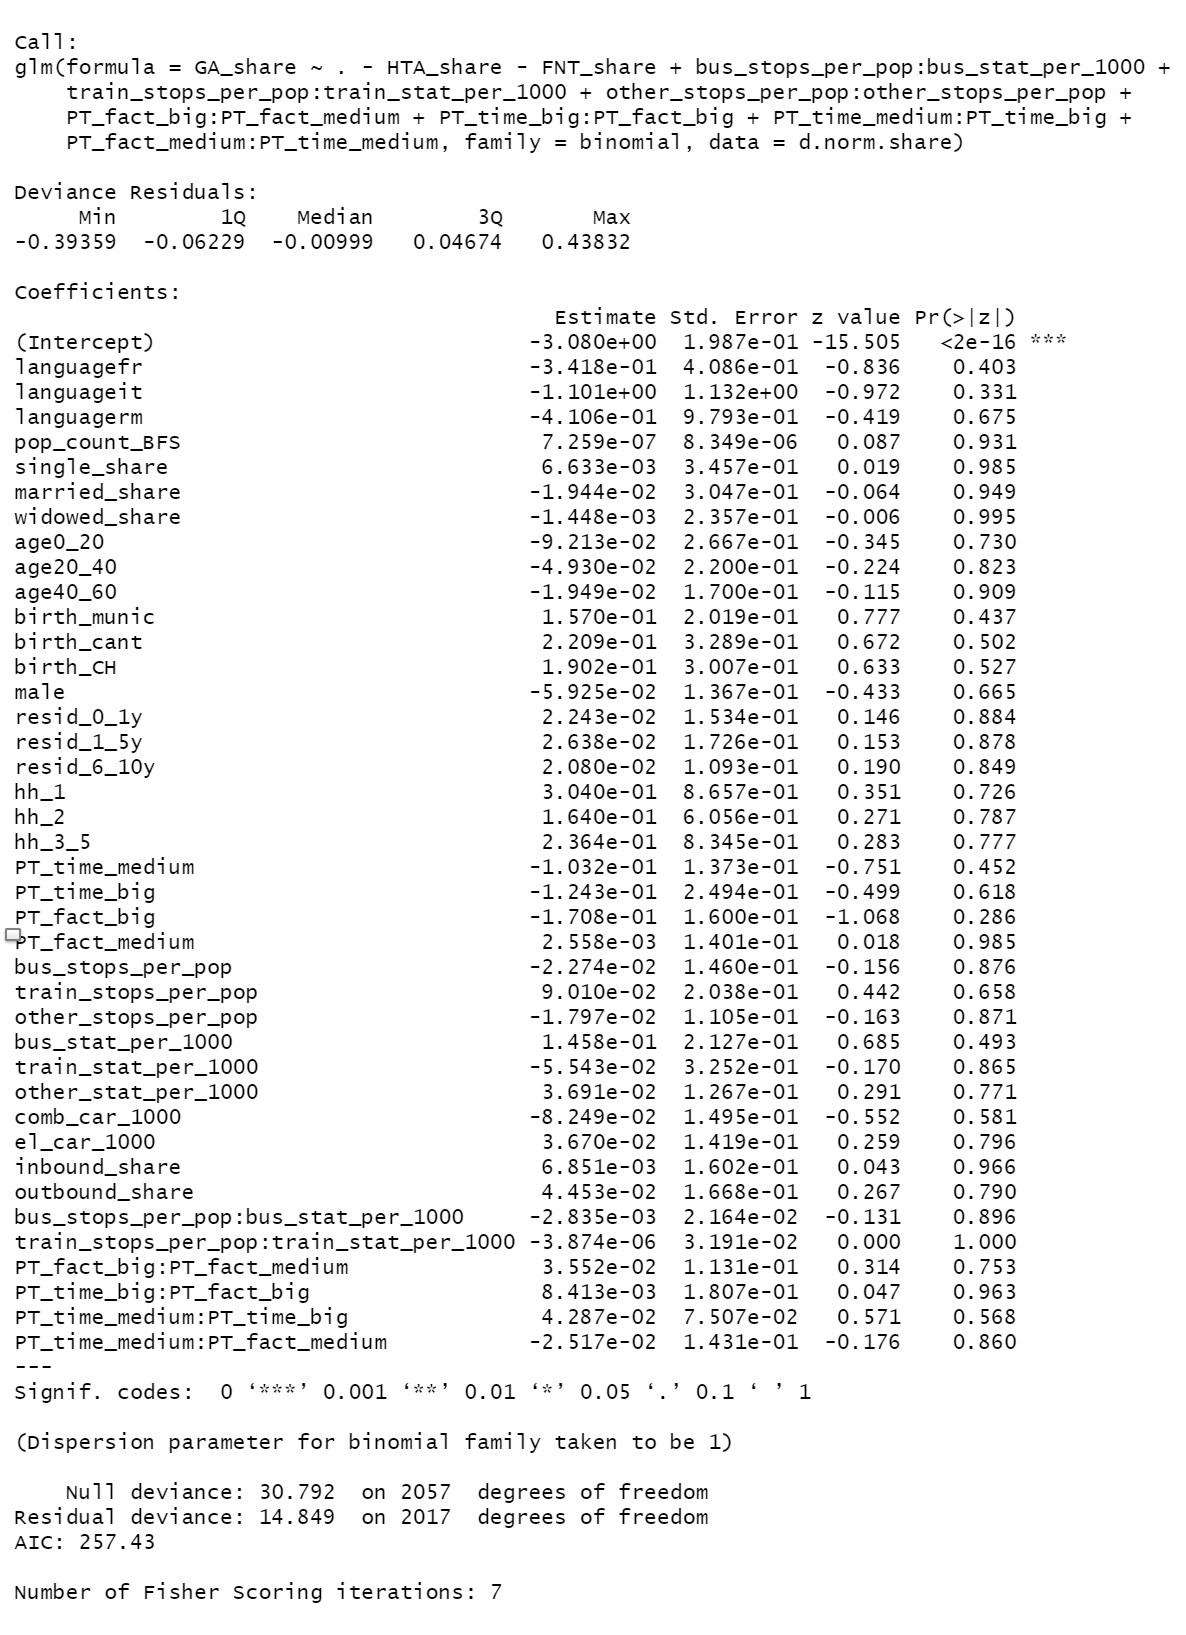
\includegraphics{GLM_share_02_summary.png}

Now a model with the family ``binomial'' was used. It is relatively
quickly apparent that no parameter is considered significant. However,
in principle, a stepwise procedure for parameter selection is possible
in this way, which is applied in the next step:

\begin{Shaded}
\begin{Highlighting}[]
\DocumentationTok{\#\#\#\#\#\#\#\#\#\#\#\#\#\#\# Stepwise parameter selection forward and backwards!\#\#\#\#\#\#\#\#\#\#\#}
\NormalTok{glm.share}\FloatTok{.03} \OtherTok{\textless{}{-}} \FunctionTok{stepAIC}\NormalTok{(glm.share}\FloatTok{.02}\NormalTok{, }\AttributeTok{direction=}\StringTok{"both"}\NormalTok{, }\AttributeTok{trace=}\ConstantTok{FALSE}\NormalTok{)}

\FunctionTok{summary}\NormalTok{(glm.share}\FloatTok{.03}\NormalTok{)}
\end{Highlighting}
\end{Shaded}

\begin{verbatim}
## 
## Call:
## glm(formula = GA_share ~ age0_20 + PT_time_big + PT_fact_big, 
##     family = binomial, data = d.norm.share)
## 
## Deviance Residuals: 
##      Min        1Q    Median        3Q       Max  
## -0.29242  -0.07647  -0.01404   0.05599   0.53501  
## 
## Coefficients:
##             Estimate Std. Error z value Pr(>|z|)    
## (Intercept)  -3.1860     0.1156 -27.560   <2e-16 ***
## age0_20      -0.2025     0.1266  -1.600   0.1096    
## PT_time_big  -0.2456     0.1300  -1.889   0.0589 .  
## PT_fact_big  -0.2013     0.1214  -1.659   0.0971 .  
## ---
## Signif. codes:  0 '***' 0.001 '**' 0.01 '*' 0.05 '.' 0.1 ' ' 1
## 
## (Dispersion parameter for binomial family taken to be 1)
## 
##     Null deviance: 30.792  on 2057  degrees of freedom
## Residual deviance: 22.629  on 2054  degrees of freedom
## AIC: 183.04
## 
## Number of Fisher Scoring iterations: 6
\end{verbatim}

Doing this, the process stops very late, having only age0\_20,
PT\_fact\_big and PT\_time\_big left. The problem here comes from the
above discussed problem of the overdispersion when using the binomial
model.

The quasibinomial model on one side shows significances of parameters,
but does not allow a stepwise variable selection with stepAIC function.
The RMSE and R square values are on the other hand exactly the same,
showing identic prediction behaviour. Therefore, the quasibinomial model
can be used to selected parameters for a further try for the GLM. One
possibility is still an option: The parameter selection can be done by
taking the significant parameters from ta linear model approach, having
the assumption that the same parameters are relevant for a linear model
as for a GLM with the family binomial or quasibinomial. Therefore, a
linear model is now built first before the analysis of the GLM can go
further.

\hypertarget{linear-model-lm-ga}{%
\subsubsection{Linear Model (LM) (GA)}\label{linear-model-lm-ga}}

Now, a linear model is built, which models the absolute numbers of GA's
per municipality. Due to the restriction of a linear model, it is not
possible to model shares in a population with a linear model, as for a
linear model, also negative values and values above 1 can occur which
contradicts the possible range of the target variable. Therefore, the
count dataset is used here. As is the case with the share dataset, all
values except the target variable are normalized in the count data.

The main goal of the linear model is to gain insights into the automatic
parameter selection when applying a stepwise AIC-selection approach.
This can be used afterwards for the GLM again.

\begin{Shaded}
\begin{Highlighting}[]
\CommentTok{\# First model with all predictors including defined interaction terms:}
\NormalTok{lm.count}\FloatTok{.01} \OtherTok{\textless{}{-}} \FunctionTok{lm}\NormalTok{(GA\_BFS }\SpecialCharTok{\textasciitilde{}}\NormalTok{ . }\SpecialCharTok{{-}}\NormalTok{HTA\_BFS }\SpecialCharTok{{-}}\NormalTok{ fn\_tck\_BFS }
                    \SpecialCharTok{+}\NormalTok{ bus\_count}\SpecialCharTok{:}\NormalTok{bus\_stat}
                    \SpecialCharTok{+}\NormalTok{ train\_count}\SpecialCharTok{:}\NormalTok{train\_stat}
                    \SpecialCharTok{+}\NormalTok{ other\_count}\SpecialCharTok{:}\NormalTok{other\_stat}
                    \SpecialCharTok{+}\NormalTok{ PT\_fact\_big}\SpecialCharTok{:}\NormalTok{PT\_fact\_medium}
                    \SpecialCharTok{+}\NormalTok{ PT\_time\_big}\SpecialCharTok{:}\NormalTok{PT\_fact\_big}
                    \SpecialCharTok{+}\NormalTok{ PT\_time\_medium}\SpecialCharTok{:}\NormalTok{PT\_time\_big}
                    \SpecialCharTok{+}\NormalTok{ PT\_fact\_medium}\SpecialCharTok{:}\NormalTok{PT\_time\_medium,}
                  \AttributeTok{data =}\NormalTok{ d.norm.count.train)}

\FunctionTok{summary}\NormalTok{(lm.count}\FloatTok{.01}\NormalTok{) }\DocumentationTok{\#\# looks generally good}
\end{Highlighting}
\end{Shaded}

\begin{verbatim}
## 
## Call:
## lm(formula = GA_BFS ~ . - HTA_BFS - fn_tck_BFS + bus_count:bus_stat + 
##     train_count:train_stat + other_count:other_stat + PT_fact_big:PT_fact_medium + 
##     PT_time_big:PT_fact_big + PT_time_medium:PT_time_big + PT_fact_medium:PT_time_medium, 
##     data = d.norm.count.train)
## 
## Residuals:
##      Min       1Q   Median       3Q      Max 
## -2.41489 -0.25064  0.03564  0.28920  2.24066 
## 
## Coefficients:
##                                Estimate Std. Error t value Pr(>|t|)    
## (Intercept)                    6.935364   1.596205   4.345 1.48e-05 ***
## pop_count_BFS                  0.974372   0.882191   1.104  0.26955    
## single_count_BFS               0.465120   0.432107   1.076  0.28191    
## married_count_BFS             -0.122698   0.412669  -0.297  0.76625    
## widowed_count_BFS             -0.072389   0.080456  -0.900  0.36840    
## age0_20cnt                    -0.376662   0.121317  -3.105  0.00194 ** 
## age20_40cnt                   -0.392180   0.132593  -2.958  0.00314 ** 
## age40_60cnt                   -0.518610   0.182295  -2.845  0.00450 ** 
## birth_munic_cnt                0.091743   0.014283   6.423 1.75e-10 ***
## birth_cant_cnt                 0.171636   0.033092   5.187 2.41e-07 ***
## birth_CH_cnt                   0.176513   0.031729   5.563 3.10e-08 ***
## male_cnt                      -0.976535   0.312777  -3.122  0.00183 ** 
## resid_0_1y_cnt                 0.056169   0.044248   1.269  0.20448    
## resid_1_5y_cnt                -0.030236   0.066738  -0.453  0.65057    
## resid_6_10y_cnt                0.163556   0.053432   3.061  0.00224 ** 
## hh_1_cnt                       0.376674   0.083306   4.522 6.59e-06 ***
## hh_2_cnt                       0.633354   0.123804   5.116 3.50e-07 ***
## hh_3_5_cnt                     0.806233   0.181431   4.444 9.45e-06 ***
## PT_time_medium                -1.137606   0.268313  -4.240 2.36e-05 ***
## PT_time_big                   -1.382030   0.247884  -5.575 2.89e-08 ***
## bus_count                     -0.014350   0.007381  -1.944  0.05203 .  
## other_count                    0.024251   0.011061   2.192  0.02849 *  
## train_count                    0.015947   0.006299   2.532  0.01145 *  
## bus_stat                       0.008816   0.079519   0.111  0.91174    
## other_stat                    -0.317758   0.173837  -1.828  0.06775 .  
## train_stat                    -0.288109   0.236471  -1.218  0.22326    
## Combustion                    -0.657271   0.094394  -6.963 4.84e-12 ***
## Electric                       0.076963   0.034421   2.236  0.02549 *  
## languagefr                    -0.367450   0.039966  -9.194  < 2e-16 ***
## languageit                    -1.177570   0.085592 -13.758  < 2e-16 ***
## languagerm                    -0.495890   0.083023  -5.973 2.86e-09 ***
## PT_fact_big                   -0.763953   0.454947  -1.679  0.09331 .  
## PT_fact_medium                 0.517505   0.355054   1.458  0.14516    
## bus_count:bus_stat             0.004921   0.005533   0.889  0.37394    
## train_count:train_stat         0.024200   0.018400   1.315  0.18863    
## other_count:other_stat         0.018868   0.017930   1.052  0.29282    
## PT_fact_big:PT_fact_medium     0.285187   0.099452   2.868  0.00419 ** 
## PT_time_big:PT_fact_big       -0.034814   0.097689  -0.356  0.72160    
## PT_time_medium:PT_time_big     0.307423   0.051634   5.954 3.21e-09 ***
## PT_time_medium:PT_fact_medium -0.227370   0.088454  -2.571  0.01024 *  
## ---
## Signif. codes:  0 '***' 0.001 '**' 0.01 '*' 0.05 '.' 0.1 ' ' 1
## 
## Residual standard error: 0.444 on 1608 degrees of freedom
## Multiple R-squared:  0.8999, Adjusted R-squared:  0.8975 
## F-statistic: 370.8 on 39 and 1608 DF,  p-value: < 2.2e-16
\end{verbatim}

The output looks good in general, but to reduce the number of
parameters, a stepwise selection model is applied:

\begin{Shaded}
\begin{Highlighting}[]
\NormalTok{lm.count}\FloatTok{.02} \OtherTok{\textless{}{-}}\NormalTok{ MASS}\SpecialCharTok{::}\FunctionTok{stepAIC}\NormalTok{(lm.count}\FloatTok{.01}\NormalTok{, }\AttributeTok{direction =} \StringTok{"both"}\NormalTok{, }\AttributeTok{trace =} \ConstantTok{FALSE}\NormalTok{)}
\FunctionTok{summary}\NormalTok{(lm.count}\FloatTok{.02}\NormalTok{)}
\end{Highlighting}
\end{Shaded}

\begin{verbatim}
## 
## Call:
## lm(formula = GA_BFS ~ pop_count_BFS + single_count_BFS + age0_20cnt + 
##     age20_40cnt + age40_60cnt + birth_munic_cnt + birth_cant_cnt + 
##     birth_CH_cnt + male_cnt + resid_6_10y_cnt + hh_1_cnt + hh_2_cnt + 
##     hh_3_5_cnt + PT_time_medium + PT_time_big + bus_count + other_count + 
##     train_count + bus_stat + other_stat + train_stat + Combustion + 
##     Electric + language + PT_fact_big + PT_fact_medium + train_count:train_stat + 
##     PT_fact_big:PT_fact_medium + PT_time_medium:PT_time_big + 
##     PT_time_medium:PT_fact_medium, data = d.norm.count.train)
## 
## Residuals:
##      Min       1Q   Median       3Q      Max 
## -2.49979 -0.24782  0.03127  0.29266  2.21727 
## 
## Coefficients:
##                                Estimate Std. Error t value Pr(>|t|)    
## (Intercept)                    7.389653   1.249252   5.915 4.04e-09 ***
## pop_count_BFS                  0.597815   0.361864   1.652 0.098720 .  
## single_count_BFS               0.625124   0.270533   2.311 0.020974 *  
## age0_20cnt                    -0.378723   0.119115  -3.179 0.001503 ** 
## age20_40cnt                   -0.329670   0.122812  -2.684 0.007341 ** 
## age40_60cnt                   -0.445163   0.173835  -2.561 0.010532 *  
## birth_munic_cnt                0.087921   0.013452   6.536 8.47e-11 ***
## birth_cant_cnt                 0.162142   0.032024   5.063 4.60e-07 ***
## birth_CH_cnt                   0.172325   0.030621   5.628 2.15e-08 ***
## male_cnt                      -0.997199   0.310419  -3.212 0.001342 ** 
## resid_6_10y_cnt                0.171107   0.051604   3.316 0.000934 ***
## hh_1_cnt                       0.361177   0.071020   5.086 4.09e-07 ***
## hh_2_cnt                       0.637414   0.123072   5.179 2.51e-07 ***
## hh_3_5_cnt                     0.771965   0.176597   4.371 1.31e-05 ***
## PT_time_medium                -1.086170   0.260857  -4.164 3.29e-05 ***
## PT_time_big                   -1.408782   0.211993  -6.645 4.12e-11 ***
## bus_count                     -0.014090   0.007314  -1.927 0.054214 .  
## other_count                    0.022056   0.010926   2.019 0.043678 *  
## train_count                    0.015475   0.006252   2.475 0.013411 *  
## bus_stat                       0.070275   0.027886   2.520 0.011828 *  
## other_stat                    -0.141396   0.072318  -1.955 0.050734 .  
## train_stat                    -0.333212   0.233182  -1.429 0.153203    
## Combustion                    -0.673038   0.093263  -7.217 8.17e-13 ***
## Electric                       0.087520   0.033107   2.644 0.008283 ** 
## languagefr                    -0.363455   0.035783 -10.157  < 2e-16 ***
## languageit                    -1.172827   0.081623 -14.369  < 2e-16 ***
## languagerm                    -0.492835   0.081906  -6.017 2.19e-09 ***
## PT_fact_big                   -0.921344   0.172393  -5.344 1.04e-07 ***
## PT_fact_medium                 0.562345   0.349703   1.608 0.108017    
## train_count:train_stat         0.028167   0.018054   1.560 0.118918    
## PT_fact_big:PT_fact_medium     0.289348   0.098956   2.924 0.003504 ** 
## PT_time_medium:PT_time_big     0.299755   0.050573   5.927 3.76e-09 ***
## PT_time_medium:PT_fact_medium -0.240021   0.086699  -2.768 0.005697 ** 
## ---
## Signif. codes:  0 '***' 0.001 '**' 0.01 '*' 0.05 '.' 0.1 ' ' 1
## 
## Residual standard error: 0.4437 on 1615 degrees of freedom
## Multiple R-squared:  0.8996, Adjusted R-squared:  0.8976 
## F-statistic: 452.3 on 32 and 1615 DF,  p-value: < 2.2e-16
\end{verbatim}

The stepAIC function gives me now a suggested formula, what can be used
for a further try of the GLM. The coefficients show the weights.

\hypertarget{adapted-glm-with-family-quasibinomial-ga}{%
\subsubsection{Adapted GLM with family quasibinomial
(GA)}\label{adapted-glm-with-family-quasibinomial-ga}}

Now, with a new parameter selection present, the process with the glm
can continue now. As described further above, all parameters present
after the stepwise parameter deletion with the function `stepAIC' for
the linear model, will be included in the glm-04 model:

\begin{Shaded}
\begin{Highlighting}[]
\CommentTok{\# New run of quasibinomial model}

\NormalTok{glm.share}\FloatTok{.04} \OtherTok{\textless{}{-}} \FunctionTok{glm}\NormalTok{(GA\_share }\SpecialCharTok{\textasciitilde{}}\NormalTok{ pop\_count\_BFS }\SpecialCharTok{+}\NormalTok{ single\_share }\SpecialCharTok{+}\NormalTok{ age0\_20 }\SpecialCharTok{+}\NormalTok{ age20\_40 }\SpecialCharTok{+} 
\NormalTok{      age40\_60 }\SpecialCharTok{+}\NormalTok{ birth\_munic }\SpecialCharTok{+}\NormalTok{ birth\_cant }\SpecialCharTok{+}\NormalTok{ birth\_CH }\SpecialCharTok{+}\NormalTok{ male }\SpecialCharTok{+}\NormalTok{ resid\_6\_10y }\SpecialCharTok{+}\NormalTok{ hh\_1 }\SpecialCharTok{+}\NormalTok{ hh\_2 }\SpecialCharTok{+} 
\NormalTok{      hh\_3\_5 }\SpecialCharTok{+}\NormalTok{ PT\_time\_medium }\SpecialCharTok{+}\NormalTok{ PT\_time\_big }\SpecialCharTok{+}\NormalTok{ bus\_stops\_per\_pop }\SpecialCharTok{+}\NormalTok{ other\_stops\_per\_pop }\SpecialCharTok{+} 
\NormalTok{      train\_stops\_per\_pop }\SpecialCharTok{+}\NormalTok{ bus\_stat\_per\_1000 }\SpecialCharTok{+}\NormalTok{ other\_stat\_per\_1000 }\SpecialCharTok{+}\NormalTok{ train\_stat\_per\_1000 }\SpecialCharTok{+} 
\NormalTok{      comb\_car\_1000 }\SpecialCharTok{+}\NormalTok{ el\_car\_1000 }\SpecialCharTok{+}\NormalTok{ language }\SpecialCharTok{+}\NormalTok{ PT\_fact\_big }\SpecialCharTok{+}\NormalTok{ PT\_fact\_medium }\SpecialCharTok{+} 
\NormalTok{      train\_stops\_per\_pop}\SpecialCharTok{:}\NormalTok{train\_stat\_per\_1000 }\SpecialCharTok{+}\NormalTok{  PT\_fact\_big}\SpecialCharTok{:}\NormalTok{PT\_fact\_medium }\SpecialCharTok{+} 
\NormalTok{      PT\_time\_medium}\SpecialCharTok{:}\NormalTok{PT\_time\_big }\SpecialCharTok{+}\NormalTok{ PT\_time\_medium}\SpecialCharTok{:}\NormalTok{PT\_fact\_medium, }
                    \AttributeTok{family =}\NormalTok{ quasibinomial, }\AttributeTok{data =}\NormalTok{ d.norm.share)}

\FunctionTok{summary}\NormalTok{(glm.share}\FloatTok{.04}\NormalTok{)}
\end{Highlighting}
\end{Shaded}

\begin{verbatim}
## 
## Call:
## glm(formula = GA_share ~ pop_count_BFS + single_share + age0_20 + 
##     age20_40 + age40_60 + birth_munic + birth_cant + birth_CH + 
##     male + resid_6_10y + hh_1 + hh_2 + hh_3_5 + PT_time_medium + 
##     PT_time_big + bus_stops_per_pop + other_stops_per_pop + train_stops_per_pop + 
##     bus_stat_per_1000 + other_stat_per_1000 + train_stat_per_1000 + 
##     comb_car_1000 + el_car_1000 + language + PT_fact_big + PT_fact_medium + 
##     train_stops_per_pop:train_stat_per_1000 + PT_fact_big:PT_fact_medium + 
##     PT_time_medium:PT_time_big + PT_time_medium:PT_fact_medium, 
##     family = quasibinomial, data = d.norm.share)
## 
## Deviance Residuals: 
##      Min        1Q    Median        3Q       Max  
## -0.39090  -0.06186  -0.01097   0.04640   0.47552  
## 
## Coefficients:
##                                           Estimate Std. Error  t value Pr(>|t|)
## (Intercept)                             -3.095e+00  1.657e-02 -186.715  < 2e-16
## pop_count_BFS                           -5.133e-08  7.386e-07   -0.070 0.944595
## single_share                             2.594e-02  1.888e-02    1.374 0.169645
## age0_20                                 -1.017e-01  2.140e-02   -4.751 2.17e-06
## age20_40                                -3.962e-02  1.771e-02   -2.237 0.025374
## age40_60                                -1.180e-02  1.405e-02   -0.840 0.400989
## birth_munic                              1.246e-01  1.508e-02    8.264 2.51e-16
## birth_cant                               1.962e-01  2.560e-02    7.663 2.79e-14
## birth_CH                                 1.698e-01  2.400e-02    7.075 2.06e-12
## male                                    -5.899e-02  1.163e-02   -5.071 4.32e-07
## resid_6_10y                              2.432e-02  9.331e-03    2.606 0.009225
## hh_1                                     3.370e-01  7.574e-02    4.450 9.07e-06
## hh_2                                     1.940e-01  5.223e-02    3.715 0.000209
## hh_3_5                                   2.667e-01  7.253e-02    3.677 0.000242
## PT_time_medium                          -1.050e-01  1.171e-02   -8.965  < 2e-16
## PT_time_big                             -1.520e-01  1.976e-02   -7.693 2.24e-14
## bus_stops_per_pop                       -2.607e-02  1.252e-02   -2.083 0.037382
## other_stops_per_pop                     -1.824e-02  9.610e-03   -1.898 0.057827
## train_stops_per_pop                      8.684e-02  1.790e-02    4.852 1.32e-06
## bus_stat_per_1000                        1.257e-01  1.379e-02    9.116  < 2e-16
## other_stat_per_1000                      3.254e-02  1.130e-02    2.880 0.004022
## train_stat_per_1000                     -5.844e-02  2.866e-02   -2.039 0.041575
## comb_car_1000                           -8.673e-02  1.309e-02   -6.627 4.39e-11
## el_car_1000                              3.846e-02  1.226e-02    3.137 0.001731
## languagefr                              -3.068e-01  3.205e-02   -9.574  < 2e-16
## languageit                              -1.041e+00  8.885e-02  -11.719  < 2e-16
## languagerm                              -3.932e-01  8.561e-02   -4.593 4.64e-06
## PT_fact_big                             -1.672e-01  1.357e-02  -12.327  < 2e-16
## PT_fact_medium                           5.596e-03  1.218e-02    0.459 0.645978
## train_stops_per_pop:train_stat_per_1000  8.287e-04  2.743e-03    0.302 0.762604
## PT_fact_big:PT_fact_medium               3.707e-02  9.886e-03    3.750 0.000182
## PT_time_medium:PT_time_big               4.252e-02  6.491e-03    6.551 7.24e-11
## PT_time_medium:PT_fact_medium           -2.554e-02  1.208e-02   -2.115 0.034518
##                                            
## (Intercept)                             ***
## pop_count_BFS                              
## single_share                               
## age0_20                                 ***
## age20_40                                *  
## age40_60                                   
## birth_munic                             ***
## birth_cant                              ***
## birth_CH                                ***
## male                                    ***
## resid_6_10y                             ** 
## hh_1                                    ***
## hh_2                                    ***
## hh_3_5                                  ***
## PT_time_medium                          ***
## PT_time_big                             ***
## bus_stops_per_pop                       *  
## other_stops_per_pop                     .  
## train_stops_per_pop                     ***
## bus_stat_per_1000                       ***
## other_stat_per_1000                     ** 
## train_stat_per_1000                     *  
## comb_car_1000                           ***
## el_car_1000                             ** 
## languagefr                              ***
## languageit                              ***
## languagerm                              ***
## PT_fact_big                             ***
## PT_fact_medium                             
## train_stops_per_pop:train_stat_per_1000    
## PT_fact_big:PT_fact_medium              ***
## PT_time_medium:PT_time_big              ***
## PT_time_medium:PT_fact_medium           *  
## ---
## Signif. codes:  0 '***' 0.001 '**' 0.01 '*' 0.05 '.' 0.1 ' ' 1
## 
## (Dispersion parameter for quasibinomial family taken to be 0.007750204)
## 
##     Null deviance: 30.792  on 2057  degrees of freedom
## Residual deviance: 15.040  on 2025  degrees of freedom
## AIC: NA
## 
## Number of Fisher Scoring iterations: 7
\end{verbatim}

Still, 33 parameters are too much here. In order to reduce further, the
10 lowest t values are removed. For the quasibinomial model, the
coefficient t-value is a measure of how many standard deviations our
coefficient estimate is far away from 0

\begin{Shaded}
\begin{Highlighting}[]
\CommentTok{\# final run of glm with 10 parameters less present}
\NormalTok{glm.share}\FloatTok{.05} \OtherTok{\textless{}{-}} \FunctionTok{glm}\NormalTok{(GA\_share }\SpecialCharTok{\textasciitilde{}}\NormalTok{  age0\_20 }\SpecialCharTok{+}\NormalTok{ birth\_munic }\SpecialCharTok{+}\NormalTok{ birth\_cant }\SpecialCharTok{+}\NormalTok{ birth\_CH }\SpecialCharTok{+}\NormalTok{ male }\SpecialCharTok{+} 
\NormalTok{    resid\_6\_10y }\SpecialCharTok{+}\NormalTok{ hh\_1 }\SpecialCharTok{+}\NormalTok{ hh\_2 }\SpecialCharTok{+}\NormalTok{ hh\_3\_5 }\SpecialCharTok{+}\NormalTok{ PT\_time\_medium }\SpecialCharTok{+}\NormalTok{ PT\_time\_big }\SpecialCharTok{+} 
\NormalTok{    train\_stops\_per\_pop }\SpecialCharTok{+}\NormalTok{ bus\_stat\_per\_1000 }\SpecialCharTok{+}\NormalTok{ other\_stat\_per\_1000 }\SpecialCharTok{+}\NormalTok{ comb\_car\_1000 }\SpecialCharTok{+} 
\NormalTok{    el\_car\_1000 }\SpecialCharTok{+}\NormalTok{ language }\SpecialCharTok{+}\NormalTok{ PT\_fact\_big }\SpecialCharTok{+}\NormalTok{ PT\_fact\_big}\SpecialCharTok{:}\NormalTok{PT\_fact\_medium }\SpecialCharTok{+} 
\NormalTok{    PT\_time\_medium}\SpecialCharTok{:}\NormalTok{PT\_time\_big, }\AttributeTok{family =}\NormalTok{ quasibinomial, }\AttributeTok{data =}\NormalTok{ d.norm.share)}

\FunctionTok{summary}\NormalTok{(glm.share}\FloatTok{.05}\NormalTok{)}
\end{Highlighting}
\end{Shaded}

\begin{verbatim}
## 
## Call:
## glm(formula = GA_share ~ age0_20 + birth_munic + birth_cant + 
##     birth_CH + male + resid_6_10y + hh_1 + hh_2 + hh_3_5 + PT_time_medium + 
##     PT_time_big + train_stops_per_pop + bus_stat_per_1000 + other_stat_per_1000 + 
##     comb_car_1000 + el_car_1000 + language + PT_fact_big + PT_fact_big:PT_fact_medium + 
##     PT_time_medium:PT_time_big, family = quasibinomial, data = d.norm.share)
## 
## Deviance Residuals: 
##      Min        1Q    Median        3Q       Max  
## -0.42614  -0.06265  -0.01068   0.04589   0.48025  
## 
## Coefficients:
##                             Estimate Std. Error  t value Pr(>|t|)    
## (Intercept)                -3.099458   0.015537 -199.489  < 2e-16 ***
## age0_20                    -0.076546   0.018808   -4.070 4.88e-05 ***
## birth_munic                 0.126392   0.014051    8.995  < 2e-16 ***
## birth_cant                  0.212734   0.023702    8.975  < 2e-16 ***
## birth_CH                    0.182367   0.022724    8.025 1.69e-15 ***
## male                       -0.059117   0.010754   -5.497 4.35e-08 ***
## resid_6_10y                 0.025081   0.009400    2.668 0.007690 ** 
## hh_1                        0.327878   0.075230    4.358 1.38e-05 ***
## hh_2                        0.188176   0.051401    3.661 0.000258 ***
## hh_3_5                      0.245320   0.070513    3.479 0.000514 ***
## PT_time_medium             -0.100569   0.011424   -8.803  < 2e-16 ***
## PT_time_big                -0.159470   0.019136   -8.333  < 2e-16 ***
## train_stops_per_pop         0.043443   0.009567    4.541 5.93e-06 ***
## bus_stat_per_1000           0.114270   0.010718   10.661  < 2e-16 ***
## other_stat_per_1000         0.023328   0.008699    2.682 0.007385 ** 
## comb_car_1000              -0.089961   0.012574   -7.155 1.17e-12 ***
## el_car_1000                 0.040993   0.011848    3.460 0.000551 ***
## languagefr                 -0.302939   0.030302   -9.997  < 2e-16 ***
## languageit                 -0.971124   0.085872  -11.309  < 2e-16 ***
## languagerm                 -0.370305   0.085245   -4.344 1.47e-05 ***
## PT_fact_big                -0.164781   0.012082  -13.638  < 2e-16 ***
## PT_fact_big:PT_fact_medium  0.029749   0.009636    3.087 0.002046 ** 
## PT_time_medium:PT_time_big  0.044916   0.006281    7.151 1.20e-12 ***
## ---
## Signif. codes:  0 '***' 0.001 '**' 0.01 '*' 0.05 '.' 0.1 ' ' 1
## 
## (Dispersion parameter for quasibinomial family taken to be 0.007807145)
## 
##     Null deviance: 30.792  on 2057  degrees of freedom
## Residual deviance: 15.254  on 2035  degrees of freedom
## AIC: NA
## 
## Number of Fisher Scoring iterations: 7
\end{verbatim}

At least, all parameters left appear to be highly significant here. The
model evaluation in a later section will show, how this model performs.

\hypertarget{modelling-half-fare-tickets-hta}{%
\subsection{Modelling Half Fare tickets
(HTA)}\label{modelling-half-fare-tickets-hta}}

The same procedure shown for the GA is also valid for the HTA and will
not be commented the same way here.

\hypertarget{generalized-linear-model-glm-with-family-binomial-hta}{%
\subsubsection{Generalized Linear model (GLM) with family ``Binomial''
(HTA)}\label{generalized-linear-model-glm-with-family-binomial-hta}}

The same procedure as used for the GA is applied here for the HTA. The
first step with the selection of interactions is not done here, as the
analysis from the GA should be enough for all target variables. The
before defined interaction terms are taken as well into this model here:

The first run is done by using all possible influence factors and the
already defined interaction terms:

\begin{Shaded}
\begin{Highlighting}[]
\DocumentationTok{\#\#\#\#\#  Modelling GLM for HTA with share data:}

\DocumentationTok{\#\# Interactions: For interaction terms, the same selection is taken as described}
\DocumentationTok{\#\# for the GA model above:}

\DocumentationTok{\#\#\#\#\#\#\#\#\#\#\#\#\#\#\#\#\#\#\# Model set up 01 \#\#\#\#\#\#\#\#\#\#\#\#\#\#\#\#\#\#\#\#\#\#}
\NormalTok{glm.HTA.share}\FloatTok{.01} \OtherTok{\textless{}{-}} \FunctionTok{glm}\NormalTok{(HTA\_share }\SpecialCharTok{\textasciitilde{}}\NormalTok{ . }\SpecialCharTok{{-}}\NormalTok{ GA\_share }\SpecialCharTok{{-}}\NormalTok{ FNT\_share}
                    \SpecialCharTok{+}\NormalTok{ bus\_stops\_per\_pop}\SpecialCharTok{:}\NormalTok{bus\_stat\_per\_1000}
                    \SpecialCharTok{+}\NormalTok{ train\_stops\_per\_pop}\SpecialCharTok{:}\NormalTok{train\_stat\_per\_1000}
                    \SpecialCharTok{+}\NormalTok{ other\_stops\_per\_pop}\SpecialCharTok{:}\NormalTok{other\_stops\_per\_pop}
                    \SpecialCharTok{+}\NormalTok{ PT\_fact\_big}\SpecialCharTok{:}\NormalTok{PT\_fact\_medium}
                    \SpecialCharTok{+}\NormalTok{ PT\_time\_big}\SpecialCharTok{:}\NormalTok{PT\_fact\_big}
                    \SpecialCharTok{+}\NormalTok{ PT\_time\_medium}\SpecialCharTok{:}\NormalTok{PT\_time\_big}
                    \SpecialCharTok{+}\NormalTok{ PT\_fact\_medium}\SpecialCharTok{:}\NormalTok{PT\_time\_medium, }
                \AttributeTok{family =}\NormalTok{ binomial, }\AttributeTok{data=}\NormalTok{d.norm.share)}
\FunctionTok{summary}\NormalTok{(glm.HTA.share}\FloatTok{.01}\NormalTok{)}
\end{Highlighting}
\end{Shaded}

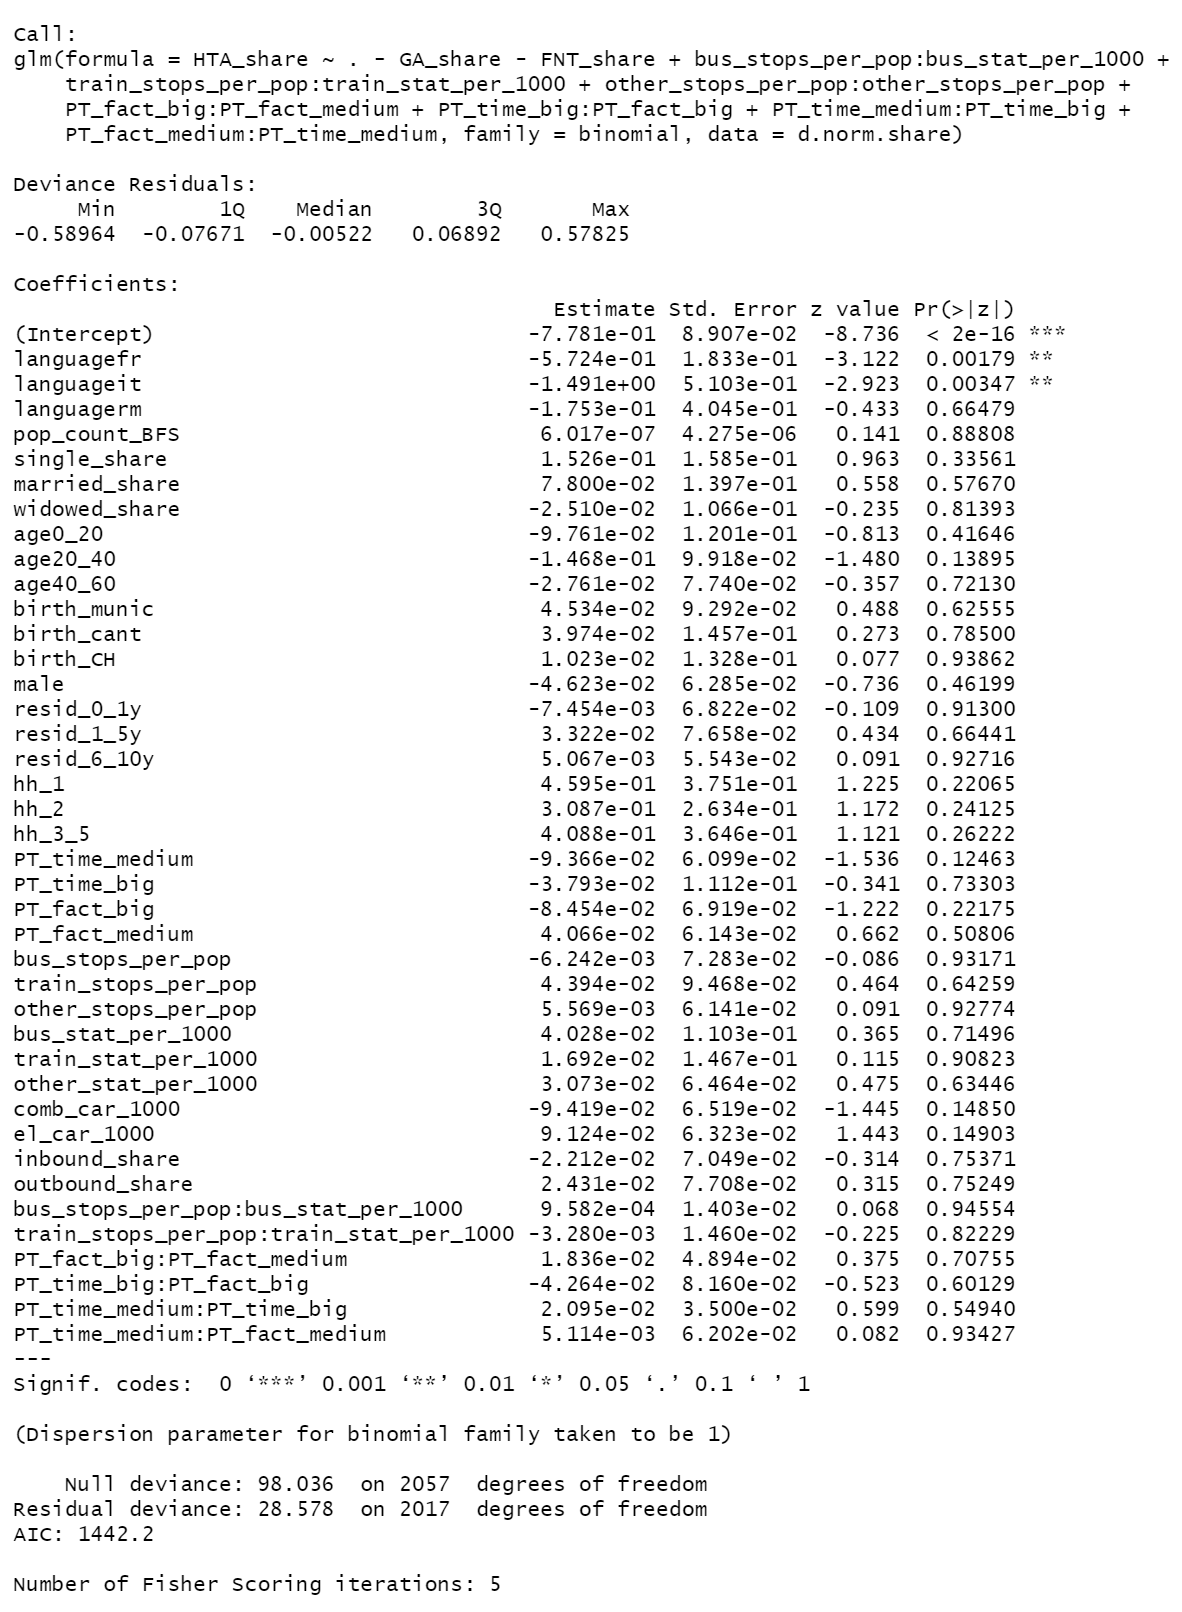
\includegraphics{GLM_HTA_share_01.png}

\begin{Shaded}
\begin{Highlighting}[]
\DocumentationTok{\#\#\#\#\#\#\#\#\#\#\#\#\#\#\# Stepwise parameter selection forward and backwards!\#\#\#\#\#\#\#\#\#\#\#}
\NormalTok{glm.HTA.share}\FloatTok{.02} \OtherTok{\textless{}{-}} \FunctionTok{stepAIC}\NormalTok{(glm.HTA.share}\FloatTok{.01}\NormalTok{, }\AttributeTok{direction=}\StringTok{"both"}\NormalTok{, }\AttributeTok{trace=}\ConstantTok{FALSE}\NormalTok{)}
\FunctionTok{summary}\NormalTok{(glm.HTA.share}\FloatTok{.02}\NormalTok{)}
\end{Highlighting}
\end{Shaded}

\begin{verbatim}
## 
## Call:
## glm(formula = HTA_share ~ language + age20_40 + PT_fact_big + 
##     comb_car_1000 + el_car_1000, family = binomial, data = d.norm.share)
## 
## Deviance Residuals: 
##      Min        1Q    Median        3Q       Max  
## -0.57252  -0.09774  -0.00596   0.08716   0.59063  
## 
## Coefficients:
##               Estimate Std. Error z value Pr(>|z|)    
## (Intercept)   -0.75976    0.06050 -12.559  < 2e-16 ***
## languagefr    -0.57742    0.12413  -4.652 3.29e-06 ***
## languageit    -1.33328    0.29795  -4.475 7.65e-06 ***
## languagerm    -0.09659    0.33562  -0.288   0.7735    
## age20_40      -0.09506    0.05286  -1.799   0.0721 .  
## PT_fact_big   -0.10075    0.05687  -1.772   0.0764 .  
## comb_car_1000 -0.11601    0.05681  -2.042   0.0411 *  
## el_car_1000    0.10418    0.05345   1.949   0.0513 .  
## ---
## Signif. codes:  0 '***' 0.001 '**' 0.01 '*' 0.05 '.' 0.1 ' ' 1
## 
## (Dispersion parameter for binomial family taken to be 1)
## 
##     Null deviance: 98.036  on 2057  degrees of freedom
## Residual deviance: 40.345  on 2050  degrees of freedom
## AIC: 1380
## 
## Number of Fisher Scoring iterations: 5
\end{verbatim}

Here, the stepwise parameter selection looks a bit better, giving still
5 significant parameters (including language with three manifestations)
instead of 3 as it is the case for the GA. In order to achieve a
consistent procedure, a linear model is nevertheless made again in order
to transfer the variables relevant there into the next run of the GLM.

\hypertarget{linear-model-lm-hta}{%
\subsubsection{Linear Model (LM) (HTA)}\label{linear-model-lm-hta}}

Now the linear model will be identified:

\begin{Shaded}
\begin{Highlighting}[]
\CommentTok{\# Model with all predictors including defined interaction terms}
\NormalTok{lm.count.HTA }\OtherTok{\textless{}{-}} \FunctionTok{lm}\NormalTok{(HTA\_BFS }\SpecialCharTok{\textasciitilde{}}\NormalTok{ . }\SpecialCharTok{{-}}\NormalTok{GA\_BFS }\SpecialCharTok{{-}}\NormalTok{ fn\_tck\_BFS }
                    \SpecialCharTok{+}\NormalTok{ bus\_count}\SpecialCharTok{:}\NormalTok{bus\_stat}
                    \SpecialCharTok{+}\NormalTok{ train\_count}\SpecialCharTok{:}\NormalTok{train\_stat}
                    \SpecialCharTok{+}\NormalTok{ other\_count}\SpecialCharTok{:}\NormalTok{other\_stat}
                    \SpecialCharTok{+}\NormalTok{ PT\_fact\_big}\SpecialCharTok{:}\NormalTok{PT\_fact\_medium}
                    \SpecialCharTok{+}\NormalTok{ PT\_time\_big}\SpecialCharTok{:}\NormalTok{PT\_fact\_big}
                    \SpecialCharTok{+}\NormalTok{ PT\_time\_medium}\SpecialCharTok{:}\NormalTok{PT\_time\_big}
                    \SpecialCharTok{+}\NormalTok{ PT\_fact\_medium}\SpecialCharTok{:}\NormalTok{PT\_time\_medium,}
                  \AttributeTok{data =}\NormalTok{ d.norm.count.train) }


\DocumentationTok{\#\#\# Stepwise selection of parameters:}
\NormalTok{lm.count.HTA2 }\OtherTok{\textless{}{-}}\NormalTok{ MASS}\SpecialCharTok{::}\FunctionTok{stepAIC}\NormalTok{(lm.count.HTA, }\AttributeTok{direction =} \StringTok{"both"}\NormalTok{, }\AttributeTok{trace =} \ConstantTok{FALSE}\NormalTok{)}
\FunctionTok{summary}\NormalTok{(lm.count.HTA2)}
\end{Highlighting}
\end{Shaded}

\begin{verbatim}
## 
## Call:
## lm(formula = HTA_BFS ~ single_count_BFS + married_count_BFS + 
##     widowed_count_BFS + age0_20cnt + age20_40cnt + age40_60cnt + 
##     birth_munic_cnt + birth_cant_cnt + male_cnt + resid_1_5y_cnt + 
##     hh_1_cnt + hh_2_cnt + hh_3_5_cnt + PT_time_medium + PT_time_big + 
##     bus_count + other_count + bus_stat + train_stat + Combustion + 
##     Electric + language + PT_fact_big + PT_fact_medium + PT_fact_big:PT_fact_medium + 
##     PT_time_big:PT_fact_big + PT_time_medium:PT_time_big, data = d.norm.count.train)
## 
## Residuals:
##      Min       1Q   Median       3Q      Max 
## -1.31512 -0.12024  0.01251  0.13003  1.11071 
## 
## Coefficients:
##                             Estimate Std. Error t value Pr(>|t|)    
## (Intercept)                 1.909632   0.569091   3.356  0.00081 ***
## single_count_BFS            0.959184   0.094025  10.201  < 2e-16 ***
## married_count_BFS           0.501435   0.088806   5.646 1.93e-08 ***
## widowed_count_BFS          -0.067731   0.030561  -2.216  0.02681 *  
## age0_20cnt                 -0.329199   0.056057  -5.873 5.20e-09 ***
## age20_40cnt                -0.562584   0.061035  -9.217  < 2e-16 ***
## age40_60cnt                -0.132514   0.085851  -1.544  0.12290    
## birth_munic_cnt             0.010673   0.006452   1.654  0.09827 .  
## birth_cant_cnt              0.036827   0.011494   3.204  0.00138 ** 
## male_cnt                   -0.376998   0.147149  -2.562  0.01050 *  
## resid_1_5y_cnt              0.058926   0.030368   1.940  0.05250 .  
## hh_1_cnt                    0.104446   0.037930   2.754  0.00596 ** 
## hh_2_cnt                    0.566852   0.056548  10.024  < 2e-16 ***
## hh_3_5_cnt                  0.529794   0.086027   6.158 9.25e-10 ***
## PT_time_medium             -0.278742   0.105355  -2.646  0.00823 ** 
## PT_time_big                 0.035386   0.116022   0.305  0.76041    
## bus_count                  -0.011167   0.003470  -3.219  0.00131 ** 
## other_count                 0.017394   0.002112   8.237 3.61e-16 ***
## bus_stat                    0.034386   0.013360   2.574  0.01015 *  
## train_stat                  0.042100   0.012841   3.278  0.00107 ** 
## Combustion                 -0.453069   0.043979 -10.302  < 2e-16 ***
## Electric                    0.129083   0.016090   8.023 1.97e-15 ***
## languagefr                 -0.400267   0.017720 -22.588  < 2e-16 ***
## languageit                 -1.035626   0.038597 -26.832  < 2e-16 ***
## languagerm                 -0.067453   0.038989  -1.730  0.08381 .  
## PT_fact_big                 0.364195   0.205748   1.770  0.07690 .  
## PT_fact_medium             -0.125112   0.076773  -1.630  0.10338    
## PT_fact_big:PT_fact_medium  0.138148   0.045125   3.061  0.00224 ** 
## PT_time_big:PT_fact_big    -0.184802   0.044445  -4.158 3.38e-05 ***
## PT_time_medium:PT_time_big  0.039938   0.024178   1.652  0.09877 .  
## ---
## Signif. codes:  0 '***' 0.001 '**' 0.01 '*' 0.05 '.' 0.1 ' ' 1
## 
## Residual standard error: 0.2116 on 1618 degrees of freedom
## Multiple R-squared:  0.975,  Adjusted R-squared:  0.9746 
## F-statistic:  2178 on 29 and 1618 DF,  p-value: < 2.2e-16
\end{verbatim}

The stepAIC function gives me now a suggested formula, what can be used
for a further try of the GLM. The coefficients show the weights.

\hypertarget{adapted-glm-with-family-quasibinomial-hta}{%
\subsubsection{\texorpdfstring{Adapted GLM with family quasibinomial
(HTA)\newline}{Adapted GLM with family quasibinomial (HTA)}}\label{adapted-glm-with-family-quasibinomial-hta}}

Also here, all parameters present after the stepwise parameter deletion
with the function `stepAIC' for the linear model, will be included in
the next GLM model:

Let's have a look at the next model run:

\begin{Shaded}
\begin{Highlighting}[]
\CommentTok{\# New run of quasibinomial model}

\NormalTok{glm.HTA.share}\FloatTok{.03} \OtherTok{\textless{}{-}} \FunctionTok{glm}\NormalTok{(HTA\_share }\SpecialCharTok{\textasciitilde{}}\NormalTok{ single\_share }\SpecialCharTok{+}\NormalTok{ married\_share }\SpecialCharTok{+}\NormalTok{ widowed\_share }\SpecialCharTok{+} 
\NormalTok{      age0\_20 }\SpecialCharTok{+}\NormalTok{ age20\_40 }\SpecialCharTok{+}\NormalTok{ age40\_60 }\SpecialCharTok{+}\NormalTok{ birth\_munic }\SpecialCharTok{+}\NormalTok{ birth\_cant }\SpecialCharTok{+}\NormalTok{ male }\SpecialCharTok{+}\NormalTok{ resid\_1\_5y }\SpecialCharTok{+} 
\NormalTok{      hh\_1 }\SpecialCharTok{+}\NormalTok{ hh\_2 }\SpecialCharTok{+}\NormalTok{ hh\_3\_5 }\SpecialCharTok{+}\NormalTok{ PT\_time\_medium }\SpecialCharTok{+}\NormalTok{ PT\_time\_big }\SpecialCharTok{+}\NormalTok{ bus\_stops\_per\_pop }\SpecialCharTok{+} 
\NormalTok{      other\_stops\_per\_pop }\SpecialCharTok{+}\NormalTok{ bus\_stat\_per\_1000 }\SpecialCharTok{+}\NormalTok{ train\_stat\_per\_1000 }\SpecialCharTok{+}\NormalTok{ comb\_car\_1000 }\SpecialCharTok{+}
\NormalTok{      el\_car\_1000 }\SpecialCharTok{+}\NormalTok{ language }\SpecialCharTok{+}\NormalTok{ PT\_fact\_big }\SpecialCharTok{+}\NormalTok{ PT\_fact\_medium }\SpecialCharTok{+}\NormalTok{ PT\_fact\_big}\SpecialCharTok{:}\NormalTok{PT\_fact\_medium }\SpecialCharTok{+} 
\NormalTok{      PT\_time\_big}\SpecialCharTok{:}\NormalTok{PT\_fact\_big }\SpecialCharTok{+}\NormalTok{ PT\_time\_medium}\SpecialCharTok{:}\NormalTok{PT\_time\_big, }
      \AttributeTok{family =}\NormalTok{ quasibinomial, }\AttributeTok{data=}\NormalTok{d.norm.share)}

\FunctionTok{summary}\NormalTok{(glm.HTA.share}\FloatTok{.03}\NormalTok{)}
\end{Highlighting}
\end{Shaded}

\begin{verbatim}
## 
## Call:
## glm(formula = HTA_share ~ single_share + married_share + widowed_share + 
##     age0_20 + age20_40 + age40_60 + birth_munic + birth_cant + 
##     male + resid_1_5y + hh_1 + hh_2 + hh_3_5 + PT_time_medium + 
##     PT_time_big + bus_stops_per_pop + other_stops_per_pop + bus_stat_per_1000 + 
##     train_stat_per_1000 + comb_car_1000 + el_car_1000 + language + 
##     PT_fact_big + PT_fact_medium + PT_fact_big:PT_fact_medium + 
##     PT_time_big:PT_fact_big + PT_time_medium:PT_time_big, family = quasibinomial, 
##     data = d.norm.share)
## 
## Deviance Residuals: 
##      Min        1Q    Median        3Q       Max  
## -0.60783  -0.07742  -0.00520   0.06695   0.58016  
## 
## Coefficients:
##                             Estimate Std. Error t value Pr(>|t|)    
## (Intercept)                -0.777410   0.009976 -77.930  < 2e-16 ***
## single_share                0.155443   0.018526   8.391  < 2e-16 ***
## married_share               0.077070   0.016495   4.672 3.17e-06 ***
## widowed_share              -0.030970   0.012505  -2.477 0.013346 *  
## age0_20                    -0.101718   0.014152  -7.188 9.23e-13 ***
## age20_40                   -0.157035   0.011403 -13.771  < 2e-16 ***
## age40_60                   -0.026701   0.009225  -2.894 0.003840 ** 
## birth_munic                 0.035909   0.008016   4.480 7.89e-06 ***
## birth_cant                  0.030798   0.007590   4.058 5.15e-05 ***
## male                       -0.048081   0.007469  -6.438 1.51e-10 ***
## resid_1_5y                  0.028209   0.008668   3.255 0.001155 ** 
## hh_1                        0.460956   0.044837  10.281  < 2e-16 ***
## hh_2                        0.315471   0.030755  10.257  < 2e-16 ***
## hh_3_5                      0.412828   0.043206   9.555  < 2e-16 ***
## PT_time_medium             -0.093181   0.007222 -12.902  < 2e-16 ***
## PT_time_big                -0.033584   0.012043  -2.789 0.005340 ** 
## bus_stops_per_pop          -0.011185   0.008502  -1.315 0.188494    
## other_stops_per_pop         0.027215   0.005865   4.641 3.70e-06 ***
## bus_stat_per_1000           0.044728   0.010572   4.231 2.43e-05 ***
## train_stat_per_1000         0.026425   0.006343   4.166 3.23e-05 ***
## comb_car_1000              -0.096891   0.007569 -12.800  < 2e-16 ***
## el_car_1000                 0.087232   0.007389  11.805  < 2e-16 ***
## languagefr                 -0.565877   0.020978 -26.974  < 2e-16 ***
## languageit                 -1.513014   0.058383 -25.915  < 2e-16 ***
## languagerm                 -0.179718   0.048199  -3.729 0.000198 ***
## PT_fact_big                -0.088425   0.008117 -10.894  < 2e-16 ***
## PT_fact_medium              0.037766   0.007212   5.237 1.80e-07 ***
## PT_fact_big:PT_fact_medium  0.018738   0.005709   3.282 0.001047 ** 
## PT_time_big:PT_fact_big    -0.044536   0.009448  -4.714 2.60e-06 ***
## PT_time_medium:PT_time_big  0.020038   0.004117   4.867 1.22e-06 ***
## ---
## Signif. codes:  0 '***' 0.001 '**' 0.01 '*' 0.05 '.' 0.1 ' ' 1
## 
## (Dispersion parameter for quasibinomial family taken to be 0.01448846)
## 
##     Null deviance: 98.036  on 2057  degrees of freedom
## Residual deviance: 29.329  on 2028  degrees of freedom
## AIC: NA
## 
## Number of Fisher Scoring iterations: 5
\end{verbatim}

still, 30 parameters are too much here. IN order to reduce further, the
6 lowest t values are removed. =\textgreater{} here to get all
parameters with high t value, marked as *** The coefficient t-value is a
measure of how many standard deviations our coefficient estimate is far
away from 0

\begin{Shaded}
\begin{Highlighting}[]
\NormalTok{glm.HTA.share}\FloatTok{.04} \OtherTok{\textless{}{-}} \FunctionTok{glm}\NormalTok{(HTA\_share }\SpecialCharTok{\textasciitilde{}}\NormalTok{ single\_share }\SpecialCharTok{+}\NormalTok{ married\_share }\SpecialCharTok{+}\NormalTok{ age0\_20 }\SpecialCharTok{+} 
\NormalTok{                      age20\_40 }\SpecialCharTok{+}\NormalTok{ birth\_munic }\SpecialCharTok{+}\NormalTok{ birth\_cant }\SpecialCharTok{+}\NormalTok{ male }\SpecialCharTok{+}\NormalTok{ hh\_1 }\SpecialCharTok{+}\NormalTok{ hh\_2 }\SpecialCharTok{+} 
\NormalTok{                      hh\_3\_5 }\SpecialCharTok{+}\NormalTok{ PT\_time\_medium }\SpecialCharTok{+}\NormalTok{ other\_stops\_per\_pop }\SpecialCharTok{+} 
\NormalTok{                      bus\_stat\_per\_1000 }\SpecialCharTok{+}\NormalTok{ train\_stat\_per\_1000 }\SpecialCharTok{+}\NormalTok{ comb\_car\_1000 }\SpecialCharTok{+} 
\NormalTok{                      el\_car\_1000 }\SpecialCharTok{+}\NormalTok{ language }\SpecialCharTok{+}\NormalTok{ PT\_fact\_big }\SpecialCharTok{+}\NormalTok{ PT\_fact\_medium }\SpecialCharTok{+} 
\NormalTok{                      PT\_time\_big}\SpecialCharTok{:}\NormalTok{PT\_fact\_big }\SpecialCharTok{+}\NormalTok{ PT\_time\_medium}\SpecialCharTok{:}\NormalTok{PT\_time\_big,}
                \AttributeTok{family =}\NormalTok{ quasibinomial, }\AttributeTok{data=}\NormalTok{d.norm.share)}

\FunctionTok{summary}\NormalTok{(glm.HTA.share}\FloatTok{.04}\NormalTok{)}
\end{Highlighting}
\end{Shaded}

\begin{verbatim}
## 
## Call:
## glm(formula = HTA_share ~ single_share + married_share + age0_20 + 
##     age20_40 + birth_munic + birth_cant + male + hh_1 + hh_2 + 
##     hh_3_5 + PT_time_medium + other_stops_per_pop + bus_stat_per_1000 + 
##     train_stat_per_1000 + comb_car_1000 + el_car_1000 + language + 
##     PT_fact_big + PT_fact_medium + PT_time_big:PT_fact_big + 
##     PT_time_medium:PT_time_big, family = quasibinomial, data = d.norm.share)
## 
## Deviance Residuals: 
##      Min        1Q    Median        3Q       Max  
## -0.63082  -0.07697  -0.00346   0.06843   0.64535  
## 
## Coefficients:
##                             Estimate Std. Error t value Pr(>|t|)    
## (Intercept)                -0.768876   0.008840 -86.981  < 2e-16 ***
## single_share                0.161107   0.016373   9.840  < 2e-16 ***
## married_share               0.082751   0.014655   5.647 1.86e-08 ***
## age0_20                    -0.078824   0.013112  -6.011 2.17e-09 ***
## age20_40                   -0.127007   0.009235 -13.753  < 2e-16 ***
## birth_munic                 0.019953   0.007184   2.777 0.005532 ** 
## birth_cant                  0.024491   0.007235   3.385 0.000725 ***
## male                       -0.048770   0.007141  -6.829 1.12e-11 ***
## hh_1                        0.464048   0.044626  10.399  < 2e-16 ***
## hh_2                        0.327810   0.030394  10.785  < 2e-16 ***
## hh_3_5                      0.408575   0.042244   9.672  < 2e-16 ***
## PT_time_medium             -0.099748   0.007189 -13.875  < 2e-16 ***
## other_stops_per_pop         0.024943   0.005830   4.279 1.97e-05 ***
## bus_stat_per_1000           0.033598   0.008752   3.839 0.000127 ***
## train_stat_per_1000         0.025985   0.006207   4.186 2.96e-05 ***
## comb_car_1000              -0.105916   0.007430 -14.255  < 2e-16 ***
## el_car_1000                 0.099659   0.007164  13.911  < 2e-16 ***
## languagefr                 -0.544974   0.019877 -27.417  < 2e-16 ***
## languageit                 -1.592514   0.049827 -31.961  < 2e-16 ***
## languagerm                 -0.227308   0.043953  -5.172 2.55e-07 ***
## PT_fact_big                -0.090835   0.008148 -11.148  < 2e-16 ***
## PT_fact_medium              0.044095   0.007122   6.192 7.19e-10 ***
## PT_fact_big:PT_time_big    -0.043322   0.009482  -4.569 5.20e-06 ***
## PT_time_medium:PT_time_big  0.019171   0.003992   4.802 1.68e-06 ***
## ---
## Signif. codes:  0 '***' 0.001 '**' 0.01 '*' 0.05 '.' 0.1 ' ' 1
## 
## (Dispersion parameter for quasibinomial family taken to be 0.01483236)
## 
##     Null deviance: 98.036  on 2057  degrees of freedom
## Residual deviance: 30.050  on 2034  degrees of freedom
## AIC: NA
## 
## Number of Fisher Scoring iterations: 5
\end{verbatim}

At least, all parameters left appear to be highly significant here. The
model evaluation in a later section will show how this model performs.

\hypertarget{modelling-fare-network-tickets-fnt}{%
\subsection{Modelling Fare Network Tickets
(FNT)}\label{modelling-fare-network-tickets-fnt}}

The same procedure shown for the GA and HTA is also valid for the FNT
and will not be commented the same way here.

\hypertarget{generalized-linear-model-glm-with-family-binomial-fnt}{%
\subsubsection{Generalized Linear Model (GLM) with family ``Binomial''
(FNT)}\label{generalized-linear-model-glm-with-family-binomial-fnt}}

The same procedure as used for the GA is applied here for the FNT. The
first step with the selection of interactions is not done here, as the
analysis from the GA should be enough for all target variables. The
earlier defined interaction terms are taken as well into this model
here:

The first run is done by using all possible influence factors and the
already defined interaction terms:

\begin{Shaded}
\begin{Highlighting}[]
\DocumentationTok{\#\#\#\#\#  Modelling GLM for FNT with share data:}

\DocumentationTok{\#\# Interactions: For interaction terms, the same selection is taken as described}
\DocumentationTok{\#\# for the GA model above:}

\DocumentationTok{\#\#\#\#\#\#\#\#\#\#\#\#\#\#\#\#\#\#\# Model set up 01 \#\#\#\#\#\#\#\#\#\#\#\#\#\#\#\#\#\#\#\#\#\#}
\NormalTok{glm.FNT.share}\FloatTok{.01} \OtherTok{\textless{}{-}} \FunctionTok{glm}\NormalTok{(FNT\_share }\SpecialCharTok{\textasciitilde{}}\NormalTok{ . }\SpecialCharTok{{-}}\NormalTok{ GA\_share }\SpecialCharTok{{-}}\NormalTok{ HTA\_share}
                    \SpecialCharTok{+}\NormalTok{ bus\_stops\_per\_pop}\SpecialCharTok{:}\NormalTok{bus\_stat\_per\_1000}
                    \SpecialCharTok{+}\NormalTok{ train\_stops\_per\_pop}\SpecialCharTok{:}\NormalTok{train\_stat\_per\_1000}
                    \SpecialCharTok{+}\NormalTok{ other\_stops\_per\_pop}\SpecialCharTok{:}\NormalTok{other\_stops\_per\_pop}
                    \SpecialCharTok{+}\NormalTok{ PT\_fact\_big}\SpecialCharTok{:}\NormalTok{PT\_fact\_medium}
                    \SpecialCharTok{+}\NormalTok{ PT\_time\_big}\SpecialCharTok{:}\NormalTok{PT\_fact\_big}
                    \SpecialCharTok{+}\NormalTok{ PT\_time\_medium}\SpecialCharTok{:}\NormalTok{PT\_time\_big}
                    \SpecialCharTok{+}\NormalTok{ PT\_fact\_medium}\SpecialCharTok{:}\NormalTok{PT\_time\_medium, }
                \AttributeTok{family =}\NormalTok{ binomial, }\AttributeTok{data=}\NormalTok{d.norm.share)}
\FunctionTok{summary}\NormalTok{(glm.FNT.share}\FloatTok{.01}\NormalTok{)}
\end{Highlighting}
\end{Shaded}

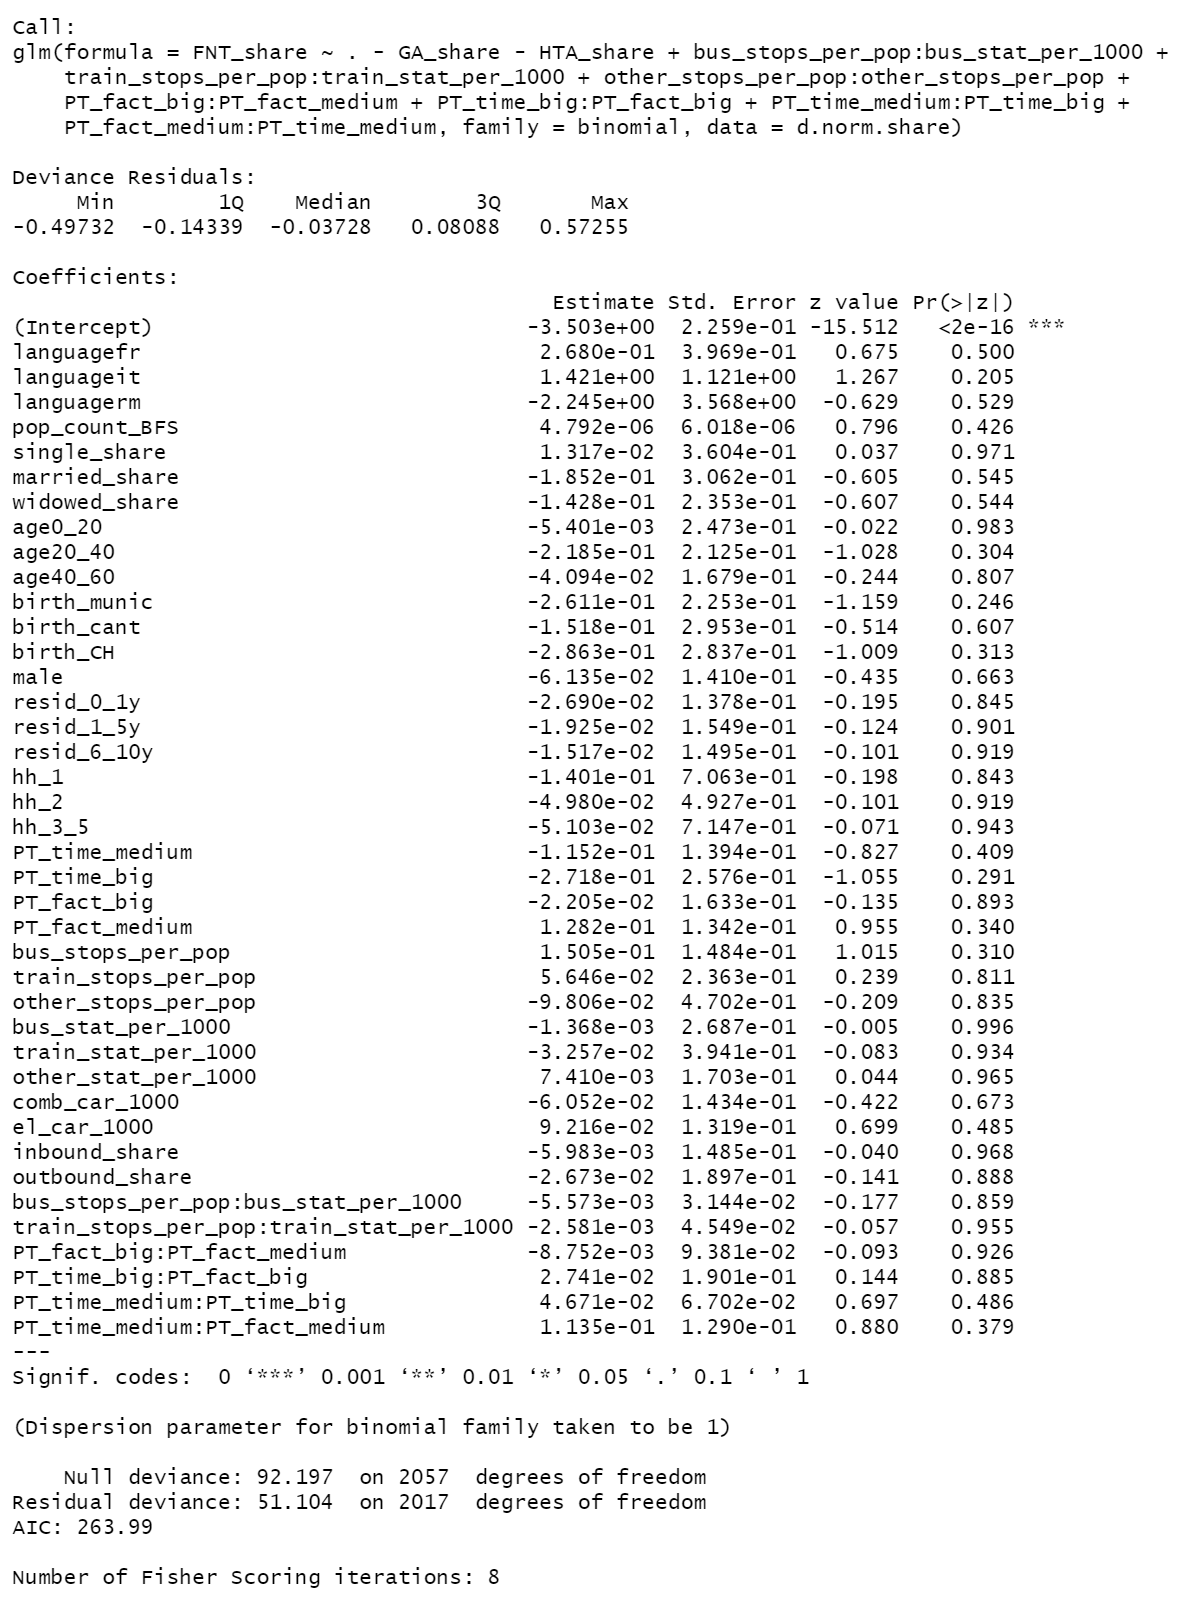
\includegraphics{GLM_FNT_share_01.png}

\begin{Shaded}
\begin{Highlighting}[]
\DocumentationTok{\#\#\#\#\#\#\#\#\#\#\#\#\#\#\# Stepwise parameter selection forward and backwards!\#\#\#\#\#\#\#\#\#\#\#}
\NormalTok{glm.FNT.share}\FloatTok{.02} \OtherTok{\textless{}{-}} \FunctionTok{stepAIC}\NormalTok{(glm.FNT.share}\FloatTok{.01}\NormalTok{, }\AttributeTok{direction=}\StringTok{"both"}\NormalTok{, }\AttributeTok{trace=}\ConstantTok{FALSE}\NormalTok{)}
\FunctionTok{summary}\NormalTok{(glm.FNT.share}\FloatTok{.02}\NormalTok{)}
\end{Highlighting}
\end{Shaded}

\begin{verbatim}
## 
## Call:
## glm(formula = FNT_share ~ married_share + age20_40 + birth_munic + 
##     birth_cant + birth_CH + hh_3_5, family = binomial, data = d.norm.share)
## 
## Deviance Residuals: 
##      Min        1Q    Median        3Q       Max  
## -0.45127  -0.16718  -0.04545   0.09600   0.61640  
## 
## Coefficients:
##               Estimate Std. Error z value Pr(>|z|)    
## (Intercept)    -3.2556     0.1229 -26.494  < 2e-16 ***
## married_share  -0.2654     0.1243  -2.134  0.03282 *  
## age20_40       -0.2474     0.1231  -2.010  0.04447 *  
## birth_munic    -0.3640     0.1579  -2.304  0.02121 *  
## birth_cant     -0.3967     0.1713  -2.316  0.02055 *  
## birth_CH       -0.5639     0.1820  -3.099  0.00194 ** 
## hh_3_5          0.1900     0.1015   1.872  0.06116 .  
## ---
## Signif. codes:  0 '***' 0.001 '**' 0.01 '*' 0.05 '.' 0.1 ' ' 1
## 
## (Dispersion parameter for binomial family taken to be 1)
## 
##     Null deviance: 92.197  on 2057  degrees of freedom
## Residual deviance: 63.130  on 2051  degrees of freedom
## AIC: 195.38
## 
## Number of Fisher Scoring iterations: 6
\end{verbatim}

Here, the stepwise parameter selection gives back 6 significant
parameters. In order to achieve a consistent procedure, a linear model
is nevertheless made again in order to transfer the variables relevant
there into the next run of the GLM.

\hypertarget{linear-model-lm-fnt}{%
\subsubsection{Linear Model (LM) (FNT)}\label{linear-model-lm-fnt}}

Now the linear model will be identified:

\begin{Shaded}
\begin{Highlighting}[]
\CommentTok{\# Model with all predictors including defined interaction terms}
\NormalTok{lm.count.FNT }\OtherTok{\textless{}{-}} \FunctionTok{lm}\NormalTok{(fn\_tck\_BFS }\SpecialCharTok{\textasciitilde{}}\NormalTok{ . }\SpecialCharTok{{-}}\NormalTok{GA\_BFS }\SpecialCharTok{{-}}\NormalTok{ HTA\_BFS }
                    \SpecialCharTok{+}\NormalTok{ bus\_count}\SpecialCharTok{:}\NormalTok{bus\_stat}
                    \SpecialCharTok{+}\NormalTok{ train\_count}\SpecialCharTok{:}\NormalTok{train\_stat}
                    \SpecialCharTok{+}\NormalTok{ other\_count}\SpecialCharTok{:}\NormalTok{other\_stat}
                    \SpecialCharTok{+}\NormalTok{ PT\_fact\_big}\SpecialCharTok{:}\NormalTok{PT\_fact\_medium}
                    \SpecialCharTok{+}\NormalTok{ PT\_time\_big}\SpecialCharTok{:}\NormalTok{PT\_fact\_big}
                    \SpecialCharTok{+}\NormalTok{ PT\_time\_medium}\SpecialCharTok{:}\NormalTok{PT\_time\_big}
                    \SpecialCharTok{+}\NormalTok{ PT\_fact\_medium}\SpecialCharTok{:}\NormalTok{PT\_time\_medium, }
                  \AttributeTok{data =}\NormalTok{ d.norm.count.train) }

\NormalTok{lm.count.FNT2 }\OtherTok{\textless{}{-}}\NormalTok{ MASS}\SpecialCharTok{::}\FunctionTok{stepAIC}\NormalTok{(lm.count.FNT, }\AttributeTok{direction =} \StringTok{"both"}\NormalTok{, }\AttributeTok{trace =} \ConstantTok{FALSE}\NormalTok{)}
\FunctionTok{summary}\NormalTok{(lm.count.FNT2)}
\end{Highlighting}
\end{Shaded}

\begin{verbatim}
## 
## Call:
## lm(formula = fn_tck_BFS ~ single_count_BFS + married_count_BFS + 
##     age20_40cnt + age40_60cnt + birth_munic_cnt + birth_cant_cnt + 
##     birth_CH_cnt + male_cnt + resid_1_5y_cnt + hh_1_cnt + PT_time_medium + 
##     PT_time_big + bus_count + other_count + train_count + bus_stat + 
##     other_stat + train_stat + Combustion + Electric + language + 
##     PT_fact_big + PT_fact_medium + bus_count:bus_stat + train_count:train_stat + 
##     other_count:other_stat + PT_time_big:PT_fact_big + PT_time_medium:PT_time_big + 
##     PT_time_medium:PT_fact_medium, data = d.norm.count.train)
## 
## Residuals:
##     Min      1Q  Median      3Q     Max 
## -4.6400 -0.6441  0.1699  0.8092  2.6282 
## 
## Coefficients:
##                                Estimate Std. Error t value Pr(>|t|)    
## (Intercept)                   19.679425   3.114060   6.320 3.38e-10 ***
## single_count_BFS               2.516410   0.437647   5.750 1.07e-08 ***
## married_count_BFS             -1.630979   0.433251  -3.765 0.000173 ***
## age20_40cnt                   -1.612113   0.293202  -5.498 4.45e-08 ***
## age40_60cnt                   -0.820709   0.408271  -2.010 0.044575 *  
## birth_munic_cnt               -0.246423   0.035751  -6.893 7.82e-12 ***
## birth_cant_cnt                 0.230309   0.082383   2.796 0.005242 ** 
## birth_CH_cnt                  -0.192380   0.079059  -2.433 0.015066 *  
## male_cnt                       1.658677   0.752646   2.204 0.027679 *  
## resid_1_5y_cnt                 0.396994   0.161273   2.462 0.013935 *  
## hh_1_cnt                      -0.219162   0.137817  -1.590 0.111975    
## PT_time_medium                -4.237189   0.670591  -6.319 3.41e-10 ***
## PT_time_big                   -4.423755   0.636492  -6.950 5.27e-12 ***
## bus_count                      0.015476   0.019059   0.812 0.416891    
## other_count                   -0.021848   0.028539  -0.766 0.444051    
## train_count                    0.005934   0.016333   0.363 0.716433    
## bus_stat                      -0.505571   0.205689  -2.458 0.014078 *  
## other_stat                     0.766786   0.449621   1.705 0.088311 .  
## train_stat                    -0.946986   0.613927  -1.543 0.123146    
## Combustion                     0.465439   0.240100   1.939 0.052734 .  
## Electric                       0.387637   0.085822   4.517 6.74e-06 ***
## languagefr                    -0.046085   0.089294  -0.516 0.605855    
## languageit                     1.561043   0.215131   7.256 6.15e-13 ***
## languagerm                    -1.495839   0.212774  -7.030 3.03e-12 ***
## PT_fact_big                   -3.266925   1.081583  -3.021 0.002563 ** 
## PT_fact_medium                -1.926268   0.906598  -2.125 0.033761 *  
## bus_count:bus_stat             0.037508   0.014299   2.623 0.008796 ** 
## train_count:train_stat         0.097347   0.047771   2.038 0.041733 *  
## other_count:other_stat        -0.079439   0.046391  -1.712 0.087019 .  
## PT_time_big:PT_fact_big        0.677385   0.250065   2.709 0.006823 ** 
## PT_time_medium:PT_time_big     0.709501   0.129642   5.473 5.13e-08 ***
## PT_time_medium:PT_fact_medium  0.570787   0.219871   2.596 0.009517 ** 
## ---
## Signif. codes:  0 '***' 0.001 '**' 0.01 '*' 0.05 '.' 0.1 ' ' 1
## 
## Residual standard error: 1.155 on 1616 degrees of freedom
## Multiple R-squared:  0.6438, Adjusted R-squared:  0.637 
## F-statistic: 94.23 on 31 and 1616 DF,  p-value: < 2.2e-16
\end{verbatim}

The stepAIC function gives us now a suggested formula, what can be used
for a further try of the GLM. The coefficients show the weights of the
parameters.

\hypertarget{adapted-glm-with-family-quasibinomial-fnt}{%
\subsubsection{Adapted GLM with family quasibinomial
(FNT)}\label{adapted-glm-with-family-quasibinomial-fnt}}

Also here, all parameters present after the stepwise parameter deletion
with the function `stepAIC' for the linear model, will be included in
the next GLM model:

\begin{Shaded}
\begin{Highlighting}[]
\CommentTok{\# New run of quasibinomial model}

\NormalTok{glm.FNT.share}\FloatTok{.03} \OtherTok{\textless{}{-}} \FunctionTok{glm}\NormalTok{(FNT\_share }\SpecialCharTok{\textasciitilde{}}\NormalTok{ single\_share }\SpecialCharTok{+}\NormalTok{ married\_share }\SpecialCharTok{+} 
\NormalTok{                          age20\_40 }\SpecialCharTok{+}\NormalTok{ age40\_60 }\SpecialCharTok{+}\NormalTok{ birth\_munic }\SpecialCharTok{+}\NormalTok{ birth\_cant }\SpecialCharTok{+} 
\NormalTok{                          birth\_CH }\SpecialCharTok{+}\NormalTok{ male }\SpecialCharTok{+}\NormalTok{ resid\_1\_5y }\SpecialCharTok{+}\NormalTok{ hh\_1 }\SpecialCharTok{+}\NormalTok{ PT\_time\_medium }\SpecialCharTok{+} 
\NormalTok{                          PT\_time\_big }\SpecialCharTok{+}\NormalTok{ bus\_stops\_per\_pop }\SpecialCharTok{+}\NormalTok{ other\_stops\_per\_pop }\SpecialCharTok{+} 
\NormalTok{                          train\_stops\_per\_pop }\SpecialCharTok{+}\NormalTok{ bus\_stat\_per\_1000 }\SpecialCharTok{+} 
\NormalTok{                          other\_stat\_per\_1000 }\SpecialCharTok{+}\NormalTok{ train\_stat\_per\_1000 }\SpecialCharTok{+} 
\NormalTok{                          comb\_car\_1000 }\SpecialCharTok{+}\NormalTok{ el\_car\_1000 }\SpecialCharTok{+}\NormalTok{ language }\SpecialCharTok{+}\NormalTok{ PT\_fact\_big }\SpecialCharTok{+} 
\NormalTok{                          PT\_fact\_medium }\SpecialCharTok{+}\NormalTok{ bus\_stops\_per\_pop}\SpecialCharTok{:}\NormalTok{bus\_stat\_per\_1000 }\SpecialCharTok{+} 
\NormalTok{                          train\_stops\_per\_pop}\SpecialCharTok{:}\NormalTok{train\_stat\_per\_1000 }\SpecialCharTok{+} 
\NormalTok{                          other\_stops\_per\_pop}\SpecialCharTok{:}\NormalTok{other\_stat\_per\_1000 }\SpecialCharTok{+} 
\NormalTok{                          PT\_time\_big}\SpecialCharTok{:}\NormalTok{PT\_fact\_big }\SpecialCharTok{+}\NormalTok{ PT\_time\_medium}\SpecialCharTok{:}\NormalTok{PT\_time\_big }\SpecialCharTok{+} 
\NormalTok{                          PT\_time\_medium}\SpecialCharTok{:}\NormalTok{PT\_fact\_medium, }
                \AttributeTok{family =}\NormalTok{ quasibinomial, }\AttributeTok{data=}\NormalTok{d.norm.share)}

\FunctionTok{summary}\NormalTok{(glm.FNT.share}\FloatTok{.03}\NormalTok{)}
\end{Highlighting}
\end{Shaded}

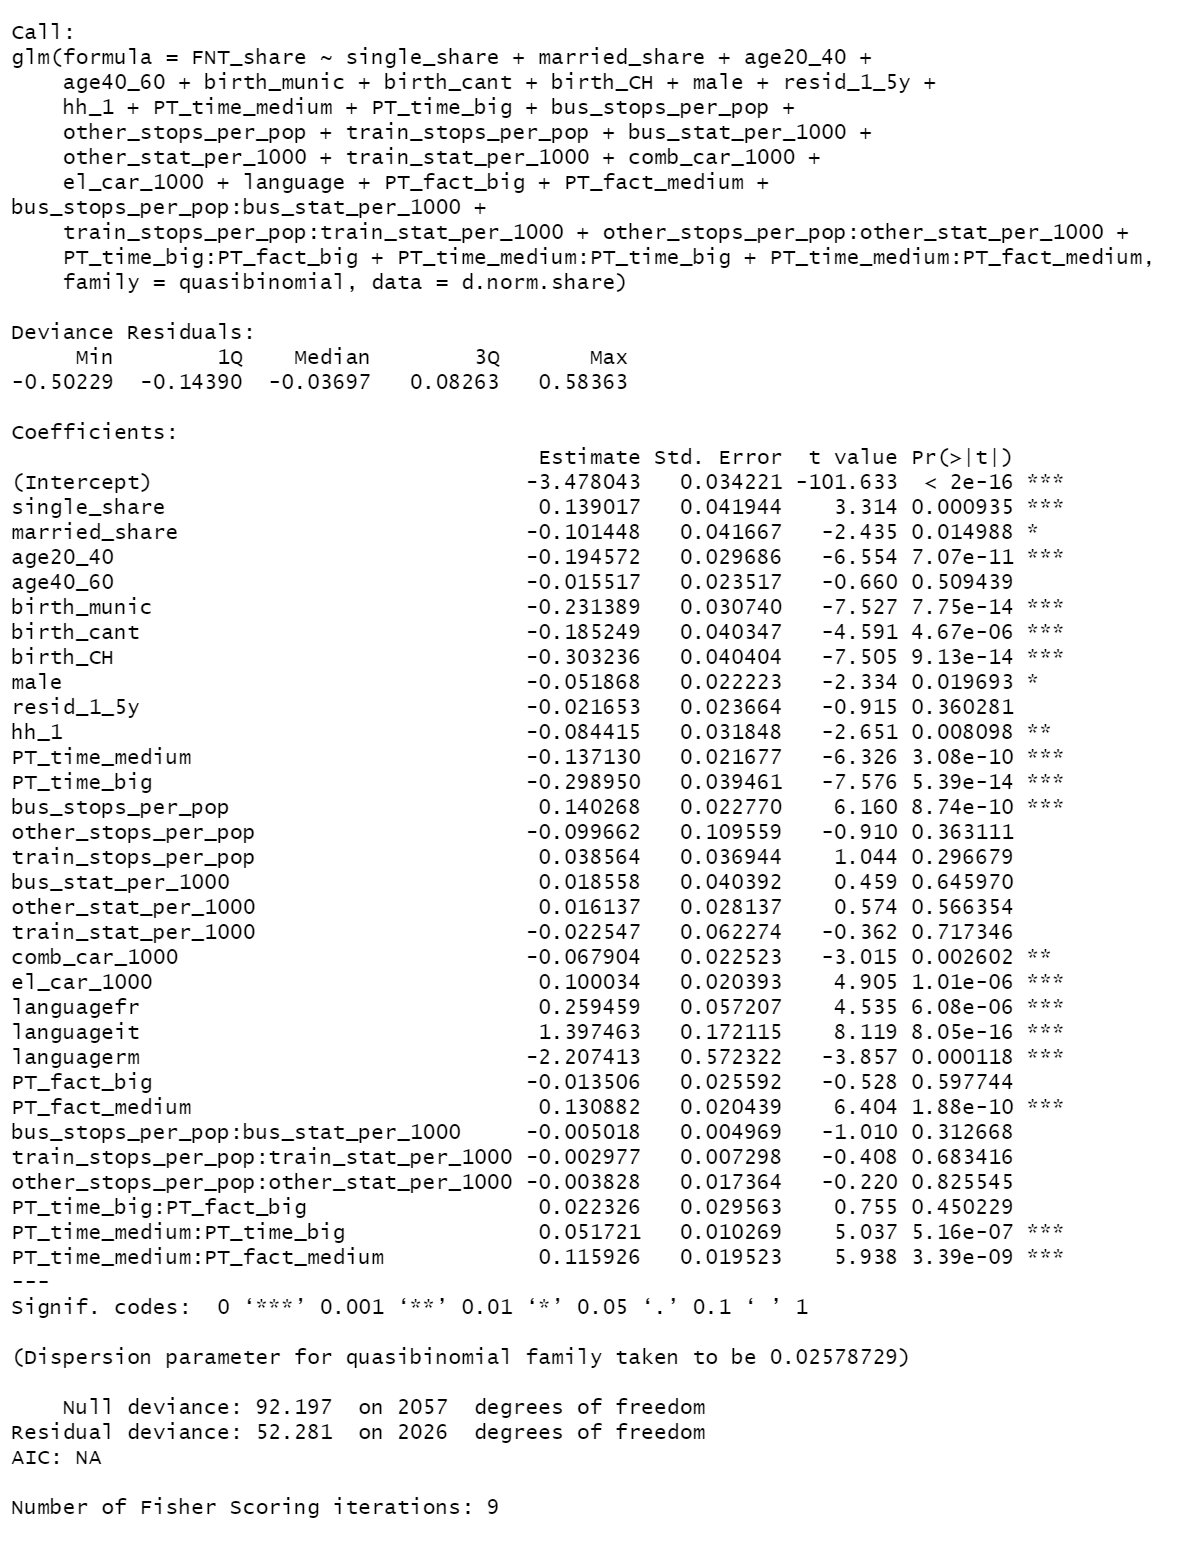
\includegraphics{GLM_FNT_share_03.png}

Still, 32 parameters are too much here. In order to reduce further,
about 10 - 15 parameters with the lowest t values should be removed. The
coefficient t-value is a measure of how many standard deviations our
coefficient estimate is far away from 0. This will be used as the
criterion to eliminate parameters from the model.

Now the final model with only selected parameters:

\begin{Shaded}
\begin{Highlighting}[]
\NormalTok{glm.FNT.share}\FloatTok{.04} \OtherTok{\textless{}{-}} \FunctionTok{glm}\NormalTok{(FNT\_share }\SpecialCharTok{\textasciitilde{}}\NormalTok{ single\_share }\SpecialCharTok{+}\NormalTok{ married\_share }\SpecialCharTok{+} 
\NormalTok{                          age20\_40 }\SpecialCharTok{+}\NormalTok{ birth\_munic }\SpecialCharTok{+}\NormalTok{ birth\_cant }\SpecialCharTok{+} 
\NormalTok{                          birth\_CH }\SpecialCharTok{+}\NormalTok{ male }\SpecialCharTok{+}\NormalTok{ hh\_1 }\SpecialCharTok{+}\NormalTok{ PT\_time\_medium }\SpecialCharTok{+} 
\NormalTok{                          PT\_time\_big }\SpecialCharTok{+}\NormalTok{ bus\_stops\_per\_pop }\SpecialCharTok{+} 
\NormalTok{                          comb\_car\_1000 }\SpecialCharTok{+}\NormalTok{ el\_car\_1000 }\SpecialCharTok{+}\NormalTok{ language }\SpecialCharTok{+} 
\NormalTok{                          PT\_fact\_medium }\SpecialCharTok{+}\NormalTok{ PT\_time\_medium}\SpecialCharTok{:}\NormalTok{PT\_time\_big }\SpecialCharTok{+} 
\NormalTok{                          PT\_time\_medium}\SpecialCharTok{:}\NormalTok{PT\_fact\_medium, }
                \AttributeTok{family =}\NormalTok{ quasibinomial, }\AttributeTok{data=}\NormalTok{d.norm.share)}

\FunctionTok{summary}\NormalTok{(glm.FNT.share}\FloatTok{.04}\NormalTok{)}
\end{Highlighting}
\end{Shaded}

\begin{verbatim}
## 
## Call:
## glm(formula = FNT_share ~ single_share + married_share + age20_40 + 
##     birth_munic + birth_cant + birth_CH + male + hh_1 + PT_time_medium + 
##     PT_time_big + bus_stops_per_pop + comb_car_1000 + el_car_1000 + 
##     language + PT_fact_medium + PT_time_medium:PT_time_big + 
##     PT_time_medium:PT_fact_medium, family = quasibinomial, data = d.norm.share)
## 
## Deviance Residuals: 
##      Min        1Q    Median        3Q       Max  
## -0.50178  -0.14437  -0.03755   0.08272   0.58142  
## 
## Coefficients:
##                                Estimate Std. Error  t value Pr(>|t|)    
## (Intercept)                   -3.484747   0.032447 -107.399  < 2e-16 ***
## single_share                   0.130257   0.041502    3.139 0.001722 ** 
## married_share                 -0.103897   0.041123   -2.527 0.011595 *  
## age20_40                      -0.189211   0.025547   -7.406 1.89e-13 ***
## birth_munic                   -0.214817   0.027843   -7.715 1.87e-14 ***
## birth_cant                    -0.168764   0.036214   -4.660 3.36e-06 ***
## birth_CH                      -0.291671   0.038001   -7.675 2.54e-14 ***
## male                          -0.053364   0.019979   -2.671 0.007623 ** 
## hh_1                          -0.080547   0.030481   -2.643 0.008292 ** 
## PT_time_medium                -0.139599   0.021375   -6.531 8.22e-11 ***
## PT_time_big                   -0.303469   0.037653   -8.060 1.29e-15 ***
## bus_stops_per_pop              0.130462   0.017896    7.290 4.42e-13 ***
## comb_car_1000                 -0.071031   0.022331   -3.181 0.001491 ** 
## el_car_1000                    0.095915   0.020276    4.730 2.39e-06 ***
## languagefr                     0.260900   0.054959    4.747 2.21e-06 ***
## languageit                     1.381175   0.138398    9.980  < 2e-16 ***
## languagerm                    -2.187709   0.570398   -3.835 0.000129 ***
## PT_fact_medium                 0.121513   0.018626    6.524 8.61e-11 ***
## PT_time_medium:PT_time_big     0.053436   0.009791    5.458 5.41e-08 ***
## PT_time_medium:PT_fact_medium  0.118022   0.019074    6.188 7.36e-10 ***
## ---
## Signif. codes:  0 '***' 0.001 '**' 0.01 '*' 0.05 '.' 0.1 ' ' 1
## 
## (Dispersion parameter for quasibinomial family taken to be 0.02576204)
## 
##     Null deviance: 92.197  on 2057  degrees of freedom
## Residual deviance: 52.523  on 2038  degrees of freedom
## AIC: NA
## 
## Number of Fisher Scoring iterations: 8
\end{verbatim}

At least, all parameters left appear to be highly significant here. The
model evaluation in a later section will show, how this model performs.
\newpage

\hypertarget{model-evaluation}{%
\section{MODEL EVALUATION}\label{model-evaluation}}

This section assesses the model quality of the different models
developed. The chapter is divided into a statistical part, which deals
with key figures, and a graphical part, where the model quality can be
assessed visually.

\hypertarget{model-fitness}{%
\subsection{Model fitness}\label{model-fitness}}

In this part, the statistical measuring of the RMSE and the Rsquare
value is central. To do this, the following formula is formulated:

\hypertarget{function-for-model-evaluation}{%
\subsubsection{Function for Model
Evaluation}\label{function-for-model-evaluation}}

For the evaluation of our models we will use the following function,
which displays the RMSE and the R\_squared for our predicted values.

Linear models and Generalized linear models with family binomial have
slightly different properties in the measurement of model quality. For
the linear models the adjusted R-squared value can be calculated
additionally, for the GLM the explained variance can be calculated by
the residual deviation and the null deviation.

\begin{Shaded}
\begin{Highlighting}[]
\NormalTok{eval\_results }\OtherTok{\textless{}{-}} \ControlFlowTok{function}\NormalTok{(true, predicted) \{}
\NormalTok{  SSE }\OtherTok{\textless{}{-}} \FunctionTok{sum}\NormalTok{((predicted }\SpecialCharTok{{-}}\NormalTok{ true)}\SpecialCharTok{\^{}}\DecValTok{2}\NormalTok{, }\AttributeTok{na.rm =} \ConstantTok{TRUE}\NormalTok{)}
\NormalTok{  SST }\OtherTok{\textless{}{-}} \FunctionTok{sum}\NormalTok{((true }\SpecialCharTok{{-}} \FunctionTok{mean}\NormalTok{(true, }\AttributeTok{na.rm =} \ConstantTok{TRUE}\NormalTok{))}\SpecialCharTok{\^{}}\DecValTok{2}\NormalTok{, }\AttributeTok{na.rm =} \ConstantTok{TRUE}\NormalTok{)}
\NormalTok{  R\_square }\OtherTok{\textless{}{-}} \DecValTok{1} \SpecialCharTok{{-}}\NormalTok{ SSE }\SpecialCharTok{/}\NormalTok{ SST}
\NormalTok{  RMSE }\OtherTok{=} \FunctionTok{sqrt}\NormalTok{(SSE}\SpecialCharTok{/}\FunctionTok{length}\NormalTok{(true))}

\CommentTok{\# Model performance metrics}
  \FunctionTok{data.frame}\NormalTok{(}\AttributeTok{RMSE =}\NormalTok{ RMSE,}
           \AttributeTok{Rsquare =}\NormalTok{ R\_square)}
\NormalTok{\}}

\CommentTok{\# Adjusted R square for linear model}
\NormalTok{adj\_r2 }\OtherTok{\textless{}{-}} \ControlFlowTok{function}\NormalTok{(lm\_model) \{}
  \FunctionTok{summary}\NormalTok{(lm\_model)}\SpecialCharTok{$}\NormalTok{adj.r.squared}
\NormalTok{\}}

\CommentTok{\# deviance explained by glm:}
\NormalTok{dev\_exp\_glm }\OtherTok{\textless{}{-}} \ControlFlowTok{function}\NormalTok{(glm\_model) \{}
  \FunctionTok{with}\NormalTok{(}\FunctionTok{summary}\NormalTok{(glm\_model), }\DecValTok{1} \SpecialCharTok{{-}}\NormalTok{ deviance}\SpecialCharTok{/}\NormalTok{null.deviance)}
\NormalTok{\}}
\end{Highlighting}
\end{Shaded}

\hypertarget{model-fitness-of-lm-and-glm-models}{%
\subsubsection{Model fitness of LM and GLM
models:}\label{model-fitness-of-lm-and-glm-models}}

The various measurements such as RMSE and Rsquare are now summarised in
a table for all models. The table is defined as follows:

\begin{Shaded}
\begin{Highlighting}[]
\NormalTok{model\_evaluation }\OtherTok{\textless{}{-}} \FunctionTok{data.frame}\NormalTok{(}\StringTok{"Train\_RMSE"}\OtherTok{=}\DecValTok{0}\NormalTok{, }\StringTok{"Train\_R\^{}2"}\OtherTok{=}\DecValTok{0}\NormalTok{, }
           \StringTok{"Test\_RMSE"}\OtherTok{=}\DecValTok{0}\NormalTok{, }\StringTok{"Test\_R\^{}2"}\OtherTok{=}\DecValTok{0}\NormalTok{, }\StringTok{"nr\_param"}\OtherTok{=}\DecValTok{0}\NormalTok{, }\StringTok{"Dev.Expl\_Adj.R2"}\OtherTok{=}\DecValTok{0}\NormalTok{)}
\end{Highlighting}
\end{Shaded}

The RMSE and Rsquare value is measured both for the Train and Test
dataset individually, while the last field in the dataframe,
``nr\_param'', describes the complexity of the model with the number of
different parameters present.

The table is filled as the following, here with the example of the first
GLM model for the GA data:

\begin{Shaded}
\begin{Highlighting}[]
\DocumentationTok{\#\# Evaluating GLM 01 (original glm with all data) }
\NormalTok{model\_evaluation[}\StringTok{"GA\_GLM\_01"}\NormalTok{,] }\OtherTok{\textless{}{-}} \FunctionTok{c}\NormalTok{(}\FunctionTok{eval\_results}\NormalTok{(d.norm.share.train}\SpecialCharTok{$}\NormalTok{GA\_share,}
                                    \FunctionTok{predict}\NormalTok{(glm.share}\FloatTok{.01}\NormalTok{, d.norm.share.train, }
                                            \AttributeTok{type=}\StringTok{"response"}\NormalTok{)),}
                                 \FunctionTok{eval\_results}\NormalTok{(d.norm.share.test}\SpecialCharTok{$}\NormalTok{GA\_share, }
                                    \FunctionTok{predict}\NormalTok{(glm.share}\FloatTok{.01}\NormalTok{, d.norm.share.test, }
                                            \AttributeTok{type=}\StringTok{"response"}\NormalTok{)),}
\NormalTok{                                 glm.share}\FloatTok{.01}\SpecialCharTok{$}\NormalTok{rank,}
                                 \FunctionTok{dev\_exp\_glm}\NormalTok{(glm.share}\FloatTok{.01}\NormalTok{))}
\end{Highlighting}
\end{Shaded}

The original data is compared with the prediction each for the test and
Train dataset, using the above defined formula. With the
``rank''-option, the number of parameters are filled in the last step.
The same procedure is valid for all the other models including the ones
for the HTA and FNT data. It is not showed here in order to save some
space.

The filled table looks as the following:

\begin{Shaded}
\begin{Highlighting}[]
\FunctionTok{round}\NormalTok{(model\_evaluation, }\AttributeTok{digits=}\DecValTok{2}\NormalTok{) }
\end{Highlighting}
\end{Shaded}

\begin{verbatim}
##               Train_RMSE Train_R.2 Test_RMSE Test_R.2 nr_param Dev.Expl_Adj.R2
## GA_GLM_01           0.01      0.82      0.01     0.80      593            0.80
## GA_GLM_03           0.02      0.26      0.02     0.29        4            0.27
## GA_GLM_04           0.02      0.51      0.02     0.52       33            0.51
## GA_GLM_05           0.02      0.49      0.02     0.51       23            0.50
## GA_LM_01_log        0.44      0.90      0.44     0.90       40            0.90
## GA_LM_01_cnt      234.89      0.88    268.03     0.97       40            0.90
## GA_LM_02_log        0.44      0.90      0.44     0.90       33            0.90
## GA_LM_02_cnt      234.08      0.88    179.46     0.99       33            0.90
## HTA_GLM_01          0.05      0.71      0.05     0.72       41            0.71
## HTA_GLM_02          0.06      0.59      0.06     0.56        8            0.59
## HTA_GLM_03          0.05      0.70      0.05     0.71       30            0.70
## HTA_GLM_04          0.05      0.69      0.05     0.71       24            0.69
## HTA_LM_01_log       0.21      0.98      0.23     0.97       40            0.97
## HTA_LM_01_cnt     548.67      0.97    868.23     0.99       40            0.97
## HTA_LM_02_log       0.21      0.98      0.23     0.97       30            0.97
## HTA_LM_02_cnt     564.35      0.97   1245.56     0.98       30            0.97
## FNT_GLM_01          0.03      0.49      0.03     0.46       41            0.45
## FNT_GLM_02          0.03      0.38      0.04     0.30        7            0.32
## FNT_GLM_03          0.03      0.48      0.03     0.41       32            0.43
## FNT_GLM_04          0.03      0.48      0.03     0.41       20            0.43
## FNT_LM_01_log       1.14      0.64      1.17     0.66       40            0.64
## FNT_LM_01_cnt    1404.51     -0.44   2354.18     0.70       40            0.64
## FNT_LM_02_log       1.14      0.64      1.17     0.66       32            0.64
## FNT_LM_02_cnt    1379.88     -0.39   2352.50     0.70       32            0.64
\end{verbatim}

Basically, it can be seen that the linear models have a higher accuracy,
measured by the R-squared value. This is not surprising, however, since
in the count data the population size plays a role in most variables
even after normalization, both in the explanatory and target variables.
The more inhabitants a municipality has, the higher the number of
tickets sold on average, as well as the number of people who are men,
under 20 years of age, live in a one-person household or are divorced,
for example. That is also the reason why in principle work was done with
the shares. Nevertheless, the linear models were important to get an
idea of the most important influencing factors through the step-by-step
parameter elimination procedure with stepAIC.

Within the GLM for general subscriptions (GA), it is noticeable that the
various models differ greatly in the number of parameters used. The
model with all possible variables and interactions has almost 600
parameters, while the model after stepwise selection ``GA\_GLM\_02'' has
only 4. The explained variance drops from 80\% to 27\% herewith. Even if
only 4 variables can still explain a part, the loss of accuracy is too
great. Hence the approach of reducing the original parameters with the
stepwise selection from the linear model. In the end, 23 parameters were
defined that had an R-squared value of exactly 50 \%. This model
``GA\_GLM\_05'' builds the final model for the GA.

For the half-fare season tickets, the GLM model generally performs
better with higher accuracies between 71\% (all parameters after
stepwise selection from the linear model) and 59\% (model after stepwise
selection within the GLM-binomial environment). Here one could say that
the simplest model with only 8 parameters is accepted because it can
still explain 59\% of the variance. Since the procedure should be the
same for all target variables, parameters were nevertheless added here
again to reach the final model ``HTA\_GLM\_04'' with 24 parameters and
an explained variance of 69\%.

The procedure works least well for the Fare Network Tickets. With the
same procedure, 43\% of the variance can finally be explained with a
model consisting of 20 parameters (``FNT\_GLM\_04''). Here it is also
noticeable that the linear model with an R-squared value of 0.64 is
clearly below the corresponding values for GA (0.90) and Half-Fare
Travelcards (HTA, 0.97).

\hypertarget{graphical-evaluation}{%
\subsection{Graphical evaluation}\label{graphical-evaluation}}

The second part of the evaluation is a graphical analysis of the
forecast values with the real values. This shows the characteristics of
the different models and in particular graphically shows how strong the
dispersion is compared to the true value.

\hypertarget{ga-models}{%
\subsubsection{GA models}\label{ga-models}}

To start, the graphical evaluation of all different GLM models of the
General Season Ticket (GA).

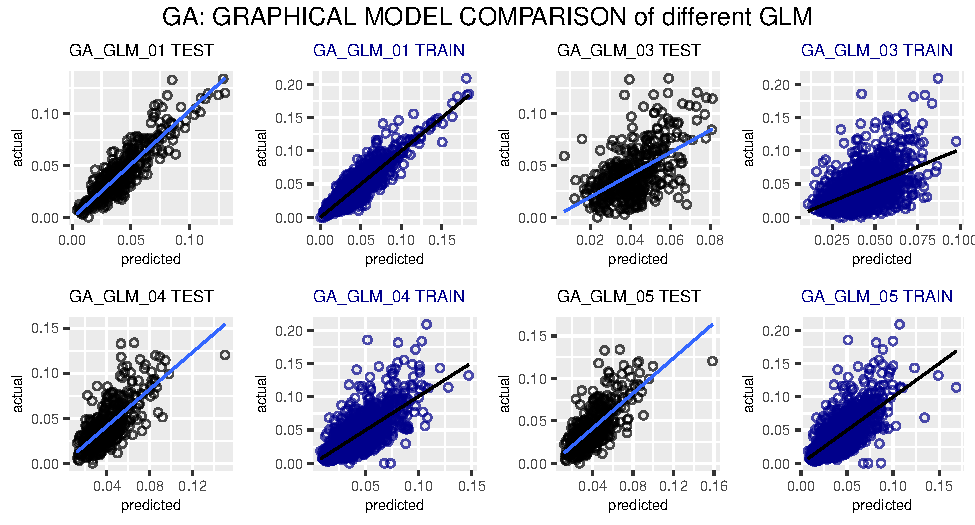
\includegraphics{Influence_factors_files/figure-latex/2.28_GA_model_eval_graphically-1.pdf}

\hypertarget{hta-models}{%
\subsubsection{HTA models}\label{hta-models}}

And now all graphical evaluations of the different GLM models of the
Half Fare Travelcards (HTA).

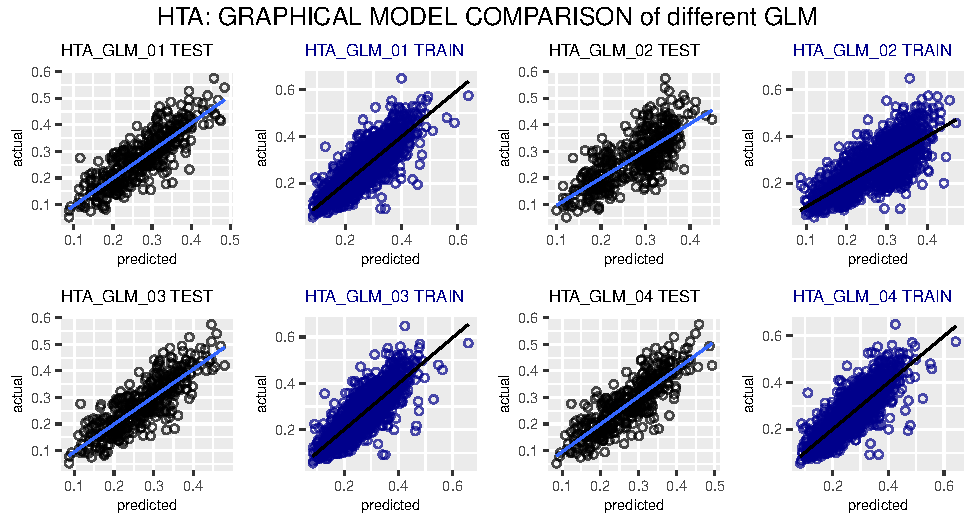
\includegraphics{Influence_factors_files/figure-latex/2.29_HTA_model_eval_graphically-1.pdf}

\hypertarget{fnt-models}{%
\subsubsection{FNT models}\label{fnt-models}}

Here the graphical evaluation of all different GLM models of the Fare
Network Tickets (FNT).

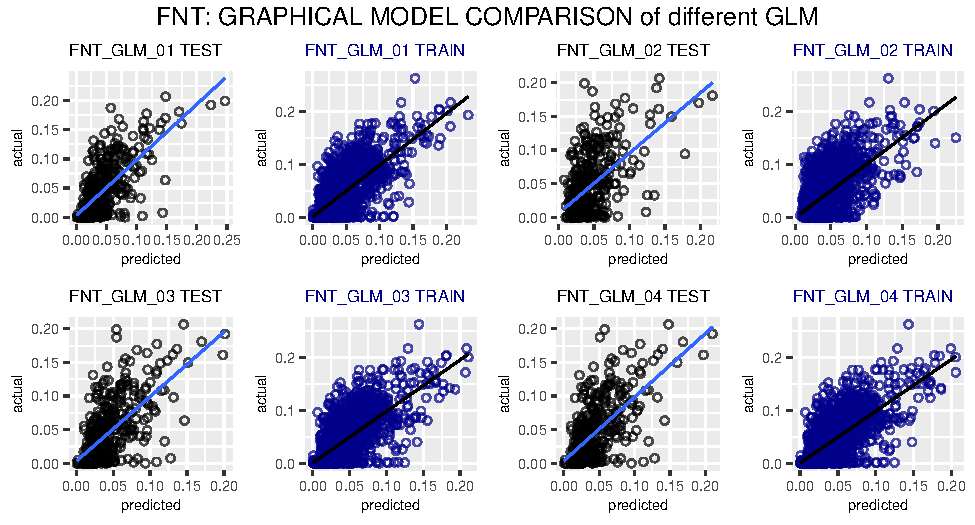
\includegraphics{Influence_factors_files/figure-latex/2.30_FNT_model_eval_graphically-1.pdf}

\hypertarget{comparing-estimates-of-the-different-models}{%
\subsection{Comparing estimates of the different
models}\label{comparing-estimates-of-the-different-models}}

Out of the graphical analysis, the final models can be confirmed as the
following:

\begin{itemize}
\tightlist
\item
  GA\_GLM\_05
\item
  HTA\_GLM\_04
\item
  FNT\_GLM\_04
\end{itemize}

From these models, all estimates can be compared and stored in a
separate table. As the all have normalized variables, the estimates can
be compared as the weight is the same for all herewith.

\begin{Shaded}
\begin{Highlighting}[]
\NormalTok{ga.coef }\OtherTok{\textless{}{-}} \FunctionTok{data.frame}\NormalTok{(}\FunctionTok{as.list}\NormalTok{(glm.share}\FloatTok{.05}\SpecialCharTok{$}\NormalTok{coefficients))}

\NormalTok{hta.coef }\OtherTok{\textless{}{-}} \FunctionTok{data.frame}\NormalTok{(}\FunctionTok{as.list}\NormalTok{(glm.HTA.share}\FloatTok{.04}\SpecialCharTok{$}\NormalTok{coefficients))}

\NormalTok{fnt.coef }\OtherTok{\textless{}{-}} \FunctionTok{data.frame}\NormalTok{(}\FunctionTok{as.list}\NormalTok{(glm.FNT.share}\FloatTok{.04}\SpecialCharTok{$}\NormalTok{coefficients))}

\NormalTok{inf\_factors }\OtherTok{\textless{}{-}} \FunctionTok{rbind.fill}\NormalTok{(ga.coef, hta.coef, fnt.coef)}
\NormalTok{inf\_factors }\OtherTok{\textless{}{-}} \FunctionTok{t}\NormalTok{(inf\_factors)}
\FunctionTok{colnames}\NormalTok{(inf\_factors) }\OtherTok{\textless{}{-}} \FunctionTok{c}\NormalTok{(}\StringTok{"GA\_share"}\NormalTok{, }\StringTok{"HTA\_share"}\NormalTok{, }\StringTok{"FNT\_share"}\NormalTok{)}

\DocumentationTok{\#\#\# Write csv}
\FunctionTok{write.csv}\NormalTok{(inf\_factors, }\AttributeTok{file=}\StringTok{"inf\_factors.csv"}\NormalTok{)}
\end{Highlighting}
\end{Shaded}

All estimates can be plottes against each other to recognize
similarities between GA, HTA and FNT:

\begin{Shaded}
\begin{Highlighting}[]
\NormalTok{lowerFn }\OtherTok{\textless{}{-}} \ControlFlowTok{function}\NormalTok{(data, mapping, }\AttributeTok{method =} \StringTok{"lm"}\NormalTok{, ...) \{}
\NormalTok{  p }\OtherTok{\textless{}{-}} \FunctionTok{ggplot}\NormalTok{(}\AttributeTok{data =}\NormalTok{ data, }\AttributeTok{mapping =}\NormalTok{ mapping) }\SpecialCharTok{+}
    \FunctionTok{geom\_point}\NormalTok{(}\AttributeTok{colour =} \StringTok{"blue"}\NormalTok{, }\AttributeTok{size=}\FloatTok{1.2}\NormalTok{) }\SpecialCharTok{+}
    \FunctionTok{geom\_smooth}\NormalTok{(}\AttributeTok{method =}\NormalTok{ method, }\AttributeTok{color =} \StringTok{"black"}\NormalTok{, ...)}
\NormalTok{  p}
\NormalTok{\}}


\FunctionTok{ggpairs}\NormalTok{(}\FunctionTok{data.frame}\NormalTok{(inf\_factors[}\DecValTok{2}\SpecialCharTok{:}\DecValTok{32}\NormalTok{,]),}
        \AttributeTok{lower =} \FunctionTok{list}\NormalTok{(}\AttributeTok{continuous=} \FunctionTok{wrap}\NormalTok{(lowerFn, }\AttributeTok{method =} \StringTok{"lm"}\NormalTok{)),}
        \AttributeTok{diag =} \FunctionTok{list}\NormalTok{(}\AttributeTok{continuous =} \FunctionTok{wrap}\NormalTok{(}\StringTok{"barDiag"}\NormalTok{, }\AttributeTok{colour =} \StringTok{"blue"}\NormalTok{)),}
        \AttributeTok{upper =} \FunctionTok{list}\NormalTok{(}\AttributeTok{continuous =} \FunctionTok{wrap}\NormalTok{(}\StringTok{"cor"}\NormalTok{, }\AttributeTok{size =} \DecValTok{6}\NormalTok{))) }\SpecialCharTok{+} 
  \FunctionTok{ggtitle}\NormalTok{(}\StringTok{"Comparison of MODEL ESTIMATES for the GA{-}, HTA{-} and FNT{-}model"}\NormalTok{)}
\end{Highlighting}
\end{Shaded}

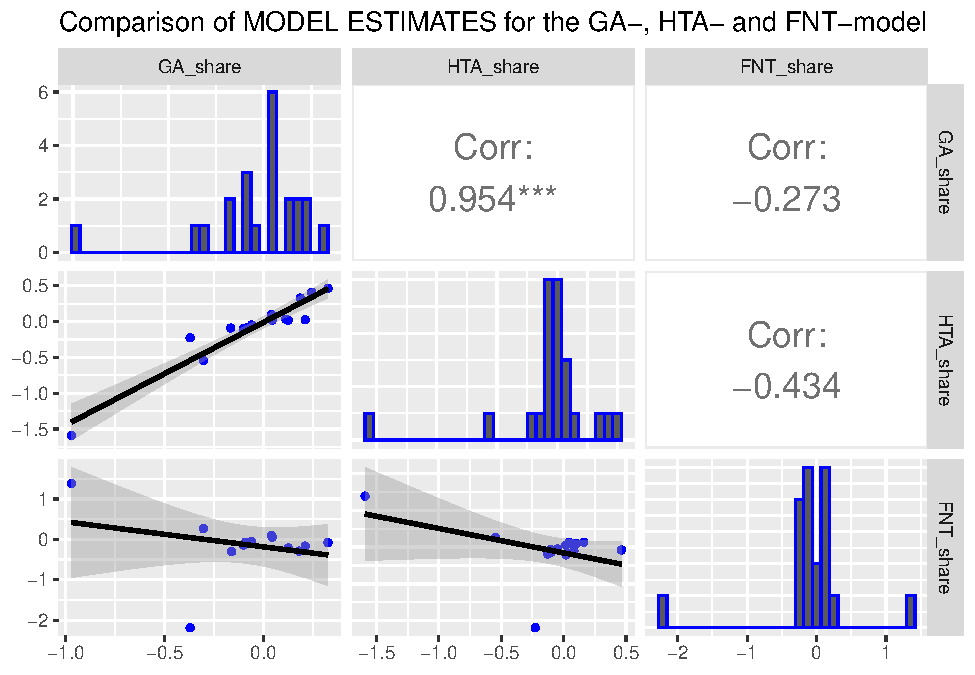
\includegraphics{Influence_factors_files/figure-latex/2.32_model_estimates_comparison-1.pdf}
The estimates for GA and HTA are strongly correlating with a correlation
value of 0.95! That means that the estimates for the both models are
very similar, so high values in one estimate for the GA are correlating
with high values in the same estimate for the HTA model. The FNT-model
is behaving completely different with negative correlation values
against the other two models. What, if we just look at the share values
directly and compare them?

\begin{Shaded}
\begin{Highlighting}[]
\FunctionTok{ggpairs}\NormalTok{(}\FunctionTok{data.frame}\NormalTok{(d.share[,}\FunctionTok{c}\NormalTok{(}\StringTok{"GA\_share"}\NormalTok{, }\StringTok{"HTA\_share"}\NormalTok{, }\StringTok{"FNT\_share"}\NormalTok{)]),}
        \AttributeTok{lower =} \FunctionTok{list}\NormalTok{(}\AttributeTok{continuous=} \FunctionTok{wrap}\NormalTok{(lowerFn, }\AttributeTok{method =} \StringTok{"lm"}\NormalTok{)),}
        \AttributeTok{diag =} \FunctionTok{list}\NormalTok{(}\AttributeTok{continuous =} \FunctionTok{wrap}\NormalTok{(}\StringTok{"barDiag"}\NormalTok{, }\AttributeTok{colour =} \StringTok{"blue"}\NormalTok{)),}
        \AttributeTok{upper =} \FunctionTok{list}\NormalTok{(}\AttributeTok{continuous =} \FunctionTok{wrap}\NormalTok{(}\StringTok{"cor"}\NormalTok{, }\AttributeTok{size =} \DecValTok{6}\NormalTok{))) }\SpecialCharTok{+} 
  \FunctionTok{ggtitle}\NormalTok{(}\StringTok{"Comparison of SHARE VALUES for GA, HTA and FNT"}\NormalTok{) }
\end{Highlighting}
\end{Shaded}

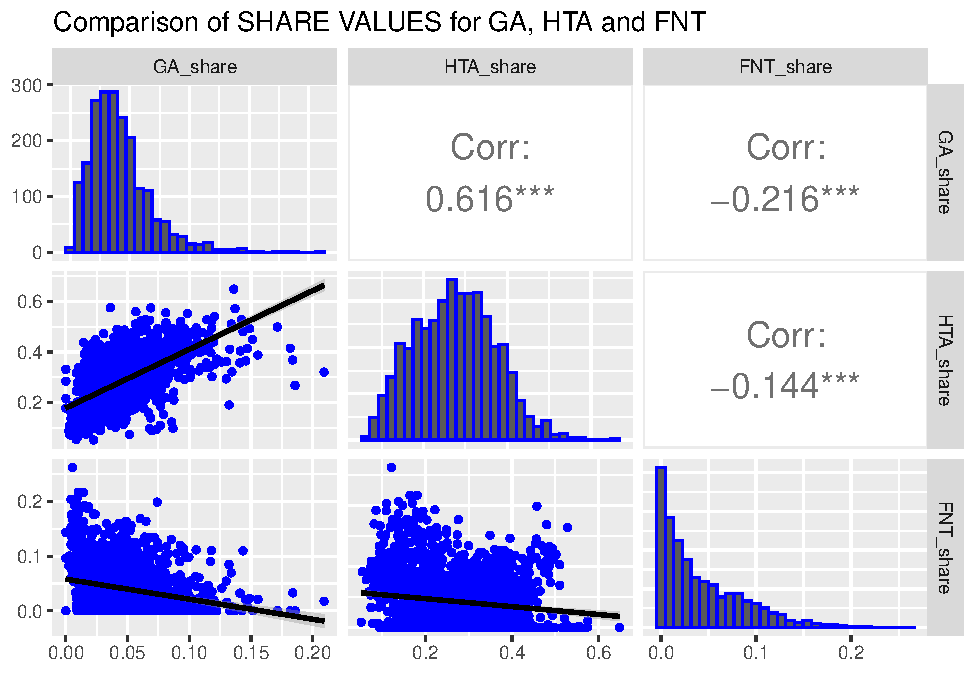
\includegraphics{Influence_factors_files/figure-latex/2.33_share_comparison-1.pdf}
Similar correlation values can be found here as well. It seems that the
proportions for GA and HTA behave very similarly. In municipalities with
a high proportion of GA travelcards, half-fare cards are often also
represented more frequently. On the other hand, it is the other way
round with regard to the fare network tickets. The greater the
proportion of GA or half-fare cards, the smaller the proportion of group
season tickets tends to be. \emph{literature ?}

\hypertarget{parameter-selection-for-cluster-analysis}{%
\subsection{Parameter selection for Cluster
Analysis}\label{parameter-selection-for-cluster-analysis}}

The different estimates values of the individual parameters are shown in
the Tableau Book ``Influence factors''.

All values in the table ``inf\_factors'' are taken into the cluster
analysis, which marks the next section of this script. For this purpose,
a separate file is created, which reduces the original dataset to the
relevant factors:

I build an extra dataframe with these variables, using the original
share dataset:

\begin{Shaded}
\begin{Highlighting}[]
\FunctionTok{rownames}\NormalTok{(inf\_factors)}
\end{Highlighting}
\end{Shaded}

\begin{verbatim}
##  [1] "X.Intercept."                  "age0_20"                      
##  [3] "birth_munic"                   "birth_cant"                   
##  [5] "birth_CH"                      "male"                         
##  [7] "resid_6_10y"                   "hh_1"                         
##  [9] "hh_2"                          "hh_3_5"                       
## [11] "PT_time_medium"                "PT_time_big"                  
## [13] "train_stops_per_pop"           "bus_stat_per_1000"            
## [15] "other_stat_per_1000"           "comb_car_1000"                
## [17] "el_car_1000"                   "languagefr"                   
## [19] "languageit"                    "languagerm"                   
## [21] "PT_fact_big"                   "PT_fact_big.PT_fact_medium"   
## [23] "PT_time_medium.PT_time_big"    "single_share"                 
## [25] "married_share"                 "age20_40"                     
## [27] "other_stops_per_pop"           "train_stat_per_1000"          
## [29] "PT_fact_medium"                "PT_fact_big.PT_time_big"      
## [31] "bus_stops_per_pop"             "PT_time_medium.PT_fact_medium"
\end{verbatim}

\begin{Shaded}
\begin{Highlighting}[]
\CommentTok{\# filtering out language (loading separate) and interaction terms}
\NormalTok{cl.an.input }\OtherTok{\textless{}{-}}\NormalTok{ d.norm.share[,}\FunctionTok{c}\NormalTok{(}\StringTok{"language"}\NormalTok{, }\FunctionTok{rownames}\NormalTok{(inf\_factors)}
\NormalTok{                               [}\FunctionTok{c}\NormalTok{(}\DecValTok{2}\SpecialCharTok{:}\DecValTok{17}\NormalTok{, }\DecValTok{21}\NormalTok{, }\DecValTok{24}\SpecialCharTok{:}\DecValTok{29}\NormalTok{, }\DecValTok{31}\NormalTok{)])]}
\end{Highlighting}
\end{Shaded}

\newpage

\hypertarget{cluster-analysis}{%
\section{CLUSTER ANALYSIS}\label{cluster-analysis}}

\emph{The best model of the different approaches will result in the
highest accuracy and a corresponding list of parameters which are
relevant and should be focussed on in the cluster analysis. Many,
diverse communities can make it difficult to find easily separable
clusters. Therefore, the first step of the cluster analysis is the
reduction of the data to the cantonal level. For this purpose, a
separate table must be created with a similar procedure as described in
chapter 5.2.2, with the shares calculated on this new level of
aggregation. Different options of cluster methods will be integrated in
the analysis. I will use an agglomerative clustering model to start,
which does not need a pre-defined number of clusters (Ward, 1963). This
is an advantage, especially because it is hard to estimate in advance
what number of groups will be useful at the end. Alternative models
would be a k-means clustering (partitioning method) with a given number
of clusters (MacQueen, 1967), a Generalized Mixture Model (GMM) which
uses statistical models and is not based simply on a distance measure
(Rasmussen, 1999), or even a density-based clustering like DBSCAN which
assigns points to clusters based on densities in the data, returning
also outliers (Ester et al., 1996).}

The primary aim of cluster analysis is to identify spatial distribution
patterns of certain characteristics with regard to relevant influencing
factors. This requires the integration of the shares that were also used
in the modelling. Particularly in cluster analysis, it is also important
to carry out a normalization so that all variables have the same
influence. Therefore, the normalized ``share'' table is used for the
cluster analysis.

\hypertarget{cluster-analysis-on-the-level-of-the-municipality}{%
\subsection{Cluster analysis on the level of the
municipality}\label{cluster-analysis-on-the-level-of-the-municipality}}

In a first attempt, the cluster analysis is carried out at the level of
the municipalities. Since this is an exploratory approach, primarily an
agglomerative procedure is used (Ward, 1963). With the reasonable number
of clusters obtained in this way, a k-means procedure is then applied
later, along with density-based DBSCAN clustering as a supplement.

\hypertarget{preparation-of-clustering}{%
\subsubsection{Preparation of
clustering}\label{preparation-of-clustering}}

As a basis for all clustering methods, a distance matrix must be
calculated. For a visual representation, the first two principal
components will then finally also have to be calculated so that as much
as possible of the variance present in the data can be represented
two-dimensionally.

\begin{Shaded}
\begin{Highlighting}[]
\CommentTok{\# Distance matrix}
\NormalTok{dp }\OtherTok{\textless{}{-}} \FunctionTok{dist}\NormalTok{(cl.an.input[,}\DecValTok{2}\SpecialCharTok{:}\DecValTok{25}\NormalTok{]) }\DocumentationTok{\#\# Euclidean distance}

\CommentTok{\# Principal components}
\NormalTok{PC.inf.fac }\OtherTok{\textless{}{-}} \FunctionTok{princomp}\NormalTok{(cl.an.input[,}\DecValTok{2}\SpecialCharTok{:}\DecValTok{25}\NormalTok{]) }\CommentTok{\# without language}
\FunctionTok{summary}\NormalTok{(PC.inf.fac, }\AttributeTok{loadings =} \ConstantTok{FALSE}\NormalTok{) }
\end{Highlighting}
\end{Shaded}

\begin{verbatim}
## Importance of components:
##                           Comp.1    Comp.2     Comp.3    Comp.4     Comp.5
## Standard deviation     2.0315533 1.7363261 1.48685577 1.3595490 1.28935785
## Proportion of Variance 0.1720506 0.1256789 0.09215895 0.0770530 0.06930216
## Cumulative Proportion  0.1720506 0.2977295 0.38988850 0.4669415 0.53624366
##                            Comp.6    Comp.7     Comp.8    Comp.9    Comp.10
## Standard deviation     1.23324400 1.1268066 1.02795786 1.0194851 0.97141932
## Proportion of Variance 0.06340126 0.0529296 0.04405046 0.0433273 0.03933809
## Cumulative Proportion  0.59964492 0.6525745 0.69662498 0.7399523 0.77929037
##                          Comp.11    Comp.12    Comp.13    Comp.14    Comp.15
## Standard deviation     0.8596227 0.85045749 0.83176850 0.78354432 0.71261488
## Proportion of Variance 0.0308046 0.03015123 0.02884063 0.02559334 0.02116945
## Cumulative Proportion  0.8100950 0.84024620 0.86908684 0.89468018 0.91584963
##                           Comp.16    Comp.17    Comp.18   Comp.19     Comp.20
## Standard deviation     0.65673564 0.63843179 0.60576430 0.5085122 0.455547631
## Proportion of Variance 0.01797964 0.01699139 0.01529703 0.0107796 0.008651022
## Cumulative Proportion  0.93382927 0.95082066 0.96611769 0.9768973 0.985548309
##                            Comp.21     Comp.22     Comp.23      Comp.24
## Standard deviation     0.413050499 0.294130248 0.283472945 0.0958739795
## Proportion of Variance 0.007112236 0.003606444 0.003349832 0.0003831787
## Cumulative Proportion  0.992660545 0.996266989 0.999616821 1.0000000000
\end{verbatim}

\begin{Shaded}
\begin{Highlighting}[]
\CommentTok{\# first 2 PCs explain approx. 30\% of the variance, 5 PC about 54\%}

\FunctionTok{plot}\NormalTok{(PC.inf.fac, }\AttributeTok{main =} \StringTok{"Principal components: Explained variances per PC"}\NormalTok{)}
\end{Highlighting}
\end{Shaded}

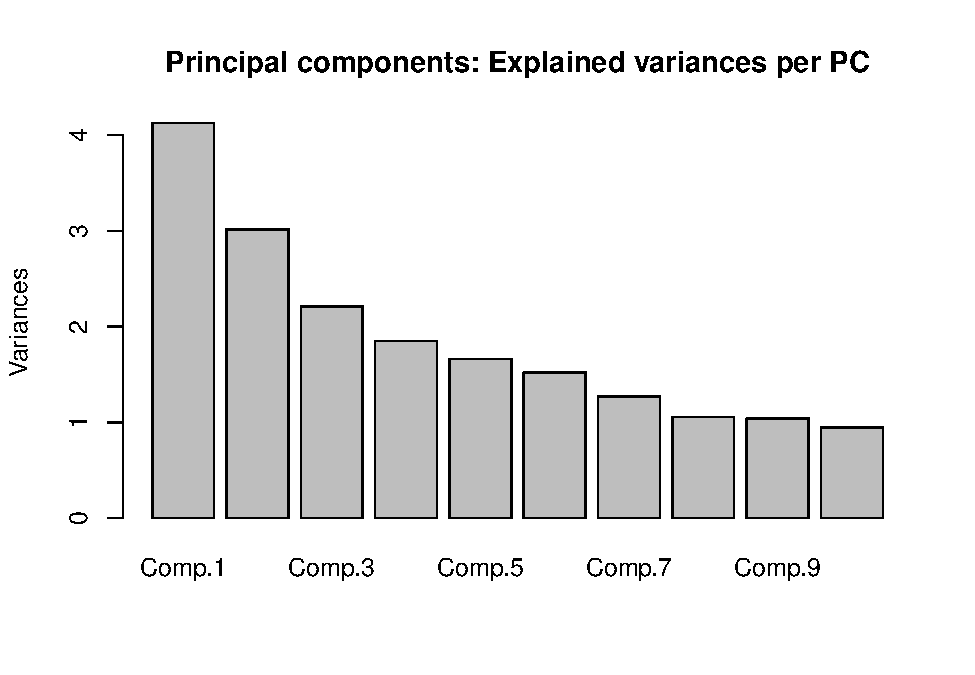
\includegraphics{Influence_factors_files/figure-latex/3.01_CA_preparation_munic-1.pdf}

\begin{Shaded}
\begin{Highlighting}[]
\CommentTok{\# write two first principal components out}
\NormalTok{pc }\OtherTok{\textless{}{-}}\NormalTok{ PC.inf.fac}\SpecialCharTok{$}\NormalTok{scores[,}\DecValTok{1}\SpecialCharTok{:}\DecValTok{2}\NormalTok{]}
\end{Highlighting}
\end{Shaded}

\hypertarget{agglomerative-clustering}{%
\subsubsection{Agglomerative
Clustering}\label{agglomerative-clustering}}

First, as described above, the approach of agglomerative clustering.
This fits best the explorative purpose of this work.

\begin{Shaded}
\begin{Highlighting}[]
\DocumentationTok{\#\# Agglomerative clustering with complete linkage}
\NormalTok{cl.inf.fac }\OtherTok{\textless{}{-}} \FunctionTok{hclust}\NormalTok{(dp, }\AttributeTok{method =} \StringTok{"complete"}\NormalTok{)}

\DocumentationTok{\#\# Show dendrogram}
\FunctionTok{plot}\NormalTok{(cl.inf.fac)}
\FunctionTok{abline}\NormalTok{(}\AttributeTok{h=}\DecValTok{14}\NormalTok{, }\AttributeTok{col=}\StringTok{"blue"}\NormalTok{)}
\end{Highlighting}
\end{Shaded}

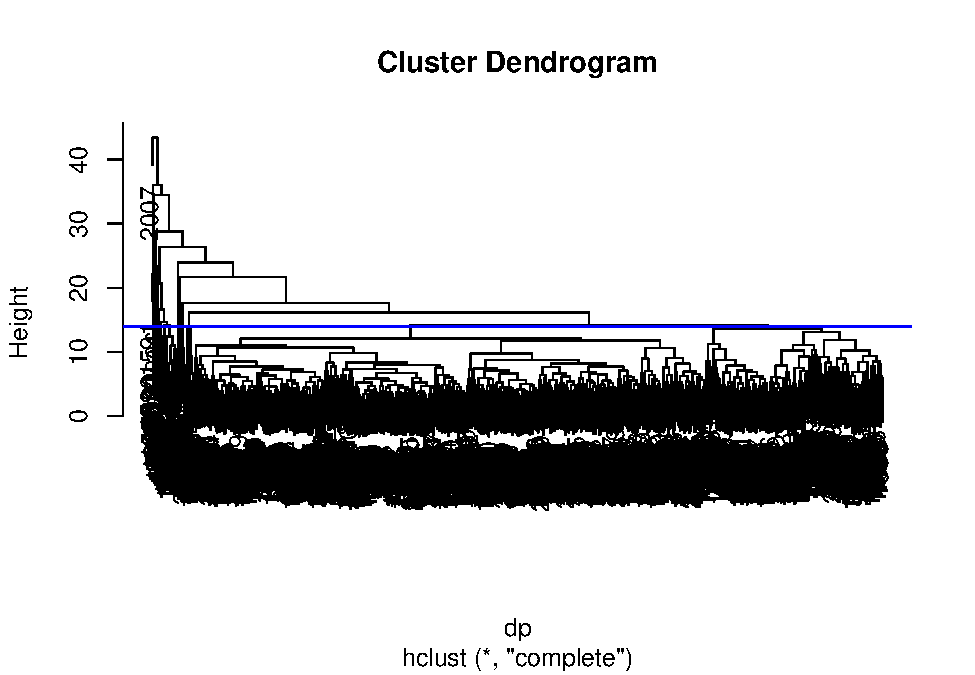
\includegraphics{Influence_factors_files/figure-latex/3.02_aggloclust_munic-1.pdf}
Out of the dendrogram, it is hard to say how many clusters would be
accurate. But it can be seen, that it's going to be very hard to
recognize clusters, as there are many clusters with only very little
observations which are cut very far up in the tree. I try to cut the
tree approximately on the drawn line so that I get at least 2 larger
groups.

\begin{Shaded}
\begin{Highlighting}[]
\DocumentationTok{\#\# Split into groups}
\NormalTok{k }\OtherTok{=} \DecValTok{18} \CommentTok{\# with 18 clusters, at least 2 big groups!}
\NormalTok{grps }\OtherTok{\textless{}{-}} \FunctionTok{cutree}\NormalTok{(cl.inf.fac, }\AttributeTok{k =}\NormalTok{ k) }


\DocumentationTok{\#\# Visualize result in PC 1 \& 2}
\FunctionTok{plot}\NormalTok{(pc, }\AttributeTok{pch =}\NormalTok{ grps, }\AttributeTok{col=}\NormalTok{grps, }\AttributeTok{lwd=}\DecValTok{2}\NormalTok{, }\AttributeTok{main=}\StringTok{"Cluster result agglomerative clustering"}\NormalTok{) }
\FunctionTok{legend}\NormalTok{(}\StringTok{"bottomright"}\NormalTok{, }\AttributeTok{legend =} \DecValTok{1}\SpecialCharTok{:}\NormalTok{k, }\AttributeTok{pch =} \DecValTok{1}\SpecialCharTok{:}\NormalTok{k, }\AttributeTok{col=}\DecValTok{1}\SpecialCharTok{:}\NormalTok{k, }\AttributeTok{bty=}\StringTok{"n"}\NormalTok{, }\AttributeTok{cex=}\FloatTok{0.85}\NormalTok{)}
\end{Highlighting}
\end{Shaded}

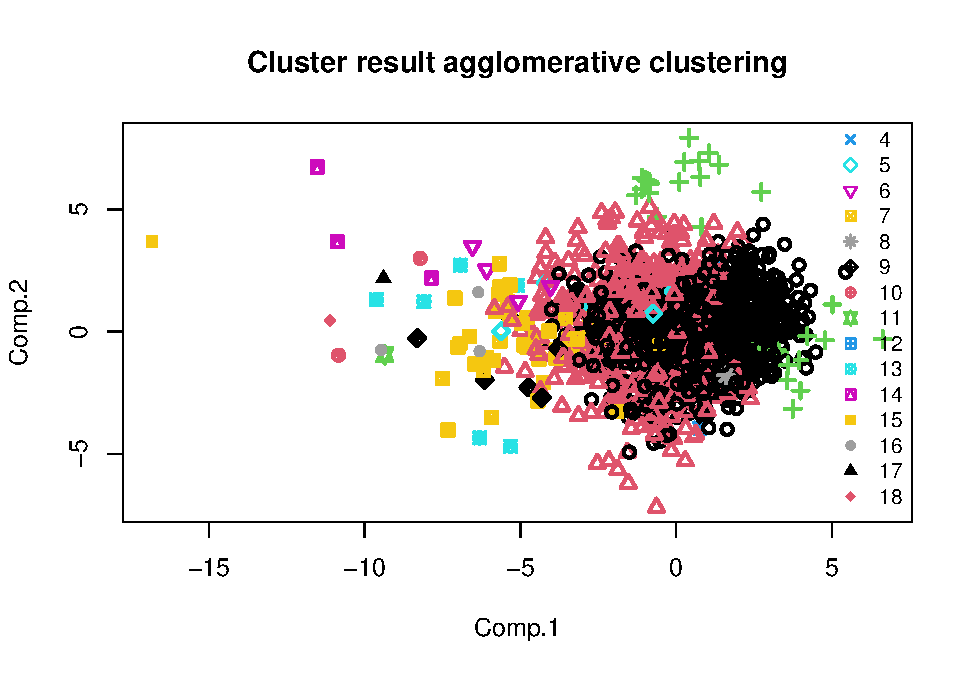
\includegraphics{Influence_factors_files/figure-latex/3.03_agglo_clust_visualize_munic-1.pdf}

\begin{Shaded}
\begin{Highlighting}[]
\DocumentationTok{\#\# Look at means of clusters / centroids}
\CommentTok{\# aggregate(cl.an.input, by=list(cluster=grps), mean)}
\end{Highlighting}
\end{Shaded}

The silhouette values can give us an evluation of the quality:

\begin{Shaded}
\begin{Highlighting}[]
\DocumentationTok{\#\# Silhouette plot from package "cluster"}
\FunctionTok{summary}\NormalTok{(cluster}\SpecialCharTok{::}\FunctionTok{silhouette}\NormalTok{(grps, dp)) }
\end{Highlighting}
\end{Shaded}

\begin{verbatim}
## Silhouette of 2058 units in 18 clusters from silhouette.default(x = grps, dist = dp) :
##  Cluster sizes and average silhouette widths:
##        1437         499          30           2           9           4 
##  0.17211056 -0.05953620  0.03479200  0.16262482  0.25126546  0.14805391 
##          41           5           8           2           2           4 
##  0.03999173  0.21953811  0.16017068  0.39476326 -0.08194178  0.40659218 
##           6           3           1           3           1           1 
##  0.13357709  0.16971259  0.00000000  0.23201081  0.00000000  0.00000000 
## Individual silhouette widths:
##    Min. 1st Qu.  Median    Mean 3rd Qu.    Max. 
## -0.2762  0.0212  0.1486  0.1118  0.2064  0.5811
\end{verbatim}

Due to the amount of data, the silhouette plot is not shown properly,
but the average silhouette width of 0.11 is very low, making the
classification relatively bad.

\hypertarget{k-means-clustering}{%
\subsubsection{k-means clustering}\label{k-means-clustering}}

The second method is k-means clustering, in which it must be defined
from the beginning how many clusters there should eventually be.

\begin{Shaded}
\begin{Highlighting}[]
\CommentTok{\# k{-}means}

\DocumentationTok{\#\# Choose number of clusters k with scree plot}
\NormalTok{nr }\OtherTok{\textless{}{-}} \DecValTok{12}
\NormalTok{wss }\OtherTok{\textless{}{-}} \FunctionTok{rep}\NormalTok{(}\DecValTok{0}\NormalTok{, nr)}
\ControlFlowTok{for}\NormalTok{ (i }\ControlFlowTok{in} \DecValTok{1}\SpecialCharTok{:}\NormalTok{nr) wss[i] }\OtherTok{\textless{}{-}} \FunctionTok{sum}\NormalTok{(}\FunctionTok{kmeans}\NormalTok{(cl.an.input[,}\DecValTok{2}\SpecialCharTok{:}\DecValTok{25}\NormalTok{], }\AttributeTok{centers =}\NormalTok{ i, }\AttributeTok{nstart =} \DecValTok{20}\NormalTok{)}\SpecialCharTok{$}\NormalTok{withinss)}
\FunctionTok{par}\NormalTok{(}\AttributeTok{mfrow =} \FunctionTok{c}\NormalTok{(}\DecValTok{1}\NormalTok{,}\DecValTok{1}\NormalTok{))}
\FunctionTok{plot}\NormalTok{(}\DecValTok{1}\SpecialCharTok{:}\NormalTok{nr, wss, }\AttributeTok{type =} \StringTok{"b"}\NormalTok{, }\AttributeTok{xlab =} \StringTok{"Number of groups"}\NormalTok{, }\AttributeTok{ylab =} \StringTok{"Within groups sum of squares"}\NormalTok{)}
\end{Highlighting}
\end{Shaded}

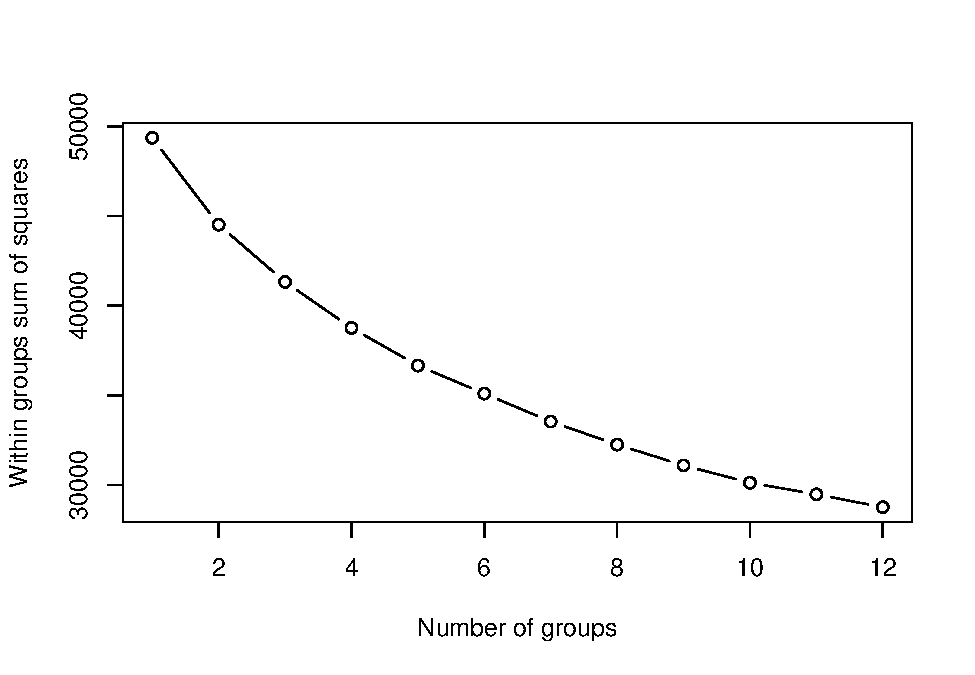
\includegraphics{Influence_factors_files/figure-latex/3.05_kmeans1_munic-1.pdf}
No kink can be detected here unfortunately. With this scree plot, there
is no good basis for a decision here, so everything from 1-10 is tried
out and the corresponding silhouette values are compared with each
other.

\begin{Shaded}
\begin{Highlighting}[]
\NormalTok{seed }\OtherTok{=} \DecValTok{123}
\ControlFlowTok{for}\NormalTok{(k }\ControlFlowTok{in} \DecValTok{2}\SpecialCharTok{:}\DecValTok{10}\NormalTok{) \{}
\NormalTok{  seed }\OtherTok{=} \DecValTok{123}
  \DocumentationTok{\#\# k{-}means with 3{-}10 centers}
\NormalTok{  ckm }\OtherTok{\textless{}{-}} \FunctionTok{kmeans}\NormalTok{(cl.an.input[,}\DecValTok{2}\SpecialCharTok{:}\DecValTok{25}\NormalTok{], }\AttributeTok{centers =}\NormalTok{ k, }\AttributeTok{nstart =} \DecValTok{10}\NormalTok{)}
\NormalTok{  grpsKM }\OtherTok{\textless{}{-}}\NormalTok{ ckm}\SpecialCharTok{$}\NormalTok{cluster}

  \DocumentationTok{\#\# Silhouette Summary}
  \FunctionTok{print}\NormalTok{(}\FunctionTok{paste}\NormalTok{(}\StringTok{"k means clustering with "}\NormalTok{, k, }\StringTok{"clusters: Individual silhouette widths:"}\NormalTok{))}
  \FunctionTok{print}\NormalTok{(}\FunctionTok{summary}\NormalTok{(}\FunctionTok{silhouette}\NormalTok{(grpsKM, dp))[}\DecValTok{1}\NormalTok{])}
  
\NormalTok{\}}
\end{Highlighting}
\end{Shaded}

\begin{verbatim}
## [1] "k means clustering with  2 clusters: Individual silhouette widths:"
## $si.summary
##    Min. 1st Qu.  Median    Mean 3rd Qu.    Max. 
## -0.2325  0.1842  0.2920  0.2258  0.3429  0.4392 
## 
## [1] "k means clustering with  3 clusters: Individual silhouette widths:"
## $si.summary
##     Min.  1st Qu.   Median     Mean  3rd Qu.     Max. 
## -0.26878  0.02135  0.08763  0.07922  0.15548  0.30615 
## 
## [1] "k means clustering with  4 clusters: Individual silhouette widths:"
## $si.summary
##     Min.  1st Qu.   Median     Mean  3rd Qu.     Max. 
## -0.31588  0.03105  0.08946  0.08690  0.15529  0.30917 
## 
## [1] "k means clustering with  5 clusters: Individual silhouette widths:"
## $si.summary
##     Min.  1st Qu.   Median     Mean  3rd Qu.     Max. 
## -0.22250  0.03067  0.09175  0.09004  0.16095  0.32863 
## 
## [1] "k means clustering with  6 clusters: Individual silhouette widths:"
## $si.summary
##     Min.  1st Qu.   Median     Mean  3rd Qu.     Max. 
## -0.41067  0.03051  0.09175  0.08766  0.15606  0.29885 
## 
## [1] "k means clustering with  7 clusters: Individual silhouette widths:"
## $si.summary
##     Min.  1st Qu.   Median     Mean  3rd Qu.     Max. 
## -0.25667  0.02002  0.10010  0.08802  0.16219  0.41116 
## 
## [1] "k means clustering with  8 clusters: Individual silhouette widths:"
## $si.summary
##     Min.  1st Qu.   Median     Mean  3rd Qu.     Max. 
## -0.26396  0.03166  0.08642  0.08897  0.15309  0.41460 
## 
## [1] "k means clustering with  9 clusters: Individual silhouette widths:"
## $si.summary
##     Min.  1st Qu.   Median     Mean  3rd Qu.     Max. 
## -0.25885  0.02140  0.07337  0.07410  0.13139  0.41240 
## 
## [1] "k means clustering with  10 clusters: Individual silhouette widths:"
## $si.summary
##     Min.  1st Qu.   Median     Mean  3rd Qu.     Max. 
## -0.22411  0.03370  0.09173  0.09246  0.15916  0.40185
\end{verbatim}

Possibilities are k=2 or k=6 here:

\begin{Shaded}
\begin{Highlighting}[]
\DocumentationTok{\#\# k{-}means with 2 centers}
\NormalTok{ckm2 }\OtherTok{\textless{}{-}} \FunctionTok{kmeans}\NormalTok{(cl.an.input[,}\DecValTok{2}\SpecialCharTok{:}\DecValTok{25}\NormalTok{], }\AttributeTok{centers =} \DecValTok{2}\NormalTok{, }\AttributeTok{nstart =} \DecValTok{10}\NormalTok{)}
\NormalTok{grpsKM2}\OtherTok{\textless{}{-}}\NormalTok{ ckm2}\SpecialCharTok{$}\NormalTok{cluster}

\DocumentationTok{\#\# k{-}means with 6 centers}
\NormalTok{ckm6 }\OtherTok{\textless{}{-}} \FunctionTok{kmeans}\NormalTok{(cl.an.input[,}\DecValTok{2}\SpecialCharTok{:}\DecValTok{25}\NormalTok{], }\AttributeTok{centers =} \DecValTok{6}\NormalTok{, }\AttributeTok{nstart =} \DecValTok{10}\NormalTok{)}
\NormalTok{grpsKM6}\OtherTok{\textless{}{-}}\NormalTok{ ckm6}\SpecialCharTok{$}\NormalTok{cluster}
\end{Highlighting}
\end{Shaded}

\hypertarget{gaussian-mixture-model}{%
\subsubsection{Gaussian mixture model}\label{gaussian-mixture-model}}

The Guassian mixture model makes the assumption that there is a
statistical model behind the data. In this case, that is also partly the
case, which makes it worthwhile to try it out.

\begin{Shaded}
\begin{Highlighting}[]
\DocumentationTok{\#\#\#\#\#\#\#\#\#\#\#\#\#\#\#\#\#\#\#\#\#\#\#\#\#\#\#\#\#\#\#}
\DocumentationTok{\#\# Gaussian Mixture Models \#\#\#\#}
\DocumentationTok{\#\#\#\#\#\#\#\#\#\#\#\#\#\#\#\#\#\#\#\#\#\#\#\#\#\#\#\#\#\#\#}
\NormalTok{mc }\OtherTok{\textless{}{-}} \FunctionTok{Mclust}\NormalTok{(cl.an.input[,}\DecValTok{2}\SpecialCharTok{:}\DecValTok{25}\NormalTok{]) }\CommentTok{\# takes long time!}
\FunctionTok{table}\NormalTok{(mc}\SpecialCharTok{$}\NormalTok{classification)}
\end{Highlighting}
\end{Shaded}

\begin{verbatim}
## 
##   1   2   3   4   5   6   7 
## 307 166 611 459 293 143  79
\end{verbatim}

With this approach, 7 classes were built here.

\hypertarget{dbscan}{%
\subsubsection{DBSCAN}\label{dbscan}}

The last approach is the ``Density-Based Spatial Clustering of
Applications with Noise''. Two characteristics distinguish this
procedure: On the one hand, it is density-based, i.e.~it sees points
that are close to each other from a density-based perspective as
belonging together. On the other hand, it classifies points that lie
outside the recognised clusters as ``noise'' points. This means that the
method can deal well with outliers by simply deleting them from the
cluster analysis. In the case of the many municipalities, there are
certainly outliers, which also makes the procedure make sense here.

\begin{Shaded}
\begin{Highlighting}[]
\CommentTok{\# DBSCAN}
\FunctionTok{kNNdistplot}\NormalTok{(cl.an.input[,}\DecValTok{2}\SpecialCharTok{:}\DecValTok{25}\NormalTok{], }\AttributeTok{k =} \DecValTok{26}\NormalTok{) }\DocumentationTok{\#\# {-}\textgreater{} k = dim + 1; eps value = 6 (sharp increase)}
\FunctionTok{abline}\NormalTok{(}\AttributeTok{h=}\DecValTok{6}\NormalTok{, }\AttributeTok{col =} \StringTok{"red"}\NormalTok{, }\AttributeTok{lty=}\DecValTok{2}\NormalTok{)}
\end{Highlighting}
\end{Shaded}

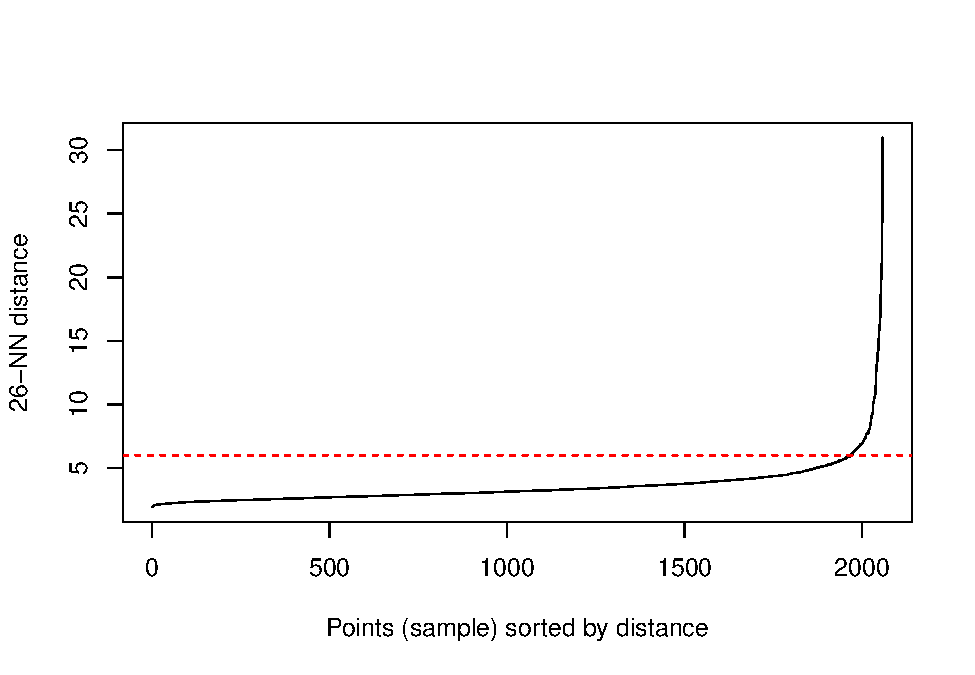
\includegraphics{Influence_factors_files/figure-latex/3.09_dbscan1_munic-1.pdf}

\begin{Shaded}
\begin{Highlighting}[]
\CommentTok{\# setting parameters according to minPts = k and eps = sharp increase}
\NormalTok{minPts}\OtherTok{=}\DecValTok{26} \CommentTok{\# = k}
\NormalTok{eps}\OtherTok{=}\DecValTok{6} \CommentTok{\# cutting line above}
\NormalTok{dbs }\OtherTok{\textless{}{-}} \FunctionTok{dbscan}\NormalTok{(cl.an.input[,}\DecValTok{2}\SpecialCharTok{:}\DecValTok{25}\NormalTok{], }\AttributeTok{eps =}\NormalTok{ eps, }\AttributeTok{minPts =}\NormalTok{ minPts)}
\FunctionTok{max}\NormalTok{(dbs}\SpecialCharTok{$}\NormalTok{cluster) }\CommentTok{\# 1}
\end{Highlighting}
\end{Shaded}

\begin{verbatim}
## [1] 1
\end{verbatim}

Only 1 cluster is present here, alternate values of minPts and eps to
get another amount of clusters:

\begin{Shaded}
\begin{Highlighting}[]
\CommentTok{\# Searching for better parameters:}
\DocumentationTok{\#\# For eps value (i), only values from 1 to 5 are tested, because higher values }
\DocumentationTok{\#\# always lead to only one cluster at the end.}

\CommentTok{\# For minPts, the range from 2 to 5 is tested. 1 would lead to as many clusters }
\CommentTok{\# as points are and for more than 5, only one cluster can be obtained. }

\ControlFlowTok{for}\NormalTok{(i }\ControlFlowTok{in}\NormalTok{ (}\DecValTok{1}\SpecialCharTok{:}\DecValTok{5}\NormalTok{)) \{}
  
  \ControlFlowTok{for}\NormalTok{(j }\ControlFlowTok{in}\NormalTok{ (}\DecValTok{2}\SpecialCharTok{:}\DecValTok{5}\NormalTok{)) \{}

\NormalTok{    dbs }\OtherTok{\textless{}{-}} \FunctionTok{dbscan}\NormalTok{(cl.an.input[,}\DecValTok{2}\SpecialCharTok{:}\DecValTok{25}\NormalTok{], }\AttributeTok{eps =}\NormalTok{ i, }\AttributeTok{minPts =}\NormalTok{ j)}

    \FunctionTok{print}\NormalTok{(}\FunctionTok{paste}\NormalTok{(}\StringTok{"minPts:"}\NormalTok{, j, }\StringTok{"; eps: "}\NormalTok{, i, }\StringTok{"; nr. of clusters: "}\NormalTok{, }\FunctionTok{max}\NormalTok{(dbs}\SpecialCharTok{$}\NormalTok{cluster))) }\CommentTok{\# 1}
    \FunctionTok{print}\NormalTok{(}\FunctionTok{table}\NormalTok{(dbs}\SpecialCharTok{$}\NormalTok{cluster))}
\NormalTok{  \}}

\NormalTok{\}}
\end{Highlighting}
\end{Shaded}

\begin{verbatim}
## [1] "minPts: 2 ; eps:  1 ; nr. of clusters:  0"
## 
##    0 
## 2058 
## [1] "minPts: 3 ; eps:  1 ; nr. of clusters:  0"
## 
##    0 
## 2058 
## [1] "minPts: 4 ; eps:  1 ; nr. of clusters:  0"
## 
##    0 
## 2058 
## [1] "minPts: 5 ; eps:  1 ; nr. of clusters:  0"
## 
##    0 
## 2058 
## [1] "minPts: 2 ; eps:  2 ; nr. of clusters:  83"
## 
##    0    1    2    3    4    5    6    7    8    9   10   11   12   13   14   15 
## 1231    4  585    3    5    2    2    2    2    2    2    2    3    2    2    2 
##   16   17   18   19   20   21   22   23   24   25   26   27   28   29   30   31 
##    9    3    2    6    2    2    3    2    4    5    2    2    3    3    5    2 
##   32   33   34   35   36   37   38   39   40   41   42   43   44   45   46   47 
##   11    5    2    3    4    2    2    3    2    2    2    2    3    2    3    2 
##   48   49   50   51   52   53   54   55   56   57   58   59   60   61   62   63 
##    2    2    3    2    2    4    2    2    2    2    3    2    4   14    2    4 
##   64   65   66   67   68   69   70   71   72   73   74   75   76   77   78   79 
##    4    3    2    2    2    2    2    3    6    2    3    2    2    2    3    2 
##   80   81   82   83 
##    2    2    2    2 
## [1] "minPts: 3 ; eps:  2 ; nr. of clusters:  33"
## 
##    0    1    2    3    4    5    6    7    8    9   10   11   12   13   14   15 
## 1331    4  585    5    3    4    5    9    3    3    3   11    5    6    3    3 
##   16   17   18   19   20   21   22   23   24   25   26   27   28   29   30   31 
##    3    3    3    3    4    4    3    3   14    4    4    3    3    6    4    3 
##   32   33 
##    3    5 
## [1] "minPts: 4 ; eps:  2 ; nr. of clusters:  17"
## 
##    0    1    2    3    4    5    6    7    8    9   10   11   12   13   14   15 
## 1443  534    5    4    8    3   11    6    4    4    4    4    6    3    4    6 
##   16   17 
##    4    5 
## [1] "minPts: 5 ; eps:  2 ; nr. of clusters:  5"
## 
##    0    1    2    3    4    5 
## 1533  496    5    7   11    6 
## [1] "minPts: 2 ; eps:  3 ; nr. of clusters:  16"
## 
##    0    1    2    3    4    5    6    7    8    9   10   11   12   13   14   15 
##  353 1667    2    3    2    2    2    2    4    2    4    3    3    2    3    2 
##   16 
##    2 
## [1] "minPts: 3 ; eps:  3 ; nr. of clusters:  7"
## 
##    0    1    2    3    4    5    6    7 
##  371 1667    3    4    3    3    4    3 
## [1] "minPts: 4 ; eps:  3 ; nr. of clusters:  1"
## 
##    0    1 
##  397 1661 
## [1] "minPts: 5 ; eps:  3 ; nr. of clusters:  1"
## 
##    0    1 
##  411 1647 
## [1] "minPts: 2 ; eps:  4 ; nr. of clusters:  3"
## 
##    0    1    2    3 
##  132 1922    2    2 
## [1] "minPts: 3 ; eps:  4 ; nr. of clusters:  1"
## 
##    0    1 
##  136 1922 
## [1] "minPts: 4 ; eps:  4 ; nr. of clusters:  1"
## 
##    0    1 
##  140 1918 
## [1] "minPts: 5 ; eps:  4 ; nr. of clusters:  1"
## 
##    0    1 
##  142 1916 
## [1] "minPts: 2 ; eps:  5 ; nr. of clusters:  2"
## 
##    0    1    2 
##   59 1997    2 
## [1] "minPts: 3 ; eps:  5 ; nr. of clusters:  1"
## 
##    0    1 
##   61 1997 
## [1] "minPts: 4 ; eps:  5 ; nr. of clusters:  1"
## 
##    0    1 
##   62 1996 
## [1] "minPts: 5 ; eps:  5 ; nr. of clusters:  1"
## 
##    0    1 
##   64 1994
\end{verbatim}

DBSCAN works very poorly here. Either practically all points are noise
points or in a cluster, there is nothing in between.

\hypertarget{comparison-of-different-approaches}{%
\subsubsection{Comparison of different
approaches}\label{comparison-of-different-approaches}}

\begin{Shaded}
\begin{Highlighting}[]
\DocumentationTok{\#\# PLOT CLUSTER CALSSES ON PC 1 \& 2 }

\FunctionTok{par}\NormalTok{(}\AttributeTok{mfrow=}\FunctionTok{c}\NormalTok{(}\DecValTok{2}\NormalTok{,}\DecValTok{2}\NormalTok{), }\AttributeTok{mar=}\FunctionTok{c}\NormalTok{(}\DecValTok{2}\NormalTok{,}\DecValTok{2}\NormalTok{,}\FloatTok{1.5}\NormalTok{,}\DecValTok{1}\NormalTok{))}

\CommentTok{\# Gaussian Mixture model}
\FunctionTok{plot}\NormalTok{(pc, }\AttributeTok{pch =}\NormalTok{ mc}\SpecialCharTok{$}\NormalTok{classification, }\AttributeTok{col =}\NormalTok{ mc}\SpecialCharTok{$}\NormalTok{classification, }
     \AttributeTok{main=}\StringTok{"Gaussian Mixture Model (4 clusters)"}\NormalTok{)}
\FunctionTok{legend}\NormalTok{(}\StringTok{"bottomright"}\NormalTok{, }\AttributeTok{legend =} \DecValTok{1}\SpecialCharTok{:}\DecValTok{4}\NormalTok{, }\AttributeTok{pch =} \DecValTok{1}\SpecialCharTok{:}\DecValTok{4}\NormalTok{, }\AttributeTok{col=}\DecValTok{1}\SpecialCharTok{:}\DecValTok{4}\NormalTok{, }\AttributeTok{bty=}\StringTok{"n"}\NormalTok{)}

\CommentTok{\# K{-}means with 2 clusters}
\FunctionTok{plot}\NormalTok{(pc, }\AttributeTok{pch =}\NormalTok{ grpsKM2, }\AttributeTok{col=}\NormalTok{grpsKM2, }\AttributeTok{main=}\StringTok{"K{-}means (2 clusters)"}\NormalTok{)}
\FunctionTok{legend}\NormalTok{(}\StringTok{"bottomright"}\NormalTok{, }\AttributeTok{legend =} \DecValTok{1}\SpecialCharTok{:}\DecValTok{2}\NormalTok{, }\AttributeTok{pch =} \DecValTok{1}\SpecialCharTok{:}\DecValTok{2}\NormalTok{, }\AttributeTok{col=}\DecValTok{1}\SpecialCharTok{:}\DecValTok{2}\NormalTok{, }\AttributeTok{bty=}\StringTok{"n"}\NormalTok{)}

\CommentTok{\# K{-}means with 6 clusters}
\FunctionTok{plot}\NormalTok{(pc, }\AttributeTok{pch =}\NormalTok{ grpsKM6, }\AttributeTok{col=}\NormalTok{grpsKM6, }\AttributeTok{main=}\StringTok{"K{-}means (6 clusters)"}\NormalTok{)}
\FunctionTok{legend}\NormalTok{(}\StringTok{"bottomright"}\NormalTok{, }\AttributeTok{legend =} \DecValTok{1}\SpecialCharTok{:}\DecValTok{6}\NormalTok{, }\AttributeTok{pch =} \DecValTok{1}\SpecialCharTok{:}\DecValTok{6}\NormalTok{, }\AttributeTok{col=}\DecValTok{1}\SpecialCharTok{:}\DecValTok{5}\NormalTok{, }\AttributeTok{bty=}\StringTok{"n"}\NormalTok{)}

\CommentTok{\# Agglomerative clustering}
\FunctionTok{plot}\NormalTok{(pc, }\AttributeTok{pch =}\NormalTok{ grps, }\AttributeTok{col=}\NormalTok{grps, }\AttributeTok{main=}\StringTok{"Agglomerative clustering (18 clusters)"}\NormalTok{)}
\FunctionTok{legend}\NormalTok{(}\StringTok{"bottomright"}\NormalTok{, }\AttributeTok{legend =} \DecValTok{1}\SpecialCharTok{:}\DecValTok{18}\NormalTok{, }\AttributeTok{pch =} \DecValTok{1}\SpecialCharTok{:}\DecValTok{18}\NormalTok{, }\AttributeTok{col=}\DecValTok{1}\SpecialCharTok{:}\DecValTok{18}\NormalTok{, }\AttributeTok{bty=}\StringTok{"n"}\NormalTok{, }\AttributeTok{cex=}\FloatTok{0.5}\NormalTok{)}
\end{Highlighting}
\end{Shaded}

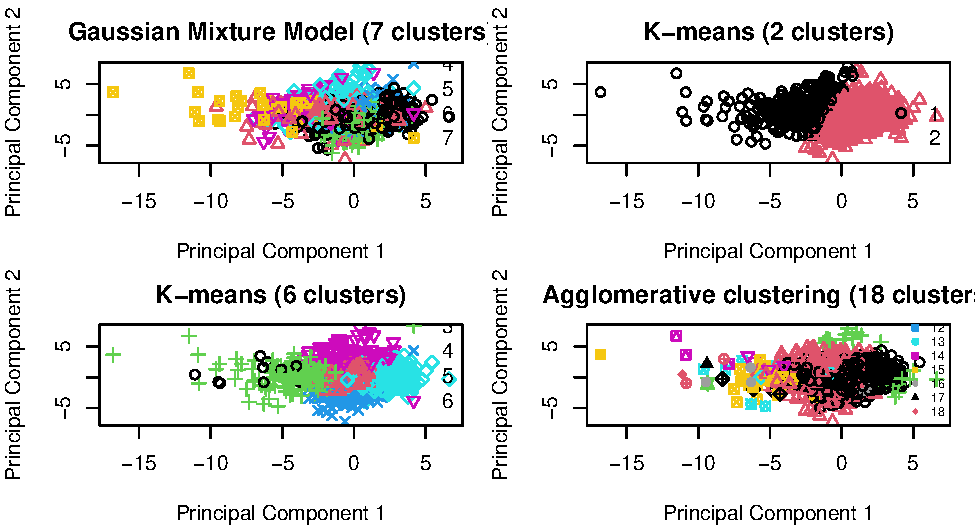
\includegraphics{Influence_factors_files/figure-latex/3.11_ca_comparison_munic-1.pdf}

\begin{Shaded}
\begin{Highlighting}[]
\DocumentationTok{\#\# SILHOUETTE PLOTS \#\#}

\DocumentationTok{\#\# Reduce number of data to see a sample of the whole dataset}

\CommentTok{\# classifications}
\NormalTok{grps.ss }\OtherTok{\textless{}{-}}\NormalTok{ grps[}\DecValTok{1}\SpecialCharTok{:}\DecValTok{200}\NormalTok{]}
\NormalTok{mc.ss }\OtherTok{\textless{}{-}}\NormalTok{ mc}\SpecialCharTok{$}\NormalTok{classification[}\DecValTok{1}\SpecialCharTok{:}\DecValTok{200}\NormalTok{]}
\NormalTok{grpsKM2.ss }\OtherTok{\textless{}{-}}\NormalTok{ grpsKM2[}\DecValTok{1}\SpecialCharTok{:}\DecValTok{200}\NormalTok{]}
\NormalTok{grpsKM6.ss }\OtherTok{\textless{}{-}}\NormalTok{ grpsKM6[}\DecValTok{1}\SpecialCharTok{:}\DecValTok{200}\NormalTok{]}

\CommentTok{\# distance table}
\NormalTok{dp.ss }\OtherTok{\textless{}{-}} \FunctionTok{dist}\NormalTok{(cl.an.input[}\DecValTok{1}\SpecialCharTok{:}\DecValTok{200}\NormalTok{,}\DecValTok{2}\SpecialCharTok{:}\DecValTok{25}\NormalTok{]) }\DocumentationTok{\#\# Euclidean}

\CommentTok{\# Silhouette Plot from package "cluster"}
\FunctionTok{par}\NormalTok{(}\AttributeTok{mfrow=}\FunctionTok{c}\NormalTok{(}\DecValTok{1}\NormalTok{,}\DecValTok{2}\NormalTok{), }\AttributeTok{mar=}\FunctionTok{c}\NormalTok{(}\DecValTok{5}\NormalTok{,}\DecValTok{4}\NormalTok{,}\DecValTok{4}\NormalTok{,}\DecValTok{2}\NormalTok{))}

\FunctionTok{plot}\NormalTok{(}\FunctionTok{silhouette}\NormalTok{(grps.ss, dp.ss, }\AttributeTok{cex=}\FloatTok{0.8}\NormalTok{), }\AttributeTok{main=}\StringTok{"Agglomerative clustering"}\NormalTok{)}
\FunctionTok{plot}\NormalTok{(}\FunctionTok{silhouette}\NormalTok{(grpsKM2.ss, dp.ss), }\AttributeTok{main=}\StringTok{"k{-}means clustering (k=2)"}\NormalTok{)}
\end{Highlighting}
\end{Shaded}

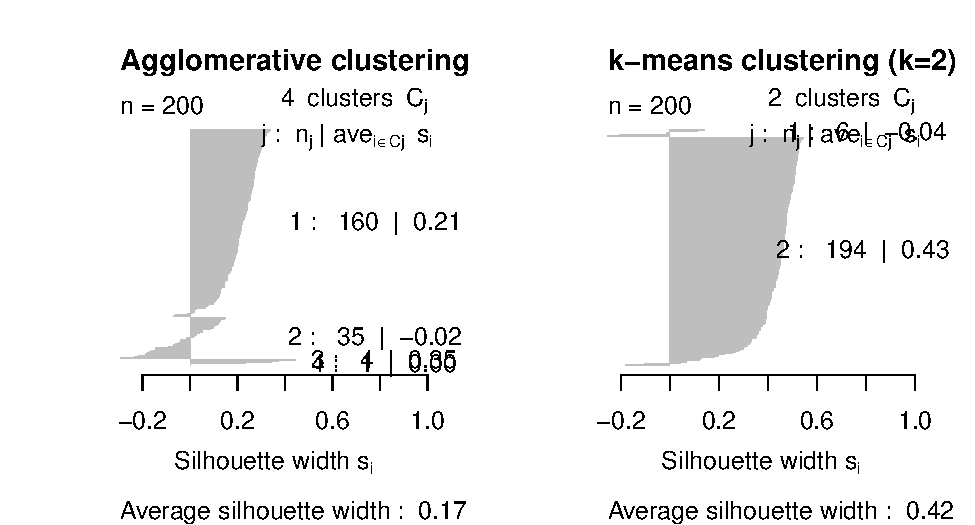
\includegraphics{Influence_factors_files/figure-latex/3.11_ca_comparison_munic-2.pdf}

\begin{Shaded}
\begin{Highlighting}[]
\FunctionTok{plot}\NormalTok{(}\FunctionTok{silhouette}\NormalTok{(grpsKM6.ss, dp.ss), }\AttributeTok{main=}\StringTok{"k{-}means clustering (k=6)"}\NormalTok{)}
\FunctionTok{plot}\NormalTok{(}\FunctionTok{silhouette}\NormalTok{(mc.ss, dp.ss), }\AttributeTok{main=}\StringTok{"Gaussian mixture model"}\NormalTok{)}
\end{Highlighting}
\end{Shaded}

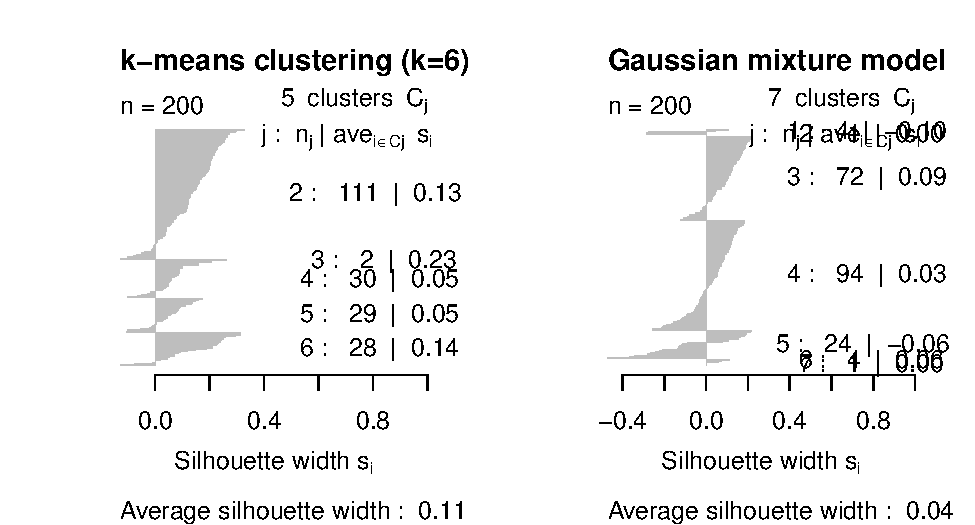
\includegraphics{Influence_factors_files/figure-latex/3.11_ca_comparison_munic-3.pdf}

\begin{Shaded}
\begin{Highlighting}[]
\DocumentationTok{\#\# GROUPS REPRESENTING LANGUAGE REGIONS}

\NormalTok{ca.aggl.lan }\OtherTok{\textless{}{-}} \FunctionTok{data.frame}\NormalTok{(}\AttributeTok{cls =}\NormalTok{ grps, }\AttributeTok{lang =}\NormalTok{ cl.an.input[,}\DecValTok{1}\NormalTok{])}
\FunctionTok{table}\NormalTok{(ca.aggl.lan)}
\end{Highlighting}
\end{Shaded}

\begin{verbatim}
##     lang
## cls   de  fr  it  rm
##   1  895 463  66  13
##   2  337 109  31  22
##   3   11  19   0   0
##   4    2   0   0   0
##   5    5   4   0   0
##   6    4   0   0   0
##   7   17   2  15   7
##   8    3   2   0   0
##   9    6   0   2   0
##   10   1   1   0   0
##   11   1   0   1   0
##   12   3   0   0   1
##   13   3   0   2   1
##   14   2   0   1   0
##   15   0   0   1   0
##   16   3   0   0   0
##   17   1   0   0   0
##   18   1   0   0   0
\end{verbatim}

\begin{Shaded}
\begin{Highlighting}[]
\NormalTok{ca.km2.lan }\OtherTok{\textless{}{-}} \FunctionTok{data.frame}\NormalTok{(}\AttributeTok{cls =}\NormalTok{ grpsKM2, }\AttributeTok{lang =}\NormalTok{ cl.an.input[,}\DecValTok{1}\NormalTok{])}
\FunctionTok{table}\NormalTok{(ca.km2.lan)}
\end{Highlighting}
\end{Shaded}

\begin{verbatim}
##    lang
## cls   de   fr   it   rm
##   1  241   85   95   36
##   2 1054  515   24    8
\end{verbatim}

\begin{Shaded}
\begin{Highlighting}[]
\NormalTok{ca.km6.lan }\OtherTok{\textless{}{-}} \FunctionTok{data.frame}\NormalTok{(}\AttributeTok{cls =}\NormalTok{ grpsKM6, }\AttributeTok{lang =}\NormalTok{ cl.an.input[,}\DecValTok{1}\NormalTok{])}
\FunctionTok{table}\NormalTok{(ca.km6.lan)}
\end{Highlighting}
\end{Shaded}

\begin{verbatim}
##    lang
## cls  de  fr  it  rm
##   1   9   0   1   0
##   2 541 123  40  10
##   3  93  30  58  30
##   4 412  20   3   0
##   5 102 333   7   1
##   6 138  94  10   3
\end{verbatim}

\begin{Shaded}
\begin{Highlighting}[]
\NormalTok{ca.mc.lan }\OtherTok{\textless{}{-}} \FunctionTok{data.frame}\NormalTok{(}\AttributeTok{cls =}\NormalTok{ mc}\SpecialCharTok{$}\NormalTok{classification, }\AttributeTok{lang =}\NormalTok{ cl.an.input[,}\DecValTok{1}\NormalTok{])}
\FunctionTok{table}\NormalTok{(ca.mc.lan)}
\end{Highlighting}
\end{Shaded}

\begin{verbatim}
##    lang
## cls  de  fr  it  rm
##   1  64 237   0   6
##   2  73  66  16  11
##   3 504 107   0   0
##   4 366  92   0   1
##   5 149  58  80   6
##   6  78  31  18  16
##   7  61   9   5   4
\end{verbatim}

The outcome of the cluster analysis on the municipality level is, that
it is not applicable, as the huge amount of data is too wide-spreaded.
The best approach is reached with a k-means clustering with k=6. This
can be written in a separate table to look at it graphically.

\hypertarget{exporting-enriched-data}{%
\subsubsection{Exporting enriched data}\label{exporting-enriched-data}}

The generated clusters can now be written into a table together with the
relevant influencing factors, which can then be used for the
distribution of shares and graphical analysis with Tableau.

\begin{Shaded}
\begin{Highlighting}[]
\CommentTok{\# filtering out language (loading separate) and interaction terms}
\NormalTok{d.share.clust }\OtherTok{\textless{}{-}}\NormalTok{ d.share[,}\FunctionTok{c}\NormalTok{(}\StringTok{"language"}\NormalTok{, }\FunctionTok{rownames}\NormalTok{(inf\_factors)[}\FunctionTok{c}\NormalTok{(}\DecValTok{2}\SpecialCharTok{:}\DecValTok{17}\NormalTok{, }\DecValTok{21}\NormalTok{, }\DecValTok{24}\SpecialCharTok{:}\DecValTok{29}\NormalTok{, }\DecValTok{31}\NormalTok{)])]}

\NormalTok{d.share.clust[}\StringTok{"k\_cluster"}\NormalTok{] }\OtherTok{=}\NormalTok{ grpsKM6}

\NormalTok{d.share.clust[}\StringTok{"GA\_share"}\NormalTok{] }\OtherTok{=}\NormalTok{ d.share}\SpecialCharTok{$}\NormalTok{GA\_share}
\NormalTok{d.share.clust[}\StringTok{"HTA\_share"}\NormalTok{] }\OtherTok{=}\NormalTok{ d.share}\SpecialCharTok{$}\NormalTok{HTA\_share}
\NormalTok{d.share.clust[}\StringTok{"FNT\_share"}\NormalTok{] }\OtherTok{=}\NormalTok{ d.share}\SpecialCharTok{$}\NormalTok{FNT\_share}

\NormalTok{d.share.clust[}\StringTok{"BFS\_Nr"}\NormalTok{] }\OtherTok{=}\NormalTok{ d.share}\SpecialCharTok{$}\NormalTok{BFS\_Nr}
\NormalTok{d.share.clust[}\StringTok{"municipality"}\NormalTok{] }\OtherTok{=}\NormalTok{ d.share}\SpecialCharTok{$}\NormalTok{municipality}
\NormalTok{d.share.clust[}\StringTok{"canton"}\NormalTok{] }\OtherTok{=}\NormalTok{ d.share}\SpecialCharTok{$}\NormalTok{canton}
\NormalTok{d.share.clust[}\StringTok{"language"}\NormalTok{] }\OtherTok{=}\NormalTok{ d.share}\SpecialCharTok{$}\NormalTok{language}

\DocumentationTok{\#\#\# 1. look at values for influence factors per cluster for k=6}
\DocumentationTok{\#\#\# 2. print out values in a table for tableau}
\DocumentationTok{\#\#\# 3. write text new above!}
\DocumentationTok{\#\#\# 4. Same approach for cluster analysis canton}
\end{Highlighting}
\end{Shaded}

\begin{Shaded}
\begin{Highlighting}[]
\FunctionTok{write.csv}\NormalTok{(d.share.clust, }\AttributeTok{file=}\StringTok{"influence\_factors\_with\_CA.csv"}\NormalTok{)}
\end{Highlighting}
\end{Shaded}

\hypertarget{share-distribution-of-ga-hta-and-fnt-for-clusters}{%
\subsubsection{Share distribution of GA, HTA and FNT for
clusters}\label{share-distribution-of-ga-hta-and-fnt-for-clusters}}

\begin{Shaded}
\begin{Highlighting}[]
\FunctionTok{par}\NormalTok{(}\AttributeTok{mfrow=}\FunctionTok{c}\NormalTok{(}\DecValTok{2}\NormalTok{,}\DecValTok{2}\NormalTok{))}
\FunctionTok{boxplot}\NormalTok{(d.share.clust}\SpecialCharTok{$}\NormalTok{GA\_share }\SpecialCharTok{\textasciitilde{}}\NormalTok{ d.share.clust}\SpecialCharTok{$}\NormalTok{k\_cluster, }\AttributeTok{col=}\StringTok{"blue"}\NormalTok{, }
        \AttributeTok{main =} \StringTok{"GA share for k{-}means clusters"}\NormalTok{, }\AttributeTok{xlab=}\StringTok{"cluster (nr)"}\NormalTok{, }\AttributeTok{ylab=}\StringTok{"share"}\NormalTok{)}
\FunctionTok{boxplot}\NormalTok{(d.share.clust}\SpecialCharTok{$}\NormalTok{HTA\_share }\SpecialCharTok{\textasciitilde{}}\NormalTok{ d.share.clust}\SpecialCharTok{$}\NormalTok{k\_cluster, }\AttributeTok{col=}\StringTok{"green"}\NormalTok{, }
        \AttributeTok{main =} \StringTok{"HTA share for k{-}means clusters"}\NormalTok{, }\AttributeTok{xlab=}\StringTok{"cluster (nr)"}\NormalTok{, }\AttributeTok{ylab=}\StringTok{"share"}\NormalTok{)}
\FunctionTok{boxplot}\NormalTok{(d.share.clust}\SpecialCharTok{$}\NormalTok{FNT\_share }\SpecialCharTok{\textasciitilde{}}\NormalTok{ d.share.clust}\SpecialCharTok{$}\NormalTok{k\_cluster, }\AttributeTok{col=}\StringTok{"purple"}\NormalTok{, }
        \AttributeTok{main =} \StringTok{"FNT share for k{-}means clusters"}\NormalTok{, }\AttributeTok{xlab=}\StringTok{"cluster (nr)"}\NormalTok{, }\AttributeTok{ylab=}\StringTok{"share"}\NormalTok{)}
\end{Highlighting}
\end{Shaded}

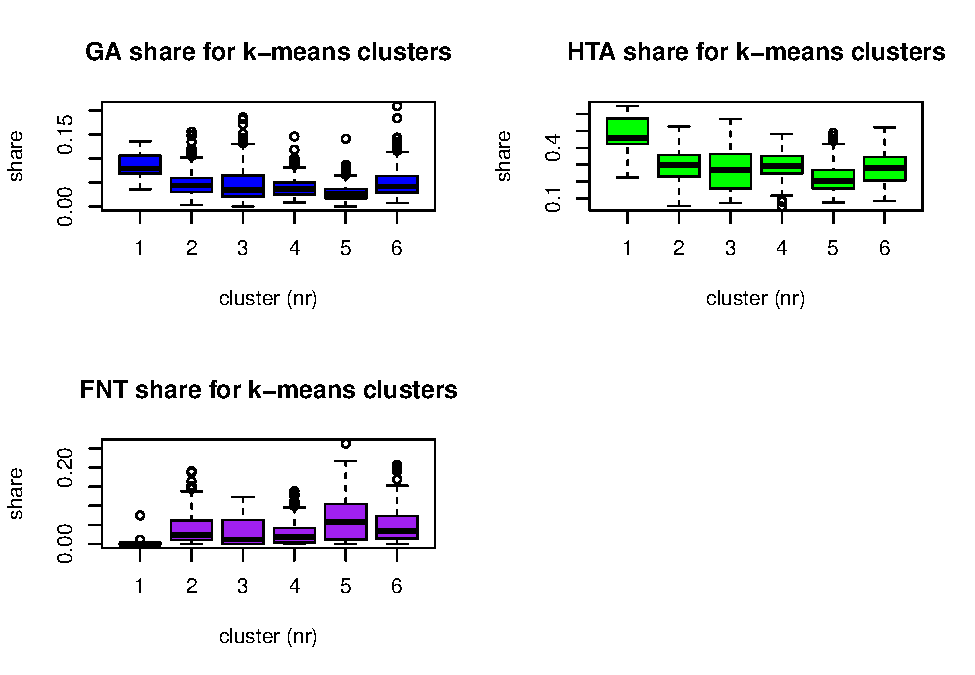
\includegraphics{Influence_factors_files/figure-latex/3.14_share_distr_cl_munic-1.pdf}

\hypertarget{cluster-analysis-on-the-level-of-the-cantons}{%
\subsection{Cluster analysis on the level of the
cantons}\label{cluster-analysis-on-the-level-of-the-cantons}}

\hypertarget{loading-and-normalizing-data}{%
\subsubsection{Loading and normalizing
data}\label{loading-and-normalizing-data}}

\begin{Shaded}
\begin{Highlighting}[]
\CommentTok{\# Loading data}
\NormalTok{d.cant.share }\OtherTok{\textless{}{-}} \FunctionTok{read.csv}\NormalTok{(}\StringTok{"../Data/Cleaned/inf\_fac\_cant\_share.csv"}\NormalTok{)}
\CommentTok{\# print(colnames(d.cant.share))}

\CommentTok{\# select columns to normalize}
\NormalTok{columns }\OtherTok{\textless{}{-}} \FunctionTok{c}\NormalTok{(}\StringTok{"PT\_dist\_medium"}\NormalTok{, }\StringTok{"PT\_time\_medium"}\NormalTok{, }\StringTok{"PT\_dist\_big"}\NormalTok{, }\StringTok{"PT\_time\_big"}\NormalTok{,}
             \StringTok{"str\_dist\_medium"}\NormalTok{, }\StringTok{"str\_time\_medium"}\NormalTok{ ,}\StringTok{"str\_dist\_big"}\NormalTok{, }\StringTok{"str\_time\_big"}\NormalTok{,}
             \StringTok{"PT\_fact\_big"}\NormalTok{, }\StringTok{"PT\_fact\_medium"}\NormalTok{, }\StringTok{"single\_share"}\NormalTok{, }\StringTok{"married\_share"}\NormalTok{, }
             \StringTok{"widowed\_share"}\NormalTok{, }\StringTok{"divorced\_share"}\NormalTok{, }\StringTok{"GA\_share"}\NormalTok{, }\StringTok{"HTA\_share"}\NormalTok{,}
             \StringTok{"FNT\_share"}\NormalTok{, }\StringTok{"age0\_20\_share"}\NormalTok{, }\StringTok{"age20\_40\_share"}\NormalTok{, }\StringTok{"age40\_60\_share"}\NormalTok{,}
             \StringTok{"age60.\_share"}\NormalTok{, }\StringTok{"birth\_munic\_share"}\NormalTok{, }\StringTok{"birth\_cant\_share"}\NormalTok{, }
             \StringTok{"birth\_CH\_share"}\NormalTok{, }\StringTok{"birth\_notCH\_share"}\NormalTok{, }\StringTok{"male\_share"}\NormalTok{, }\StringTok{"female\_share"}\NormalTok{,}
             \StringTok{"resid\_0\_1y\_share"}\NormalTok{, }\StringTok{"resid\_1\_5y\_share"}\NormalTok{, }\StringTok{"resid\_6\_10y\_share"}\NormalTok{, }
             \StringTok{"resid\_10.y\_share"}\NormalTok{, }\StringTok{"hh\_1\_share"}\NormalTok{, }\StringTok{"hh\_2\_share"}\NormalTok{, }\StringTok{"hh\_3\_5\_share"}\NormalTok{, }
             \StringTok{"hh\_6.\_share"}\NormalTok{, }\StringTok{"bus\_stops\_per\_pop"}\NormalTok{, }\StringTok{"other\_stops\_per\_pop"}\NormalTok{, }
             \StringTok{"train\_stops\_per\_pop"}\NormalTok{, }\StringTok{"bus\_stat\_per\_1000"}\NormalTok{, }\StringTok{"other\_stat\_per\_1000"}\NormalTok{,}
             \StringTok{"train\_stat\_per\_1000"}\NormalTok{, }\StringTok{"comb\_car\_per\_1000"}\NormalTok{, }\StringTok{"el\_car\_per\_1000"}\NormalTok{)}

\CommentTok{\# normalize data}
\NormalTok{d.cant.norm.share }\OtherTok{\textless{}{-}}\NormalTok{ d.cant.share}
\NormalTok{d.cant.norm.share[columns] }\OtherTok{\textless{}{-}} \FunctionTok{scale}\NormalTok{(d.cant.norm.share[columns])}
\end{Highlighting}
\end{Shaded}

\begin{Shaded}
\begin{Highlighting}[]
\NormalTok{cl.an.cant.input }\OtherTok{\textless{}{-}}\NormalTok{ d.cant.norm.share[,}\FunctionTok{c}\NormalTok{(}\StringTok{"age0\_20\_share"}\NormalTok{, }\StringTok{"age20\_40\_share"}\NormalTok{,}
                      \StringTok{"birth\_munic\_share"}\NormalTok{, }\StringTok{"birth\_cant\_share"}\NormalTok{, }\StringTok{"birth\_CH\_share"}\NormalTok{,}
                      \StringTok{"male\_share"}\NormalTok{, }\StringTok{"resid\_6\_10y\_share"}\NormalTok{, }\StringTok{"hh\_1\_share"}\NormalTok{, }\StringTok{"hh\_2\_share"}\NormalTok{,}
                      \StringTok{"hh\_3\_5\_share"}\NormalTok{, }\StringTok{"PT\_time\_medium"}\NormalTok{, }\StringTok{"PT\_time\_big"}\NormalTok{, }\StringTok{"train\_stops\_per\_pop"}\NormalTok{,}
                      \StringTok{"bus\_stat\_per\_1000"}\NormalTok{, }\StringTok{"other\_stat\_per\_1000"}\NormalTok{, }\StringTok{"comb\_car\_per\_1000"}\NormalTok{,}
                      \StringTok{"el\_car\_per\_1000"}\NormalTok{, }\StringTok{"PT\_fact\_big"}\NormalTok{, }\StringTok{"single\_share"}\NormalTok{, }\StringTok{"married\_share"}\NormalTok{,}
                      \StringTok{"other\_stops\_per\_pop"}\NormalTok{, }\StringTok{"train\_stat\_per\_1000"}\NormalTok{, }\StringTok{"PT\_fact\_medium"}\NormalTok{,}
                      \StringTok{"bus\_stops\_per\_pop"}\NormalTok{)]}

\CommentTok{\# set row names according to canton labels}
\FunctionTok{row.names}\NormalTok{(cl.an.cant.input) }\OtherTok{\textless{}{-}}\NormalTok{ d.cant.norm.share}\SpecialCharTok{$}\NormalTok{canton}
\end{Highlighting}
\end{Shaded}

\hypertarget{preparation-of-clustering-1}{%
\subsubsection{Preparation of
clustering}\label{preparation-of-clustering-1}}

\begin{Shaded}
\begin{Highlighting}[]
\CommentTok{\# distance matrix}
\NormalTok{dp\_cant }\OtherTok{\textless{}{-}} \FunctionTok{dist}\NormalTok{(cl.an.cant.input)}

\CommentTok{\# Principal components}
\NormalTok{PC.inf.fac.cant }\OtherTok{\textless{}{-}} \FunctionTok{princomp}\NormalTok{(cl.an.cant.input) }\CommentTok{\# without language}
\FunctionTok{summary}\NormalTok{(PC.inf.fac.cant, }\AttributeTok{loadings =} \ConstantTok{FALSE}\NormalTok{)}
\end{Highlighting}
\end{Shaded}

\begin{verbatim}
## Importance of components:
##                          Comp.1    Comp.2    Comp.3     Comp.4     Comp.5
## Standard deviation     2.512686 2.0634228 1.7028587 1.48489202 1.28197927
## Proportion of Variance 0.273589 0.1845009 0.1256549 0.09554585 0.07121707
## Cumulative Proportion  0.273589 0.4580899 0.5837448 0.67929064 0.75050771
##                            Comp.6     Comp.7     Comp.8     Comp.9    Comp.10
## Standard deviation     1.13683275 1.05207005 0.88961478 0.79899706 0.69367111
## Proportion of Variance 0.05600351 0.04796356 0.03429463 0.02766384 0.02085112
## Cumulative Proportion  0.80651122 0.85447478 0.88876941 0.91643324 0.93728436
##                           Comp.11    Comp.12    Comp.13    Comp.14     Comp.15
## Standard deviation     0.62107403 0.55136949 0.54185768 0.37957123 0.307832714
## Proportion of Variance 0.01671509 0.01317369 0.01272309 0.00624322 0.004106309
## Cumulative Proportion  0.95399946 0.96717315 0.97989624 0.98613946 0.990245768
##                            Comp.16     Comp.17     Comp.18      Comp.19
## Standard deviation     0.289400362 0.241991072 0.228073617 0.1212260569
## Proportion of Variance 0.003629278 0.002537586 0.002254095 0.0006368161
## Cumulative Proportion  0.993875046 0.996412632 0.998666727 0.9993035430
##                             Comp.20      Comp.21      Comp.22      Comp.23
## Standard deviation     0.0958560874 0.0700329322 4.019855e-02 1.828023e-02
## Proportion of Variance 0.0003981635 0.0002125332 7.002335e-05 1.448056e-05
## Cumulative Proportion  0.9997017065 0.9999142397 9.999843e-01 9.999987e-01
##                             Comp.24
## Standard deviation     5.384632e-03
## Proportion of Variance 1.256418e-06
## Cumulative Proportion  1.000000e+00
\end{verbatim}

\begin{Shaded}
\begin{Highlighting}[]
\DocumentationTok{\#\# first 2 PC explain 46\% of variance, 5 PC about 75\% of variance}

\FunctionTok{plot}\NormalTok{(PC.inf.fac.cant, }\AttributeTok{main=}\StringTok{"Principal components: Explained variance per PC"}\NormalTok{)}
\end{Highlighting}
\end{Shaded}

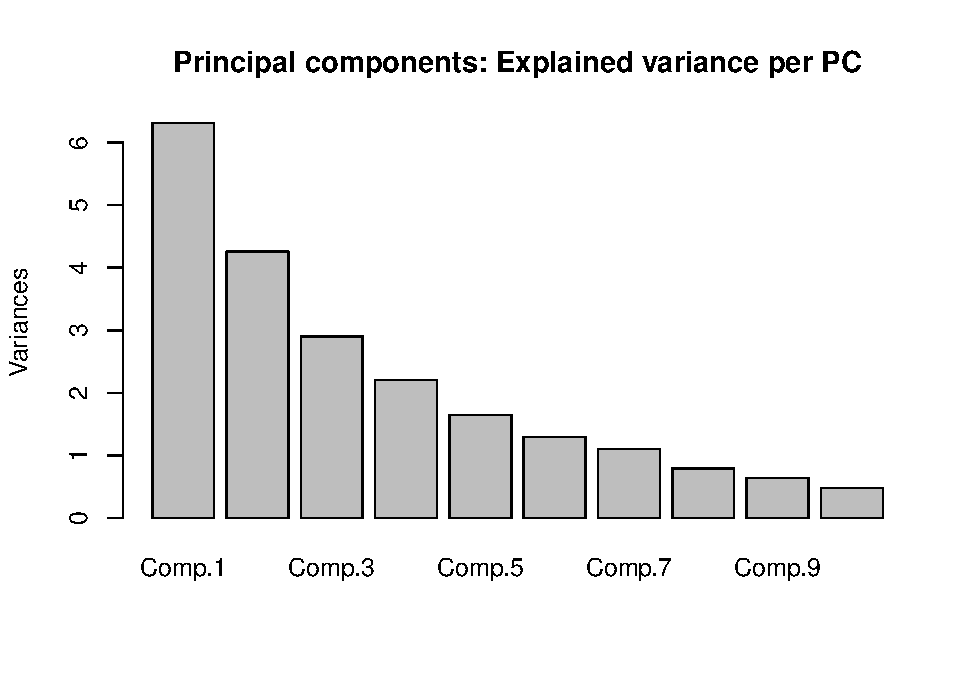
\includegraphics{Influence_factors_files/figure-latex/3.17_ca_data_prep_cant-1.pdf}

\begin{Shaded}
\begin{Highlighting}[]
\CommentTok{\# write two first components out}
\NormalTok{pc.cant }\OtherTok{\textless{}{-}}\NormalTok{ PC.inf.fac.cant}\SpecialCharTok{$}\NormalTok{scores[,}\DecValTok{1}\SpecialCharTok{:}\DecValTok{2}\NormalTok{]}
\end{Highlighting}
\end{Shaded}

\hypertarget{agglomerative-clustering-1}{%
\subsubsection{Agglomerative
Clustering}\label{agglomerative-clustering-1}}

Again here, first the approahc of agglomerative clustering.

\begin{Shaded}
\begin{Highlighting}[]
\DocumentationTok{\#\# Agglomerative clustering with complete linkage}
\NormalTok{cl.cant.inf.fac }\OtherTok{\textless{}{-}} \FunctionTok{hclust}\NormalTok{(dp\_cant, }\AttributeTok{method =} \StringTok{"complete"}\NormalTok{)}

\DocumentationTok{\#\# Show dendrogram}
\FunctionTok{plot}\NormalTok{(cl.cant.inf.fac)}
\FunctionTok{abline}\NormalTok{(}\AttributeTok{h=}\DecValTok{9}\NormalTok{, }\AttributeTok{col=}\StringTok{"red"}\NormalTok{, }\AttributeTok{lty=}\DecValTok{2}\NormalTok{)}
\end{Highlighting}
\end{Shaded}

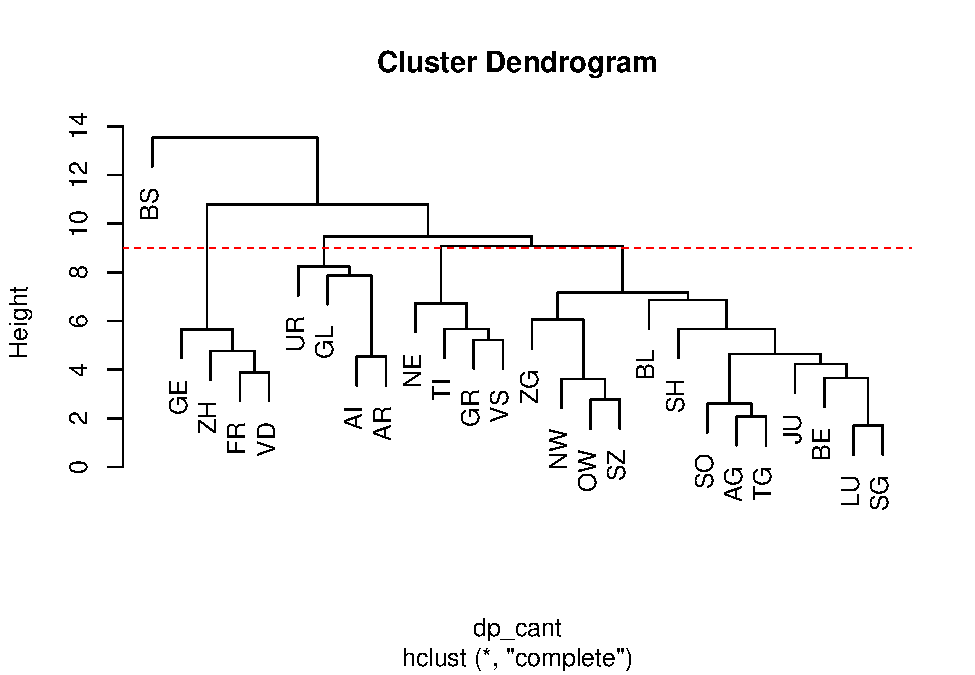
\includegraphics{Influence_factors_files/figure-latex/3.18_aggl_clust1_cant-1.pdf}
Splitting at height 9 would result into 5 different clusters:

\begin{Shaded}
\begin{Highlighting}[]
\DocumentationTok{\#\# Split into groups}
\NormalTok{k }\OtherTok{=} \DecValTok{5} \CommentTok{\# split at height 9 =\textgreater{} 5 groups}
\NormalTok{grps\_cant }\OtherTok{\textless{}{-}} \FunctionTok{cutree}\NormalTok{(cl.cant.inf.fac, }\AttributeTok{k =}\NormalTok{ k) }


\CommentTok{\# plotting clustering result}
\FunctionTok{plot}\NormalTok{(pc.cant, }\AttributeTok{pch =}\NormalTok{ grps\_cant, }\AttributeTok{col=}\NormalTok{grps\_cant, }\AttributeTok{lwd=}\DecValTok{2}\NormalTok{, }\AttributeTok{type=}\StringTok{"n"}\NormalTok{) }\CommentTok{\# add clustering result}
\FunctionTok{legend}\NormalTok{(}\StringTok{"topleft"}\NormalTok{, }\AttributeTok{legend =} \DecValTok{1}\SpecialCharTok{:}\NormalTok{k, }\AttributeTok{pch =} \DecValTok{1}\SpecialCharTok{:}\NormalTok{k, }\AttributeTok{col=}\DecValTok{1}\SpecialCharTok{:}\NormalTok{k, }\AttributeTok{bty=}\StringTok{"n"}\NormalTok{)}
\FunctionTok{text}\NormalTok{(pc.cant[,}\DecValTok{1}\NormalTok{], pc.cant[,}\DecValTok{2}\NormalTok{], }\AttributeTok{labels=}\NormalTok{d.cant.norm.share}\SpecialCharTok{$}\NormalTok{canton, }\AttributeTok{col=}\NormalTok{grps\_cant)}
\end{Highlighting}
\end{Shaded}

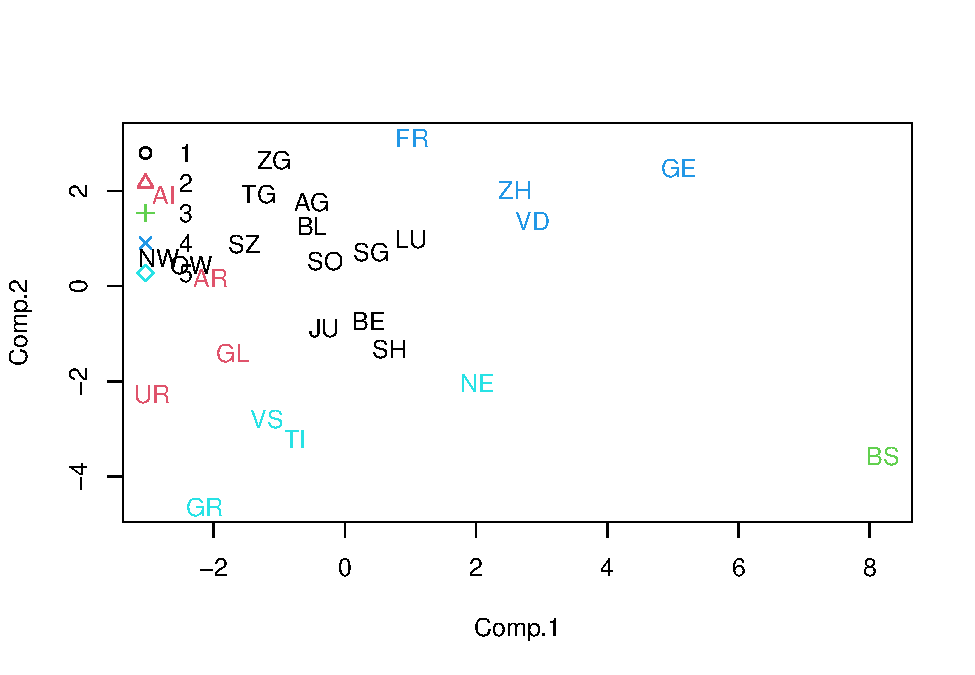
\includegraphics{Influence_factors_files/figure-latex/3.19_aggl_clust2_cant-1.pdf}

\begin{Shaded}
\begin{Highlighting}[]
\DocumentationTok{\#\# Look at means of clusters / centroids}
\FunctionTok{aggregate}\NormalTok{(cl.an.cant.input, }\AttributeTok{by=}\FunctionTok{list}\NormalTok{(}\AttributeTok{cluster=}\NormalTok{grps\_cant), mean)}
\end{Highlighting}
\end{Shaded}

\begin{verbatim}
##   cluster age0_20_share age20_40_share birth_munic_share birth_cant_share
## 1       1     0.0138614     -0.1822481        -0.3682841       0.08717895
## 2       2     0.4144378     -0.2881687         0.6559767      -0.31908379
## 3       3    -1.8788670      2.2386642         3.2214163      -2.74798576
## 4       4     1.1861764      1.3004697        -0.5490215       0.25511454
## 5       5    -1.1759469     -0.9796607         0.2846139       0.46763410
##   birth_CH_share male_share resid_6_10y_share hh_1_share hh_2_share
## 1      0.3774966  0.3582343       -0.18810686 -0.3598379  0.5667078
## 2      0.7110705  0.9401891        0.97896326 -0.6653747  0.5967934
## 3     -0.7726282 -0.7144058       -0.27386238  3.2751432 -1.7734075
## 4     -0.8627021 -0.5274804       -0.09045127  0.0313340 -1.2050783
## 5     -0.8820755 -1.3983685       -0.20869909  0.9847279 -0.7901635
##   hh_3_5_share PT_time_medium PT_time_big train_stops_per_pop bus_stat_per_1000
## 1   -0.0404225    -0.13481799  -0.2200022          -0.2270643        -0.2378860
## 2    0.1957775     0.44008379   0.5086038           1.2067392         0.5583738
## 3   -2.8188930     1.81390328  -1.5713455          -1.6960204        -1.3552683
## 4    1.0909767    -0.36245031  -0.8592068          -0.5177394        -0.8285211
## 5   -0.4506579    -0.09295084   1.4584466           0.4729643         1.3820938
##   other_stat_per_1000 comb_car_per_1000 el_car_per_1000  PT_fact_big
## 1          -0.1582558         0.2739854       0.2746391  0.009474241
## 2           0.8671524         0.4013180      -0.6288553 -0.163032345
## 3          -0.7191758        -3.3862895      -1.1597302  1.240494269
## 4          -0.6355556        -0.8767527       0.2474265  0.999603035
## 5           0.4625286         0.4315545      -0.2212156 -1.177485539
##   single_share married_share other_stops_per_pop train_stat_per_1000
## 1   -0.4382117     0.4579125          -0.2081932          -0.3462886
## 2   -0.3065803     0.6702589           0.5703370           1.3805715
## 3    2.1289961    -2.5420811          -0.3901727          -1.4640645
## 4    1.5082327    -1.2237077          -0.5246842          -0.6039516
## 5   -0.3097136    -0.2992465           0.7285183           0.7148344
##   PT_fact_medium bus_stops_per_pop
## 1    -0.30068441       -0.13768471
## 2     0.43808046       -0.60295192
## 3    -2.12289204        2.34714880
## 4     1.16689793       -0.09192375
## 5    -0.09703105        0.55556376
\end{verbatim}

\hypertarget{k-means-clustering-1}{%
\subsubsection{K-means clustering}\label{k-means-clustering-1}}

Now the second approahc, the k-means clustering

\begin{Shaded}
\begin{Highlighting}[]
\DocumentationTok{\#\#\#\#\#\#\#\#\#\#\#\#\#}
\DocumentationTok{\#\# k{-}means \#\#}
\DocumentationTok{\#\#\#\#\#\#\#\#\#\#\#\#\#}

\DocumentationTok{\#\# Choose number of clusters k with scree plot}
\NormalTok{nr }\OtherTok{\textless{}{-}} \DecValTok{12}
\NormalTok{wss }\OtherTok{\textless{}{-}} \FunctionTok{rep}\NormalTok{(}\DecValTok{0}\NormalTok{, nr)}
\ControlFlowTok{for}\NormalTok{ (i }\ControlFlowTok{in} \DecValTok{1}\SpecialCharTok{:}\NormalTok{nr) wss[i] }\OtherTok{\textless{}{-}} \FunctionTok{sum}\NormalTok{(}\FunctionTok{kmeans}\NormalTok{(cl.an.cant.input, }\AttributeTok{centers =}\NormalTok{ i, }\AttributeTok{nstart =} \DecValTok{20}\NormalTok{)}\SpecialCharTok{$}\NormalTok{withinss)}
\FunctionTok{plot}\NormalTok{(}\DecValTok{1}\SpecialCharTok{:}\NormalTok{nr, wss, }\AttributeTok{type =} \StringTok{"b"}\NormalTok{, }\AttributeTok{xlab =} \StringTok{"Number of groups"}\NormalTok{, }\AttributeTok{ylab =} \StringTok{"Within groups sum of squares"}\NormalTok{) }
\end{Highlighting}
\end{Shaded}

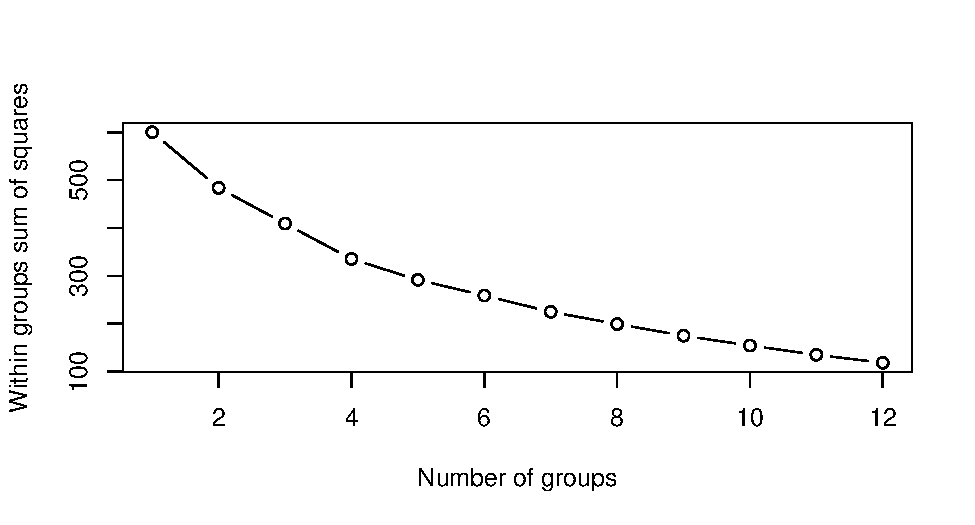
\includegraphics{Influence_factors_files/figure-latex/3.20_kmeans_cant-1.pdf}

\begin{Shaded}
\begin{Highlighting}[]
\DocumentationTok{\#\# good spot at 4, test all from 2 to 10}

\FunctionTok{par}\NormalTok{(}\AttributeTok{mfrow=}\FunctionTok{c}\NormalTok{(}\DecValTok{1}\NormalTok{,}\DecValTok{2}\NormalTok{), }\AttributeTok{mar=}\FunctionTok{c}\NormalTok{(}\DecValTok{5}\NormalTok{,}\DecValTok{4}\NormalTok{,}\DecValTok{4}\NormalTok{,}\DecValTok{2}\NormalTok{), }\AttributeTok{cex.main =} \FloatTok{0.9}\NormalTok{, }\AttributeTok{cex.axis=}\FloatTok{0.9}\NormalTok{)}
\ControlFlowTok{for}\NormalTok{(k }\ControlFlowTok{in} \DecValTok{2}\SpecialCharTok{:}\DecValTok{10}\NormalTok{) \{}

  \DocumentationTok{\#\# k{-}means with 3{-}10 centers}
\NormalTok{  ckm.cant }\OtherTok{\textless{}{-}} \FunctionTok{kmeans}\NormalTok{(cl.an.cant.input, }\AttributeTok{centers =}\NormalTok{ k, }\AttributeTok{nstart =} \DecValTok{10}\NormalTok{)}
\NormalTok{  grpsKM.cant }\OtherTok{\textless{}{-}}\NormalTok{ ckm.cant}\SpecialCharTok{$}\NormalTok{cluster}
  
  \DocumentationTok{\#\# Silhouette Plot}
  \FunctionTok{plot}\NormalTok{(}\FunctionTok{silhouette}\NormalTok{(grpsKM.cant, dp\_cant), }
       \AttributeTok{main=}\FunctionTok{paste}\NormalTok{(}\StringTok{"Silhouette plot with"}\NormalTok{, k, }\StringTok{"clusters"}\NormalTok{))}
  
  \DocumentationTok{\#\# visualize in PC 1 \& 2}
  \FunctionTok{plot}\NormalTok{(pc.cant, }\AttributeTok{pch =}\NormalTok{ grpsKM.cant, }\AttributeTok{col=}\NormalTok{grpsKM.cant, }\AttributeTok{lwd=}\DecValTok{2}\NormalTok{, }
       \AttributeTok{main=}\FunctionTok{paste}\NormalTok{(}\StringTok{"k{-}means clustering with"}\NormalTok{, k, }\StringTok{"clusters"}\NormalTok{), }\AttributeTok{type=}\StringTok{"n"}\NormalTok{)}
  \CommentTok{\# legend("topleft", legend = 1:k, pch = 1:k, col=1:k, bty="n")}
  \FunctionTok{text}\NormalTok{(pc.cant[,}\DecValTok{1}\NormalTok{], pc.cant[,}\DecValTok{2}\NormalTok{], }\AttributeTok{labels=}\NormalTok{d.cant.norm.share}\SpecialCharTok{$}\NormalTok{canton, }\AttributeTok{col=}\NormalTok{grpsKM.cant)}
  
\NormalTok{\}}
\end{Highlighting}
\end{Shaded}

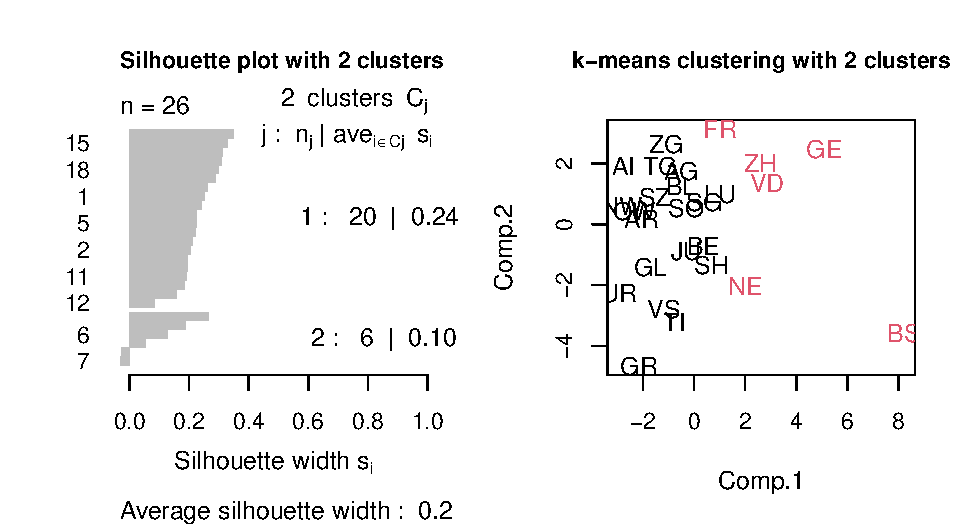
\includegraphics{Influence_factors_files/figure-latex/3.20_kmeans_cant-2.pdf}
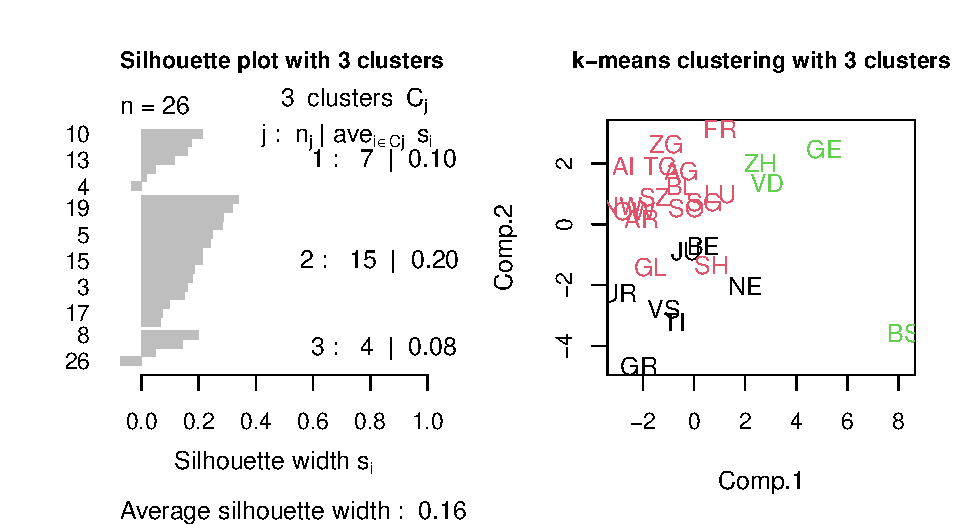
\includegraphics{Influence_factors_files/figure-latex/3.20_kmeans_cant-3.pdf}
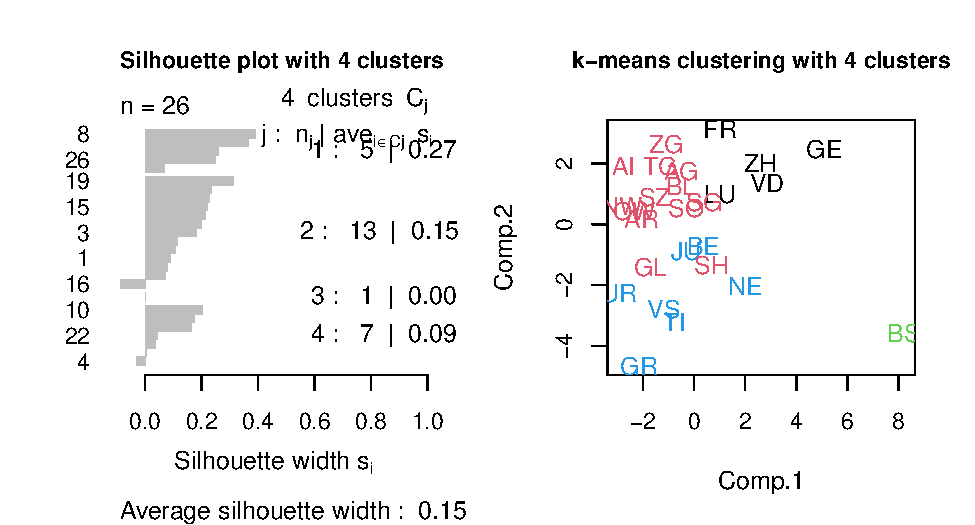
\includegraphics{Influence_factors_files/figure-latex/3.20_kmeans_cant-4.pdf}
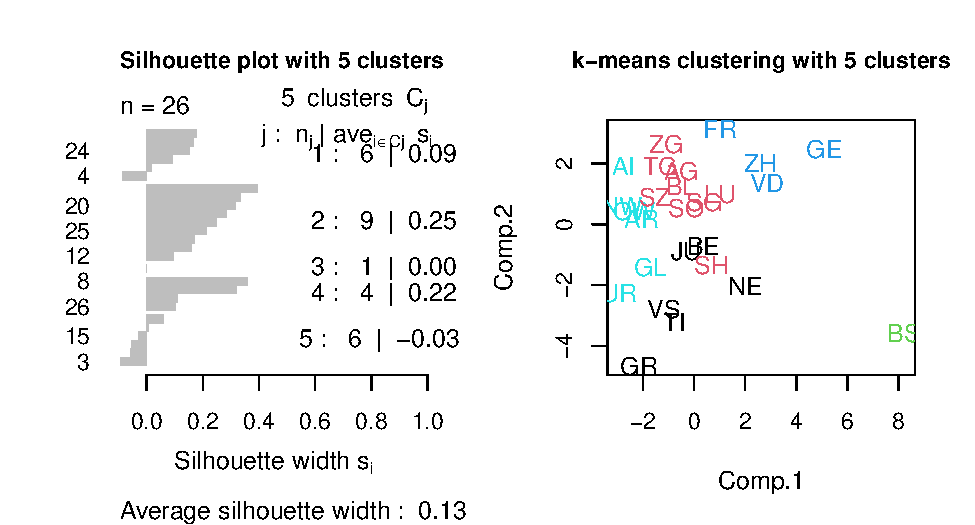
\includegraphics{Influence_factors_files/figure-latex/3.20_kmeans_cant-5.pdf}
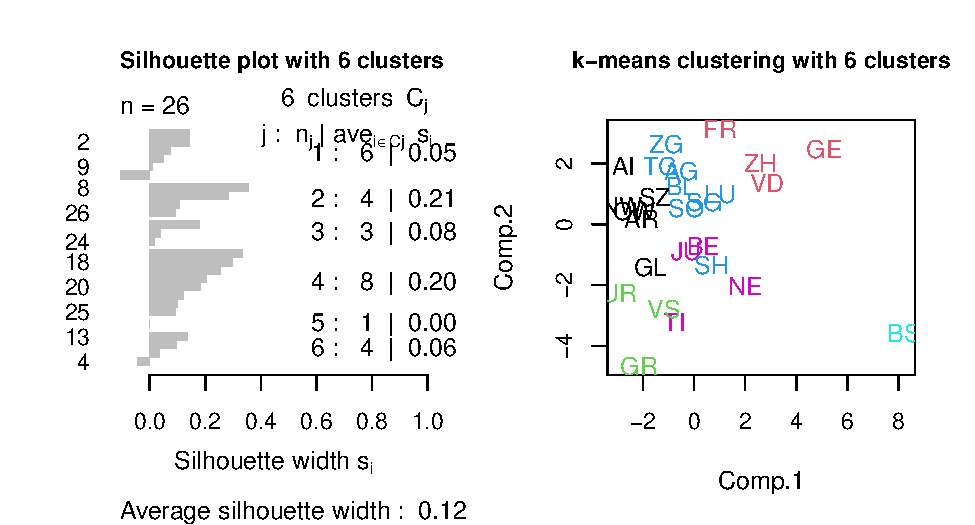
\includegraphics{Influence_factors_files/figure-latex/3.20_kmeans_cant-6.pdf}
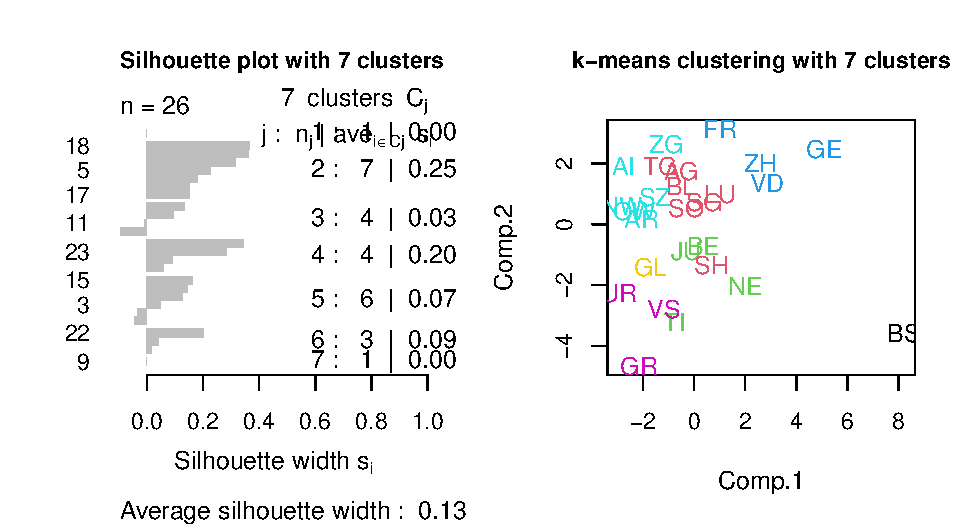
\includegraphics{Influence_factors_files/figure-latex/3.20_kmeans_cant-7.pdf}
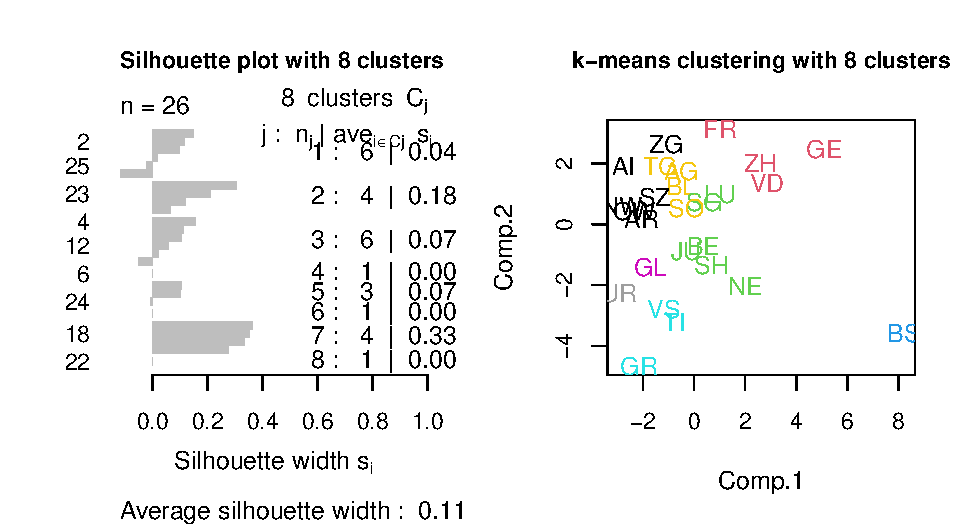
\includegraphics{Influence_factors_files/figure-latex/3.20_kmeans_cant-8.pdf}
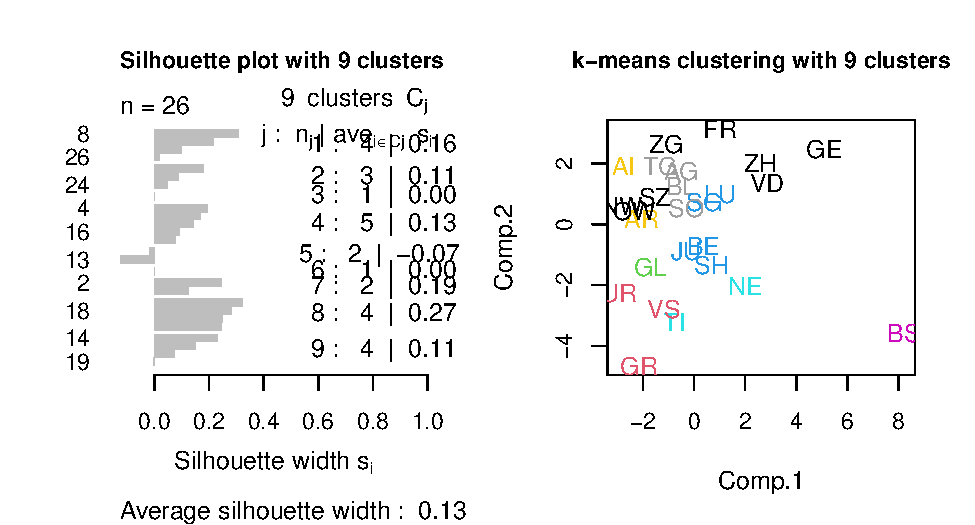
\includegraphics{Influence_factors_files/figure-latex/3.20_kmeans_cant-9.pdf}
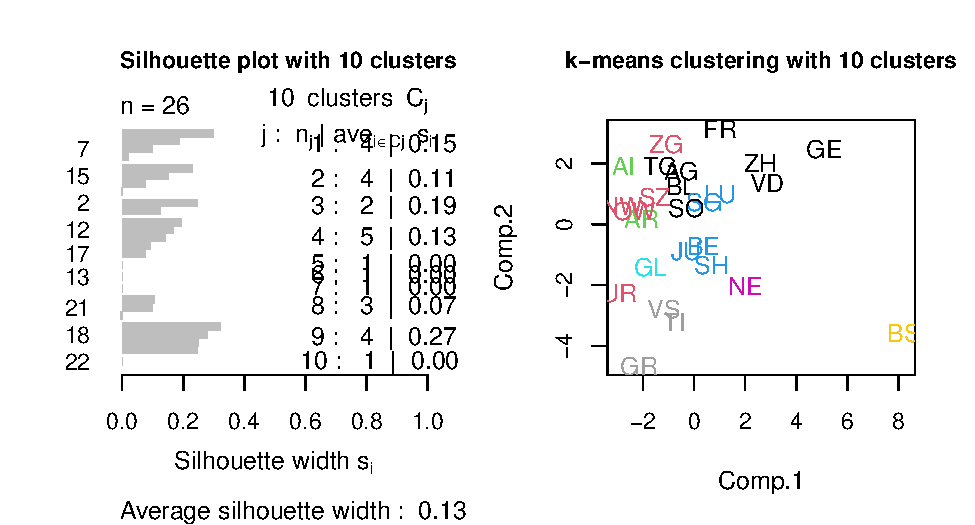
\includegraphics{Influence_factors_files/figure-latex/3.20_kmeans_cant-10.pdf}

\begin{Shaded}
\begin{Highlighting}[]
\DocumentationTok{\#\#\# 4 clusters have the highest average silhouette width!}

\CommentTok{\# k{-}means cluster with k=4}
\NormalTok{ckm4.cant }\OtherTok{\textless{}{-}} \FunctionTok{kmeans}\NormalTok{(cl.an.cant.input, }\AttributeTok{centers =} \DecValTok{4}\NormalTok{, }\AttributeTok{nstart =} \DecValTok{10}\NormalTok{)}
\NormalTok{grpsKM4.cant }\OtherTok{\textless{}{-}}\NormalTok{ ckm4.cant}\SpecialCharTok{$}\NormalTok{cluster}
\end{Highlighting}
\end{Shaded}

Somewhere around 4 clusters seems to be accurate. Going from the
silhouette value, I will take 8 as value.

\hypertarget{dbscan-1}{%
\subsubsection{DBSCAN}\label{dbscan-1}}

\begin{Shaded}
\begin{Highlighting}[]
\DocumentationTok{\#\#\#\#\#\#\#\#\#\#\#\#\#}
\DocumentationTok{\#\# DBSCAN  \#\#}
\DocumentationTok{\#\#\#\#\#\#\#\#\#\#\#\#\#}

\FunctionTok{kNNdistplot}\NormalTok{(cl.an.cant.input, }\AttributeTok{k =} \DecValTok{15}\NormalTok{) }\DocumentationTok{\#\# {-}\textgreater{} eps value = 7.9 (sharp increase)}
\FunctionTok{abline}\NormalTok{(}\AttributeTok{h=}\FloatTok{7.9}\NormalTok{, }\AttributeTok{col =} \StringTok{"red"}\NormalTok{, }\AttributeTok{lty=}\DecValTok{2}\NormalTok{)}
\end{Highlighting}
\end{Shaded}

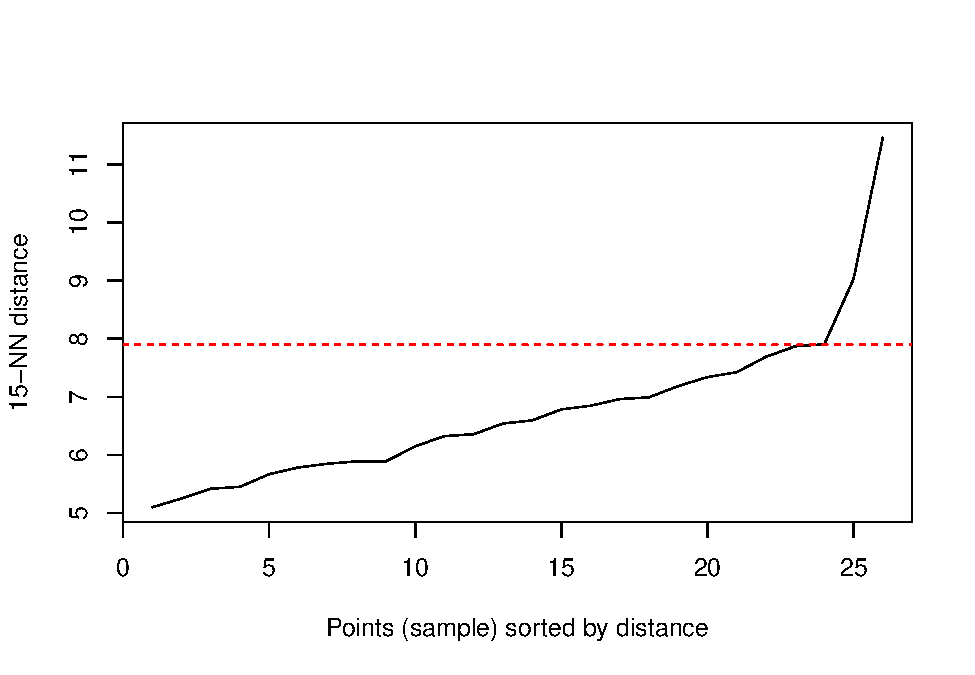
\includegraphics{Influence_factors_files/figure-latex/3.21_dbscan_cant-1.pdf}

\begin{Shaded}
\begin{Highlighting}[]
\CommentTok{\# setting parameters according to minPts = k and eps = sharp increase}

\ControlFlowTok{for}\NormalTok{(i }\ControlFlowTok{in}\NormalTok{ (}\DecValTok{1}\SpecialCharTok{:}\DecValTok{7}\NormalTok{)) \{}
  
  \ControlFlowTok{for}\NormalTok{(j }\ControlFlowTok{in}\NormalTok{ (}\DecValTok{1}\SpecialCharTok{:}\DecValTok{4}\NormalTok{)) \{}

\NormalTok{    dbs.cant }\OtherTok{\textless{}{-}} \FunctionTok{dbscan}\NormalTok{(cl.an.cant.input, }\AttributeTok{eps =}\NormalTok{ i, }\AttributeTok{minPts =}\NormalTok{ j)}

    \FunctionTok{print}\NormalTok{(}\FunctionTok{paste}\NormalTok{(}\StringTok{"minPts:"}\NormalTok{, j, }\StringTok{"; eps: "}\NormalTok{, i, }\StringTok{"; nr. of clusters: "}\NormalTok{,}
                \FunctionTok{max}\NormalTok{(dbs.cant}\SpecialCharTok{$}\NormalTok{cluster))) }\CommentTok{\# 1}
\NormalTok{  \}}

\NormalTok{\}}
\end{Highlighting}
\end{Shaded}

\begin{verbatim}
## [1] "minPts: 1 ; eps:  1 ; nr. of clusters:  26"
## [1] "minPts: 2 ; eps:  1 ; nr. of clusters:  0"
## [1] "minPts: 3 ; eps:  1 ; nr. of clusters:  0"
## [1] "minPts: 4 ; eps:  1 ; nr. of clusters:  0"
## [1] "minPts: 1 ; eps:  2 ; nr. of clusters:  25"
## [1] "minPts: 2 ; eps:  2 ; nr. of clusters:  1"
## [1] "minPts: 3 ; eps:  2 ; nr. of clusters:  0"
## [1] "minPts: 4 ; eps:  2 ; nr. of clusters:  0"
## [1] "minPts: 1 ; eps:  3 ; nr. of clusters:  20"
## [1] "minPts: 2 ; eps:  3 ; nr. of clusters:  1"
## [1] "minPts: 3 ; eps:  3 ; nr. of clusters:  1"
## [1] "minPts: 4 ; eps:  3 ; nr. of clusters:  1"
## [1] "minPts: 1 ; eps:  4 ; nr. of clusters:  12"
## [1] "minPts: 2 ; eps:  4 ; nr. of clusters:  1"
## [1] "minPts: 3 ; eps:  4 ; nr. of clusters:  1"
## [1] "minPts: 4 ; eps:  4 ; nr. of clusters:  1"
## [1] "minPts: 1 ; eps:  5 ; nr. of clusters:  7"
## [1] "minPts: 2 ; eps:  5 ; nr. of clusters:  1"
## [1] "minPts: 3 ; eps:  5 ; nr. of clusters:  1"
## [1] "minPts: 4 ; eps:  5 ; nr. of clusters:  1"
## [1] "minPts: 1 ; eps:  6 ; nr. of clusters:  3"
## [1] "minPts: 2 ; eps:  6 ; nr. of clusters:  1"
## [1] "minPts: 3 ; eps:  6 ; nr. of clusters:  1"
## [1] "minPts: 4 ; eps:  6 ; nr. of clusters:  1"
## [1] "minPts: 1 ; eps:  7 ; nr. of clusters:  2"
## [1] "minPts: 2 ; eps:  7 ; nr. of clusters:  1"
## [1] "minPts: 3 ; eps:  7 ; nr. of clusters:  1"
## [1] "minPts: 4 ; eps:  7 ; nr. of clusters:  1"
\end{verbatim}

\begin{Shaded}
\begin{Highlighting}[]
\CommentTok{\# minPts=1 and eps=5 lead to 7 clusters, eps=6 to 3 clusters. Test these!}

\NormalTok{minPts}\OtherTok{=}\DecValTok{2}
\NormalTok{eps}\OtherTok{=}\DecValTok{5}

\NormalTok{dbs.cant }\OtherTok{\textless{}{-}} \FunctionTok{dbscan}\NormalTok{(cl.an.cant.input, }\AttributeTok{eps =}\NormalTok{ eps, }\AttributeTok{minPts =}\NormalTok{ minPts)}

\FunctionTok{max}\NormalTok{(dbs.cant}\SpecialCharTok{$}\NormalTok{cluster) }\CommentTok{\# 7, look at values}
\end{Highlighting}
\end{Shaded}

\begin{verbatim}
## [1] 1
\end{verbatim}

\begin{Shaded}
\begin{Highlighting}[]
\DocumentationTok{\#\# plot on PC 1 \& 2}
\FunctionTok{plot}\NormalTok{(pc.cant, }\AttributeTok{pch =}\NormalTok{ dbs.cant}\SpecialCharTok{$}\NormalTok{cluster}\SpecialCharTok{+}\DecValTok{1}\NormalTok{, }\AttributeTok{col =}\NormalTok{ dbs.cant}\SpecialCharTok{$}\NormalTok{cluster}\SpecialCharTok{+}\DecValTok{1}\NormalTok{, }\AttributeTok{type=}\StringTok{"n"}\NormalTok{)}
\FunctionTok{legend}\NormalTok{(}\StringTok{"topleft"}\NormalTok{, }\AttributeTok{legend =} \DecValTok{0}\SpecialCharTok{:}\FunctionTok{max}\NormalTok{(dbs.cant}\SpecialCharTok{$}\NormalTok{cluster), }\AttributeTok{pch =} \DecValTok{1}\SpecialCharTok{:}\NormalTok{(}\FunctionTok{max}\NormalTok{(dbs.cant}\SpecialCharTok{$}\NormalTok{cluster)}\SpecialCharTok{+}\DecValTok{1}\NormalTok{),}
       \AttributeTok{col =} \DecValTok{1}\SpecialCharTok{:}\NormalTok{(}\FunctionTok{max}\NormalTok{(dbs.cant}\SpecialCharTok{$}\NormalTok{cluster)}\SpecialCharTok{+}\DecValTok{1}\NormalTok{))}
\FunctionTok{text}\NormalTok{(pc.cant[,}\DecValTok{1}\NormalTok{], pc.cant[,}\DecValTok{2}\NormalTok{], }\AttributeTok{labels=}\NormalTok{d.cant.norm.share}\SpecialCharTok{$}\NormalTok{canton, }\AttributeTok{col=}\NormalTok{dbs.cant}\SpecialCharTok{$}\NormalTok{cluster}\SpecialCharTok{+}\DecValTok{1}\NormalTok{)}
\end{Highlighting}
\end{Shaded}

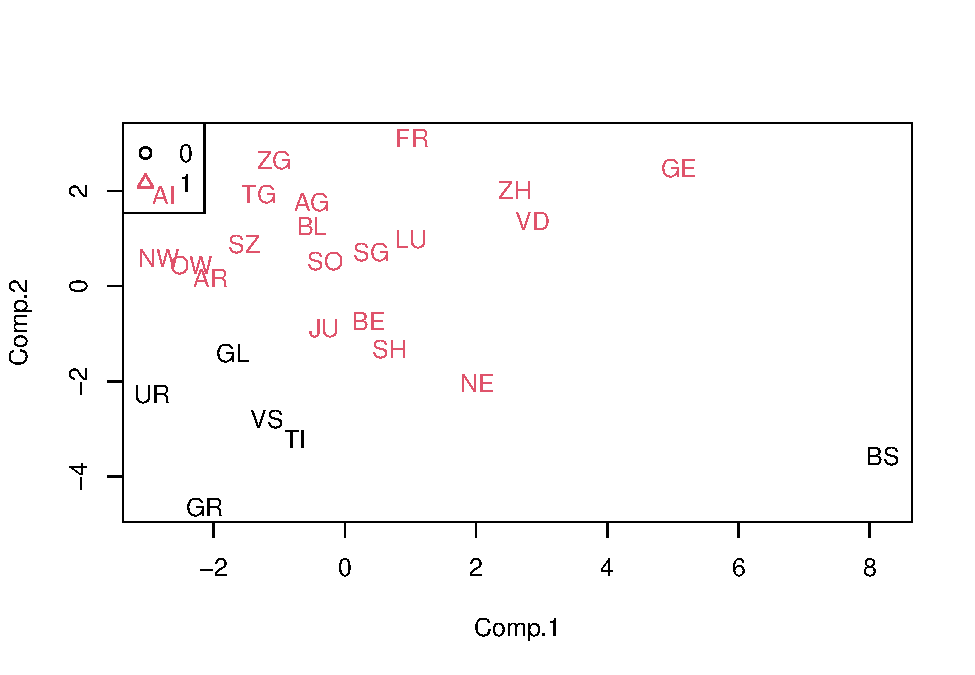
\includegraphics{Influence_factors_files/figure-latex/3.21_dbscan_cant-2.pdf}

\begin{Shaded}
\begin{Highlighting}[]
\FunctionTok{table}\NormalTok{(dbs.cant}\SpecialCharTok{$}\NormalTok{cluster)}
\end{Highlighting}
\end{Shaded}

\begin{verbatim}
## 
##  0  1 
##  6 20
\end{verbatim}

It is always the case that either only one cluster is created, or
individual cantons then form their own cluster. It can be concluded from
this that no suitable cluster analysis is possible with DBSCAN.

\hypertarget{gaussian-mixture-model-1}{%
\subsubsection{Gaussian mixture model}\label{gaussian-mixture-model-1}}

\begin{Shaded}
\begin{Highlighting}[]
\DocumentationTok{\#\# Gaussian Mixture Models}

\NormalTok{mc.cant }\OtherTok{\textless{}{-}} \FunctionTok{Mclust}\NormalTok{(cl.an.cant.input)}
\FunctionTok{table}\NormalTok{(mc.cant}\SpecialCharTok{$}\NormalTok{classification)}
\end{Highlighting}
\end{Shaded}

\begin{verbatim}
## 
##  1  2 
## 25  1
\end{verbatim}

This two classes built are not very useful.

\hypertarget{comparison-of-different-approaches-1}{%
\subsubsection{Comparison of different
approaches}\label{comparison-of-different-approaches-1}}

\begin{Shaded}
\begin{Highlighting}[]
\FunctionTok{par}\NormalTok{(}\AttributeTok{mfrow=}\FunctionTok{c}\NormalTok{(}\DecValTok{1}\NormalTok{,}\DecValTok{2}\NormalTok{), }\AttributeTok{mar=}\FunctionTok{c}\NormalTok{(}\DecValTok{2}\NormalTok{,}\DecValTok{2}\NormalTok{,}\FloatTok{1.5}\NormalTok{,}\DecValTok{1}\NormalTok{))}

\CommentTok{\# K{-}means with 4 clusters}
\FunctionTok{plot}\NormalTok{(pc.cant, }\AttributeTok{pch =}\NormalTok{ grpsKM4.cant, }\AttributeTok{col=}\NormalTok{grpsKM4.cant, }\AttributeTok{main=}\StringTok{"K{-}means (4 clusters)"}\NormalTok{, }\AttributeTok{type=}\StringTok{"n"}\NormalTok{)}
\FunctionTok{legend}\NormalTok{(}\StringTok{"topright"}\NormalTok{, }\AttributeTok{legend =} \DecValTok{1}\SpecialCharTok{:}\DecValTok{4}\NormalTok{, }\AttributeTok{pch =} \DecValTok{1}\SpecialCharTok{:}\DecValTok{4}\NormalTok{, }\AttributeTok{col=}\DecValTok{1}\SpecialCharTok{:}\DecValTok{4}\NormalTok{, }\AttributeTok{bty=}\StringTok{"n"}\NormalTok{, }\AttributeTok{cex=}\FloatTok{0.8}\NormalTok{)}
\FunctionTok{text}\NormalTok{(pc.cant[,}\DecValTok{1}\NormalTok{], pc.cant[,}\DecValTok{2}\NormalTok{], }\AttributeTok{labels=}\NormalTok{d.cant.norm.share}\SpecialCharTok{$}\NormalTok{canton, }\AttributeTok{col=}\NormalTok{grpsKM4.cant)}

\CommentTok{\# Agglomerative clustering}
\FunctionTok{plot}\NormalTok{(pc.cant, }\AttributeTok{pch =}\NormalTok{ grps\_cant, }\AttributeTok{col=}\NormalTok{grps\_cant, }
     \AttributeTok{main=}\StringTok{"Agglomerative clustering (5 clusters)"}\NormalTok{, }\AttributeTok{type=}\StringTok{"n"}\NormalTok{) }\CommentTok{\# add clustering result}
\FunctionTok{legend}\NormalTok{(}\StringTok{"topright"}\NormalTok{, }\AttributeTok{legend =} \DecValTok{1}\SpecialCharTok{:}\DecValTok{5}\NormalTok{, }\AttributeTok{pch =} \DecValTok{1}\SpecialCharTok{:}\DecValTok{5}\NormalTok{, }\AttributeTok{col=}\DecValTok{1}\SpecialCharTok{:}\DecValTok{5}\NormalTok{, }\AttributeTok{bty=}\StringTok{"n"}\NormalTok{, }\AttributeTok{cex=}\FloatTok{0.8}\NormalTok{)}
\FunctionTok{text}\NormalTok{(pc.cant[,}\DecValTok{1}\NormalTok{], pc.cant[,}\DecValTok{2}\NormalTok{], }\AttributeTok{labels=}\NormalTok{d.cant.norm.share}\SpecialCharTok{$}\NormalTok{canton, }\AttributeTok{col=}\NormalTok{grps\_cant)}
\end{Highlighting}
\end{Shaded}

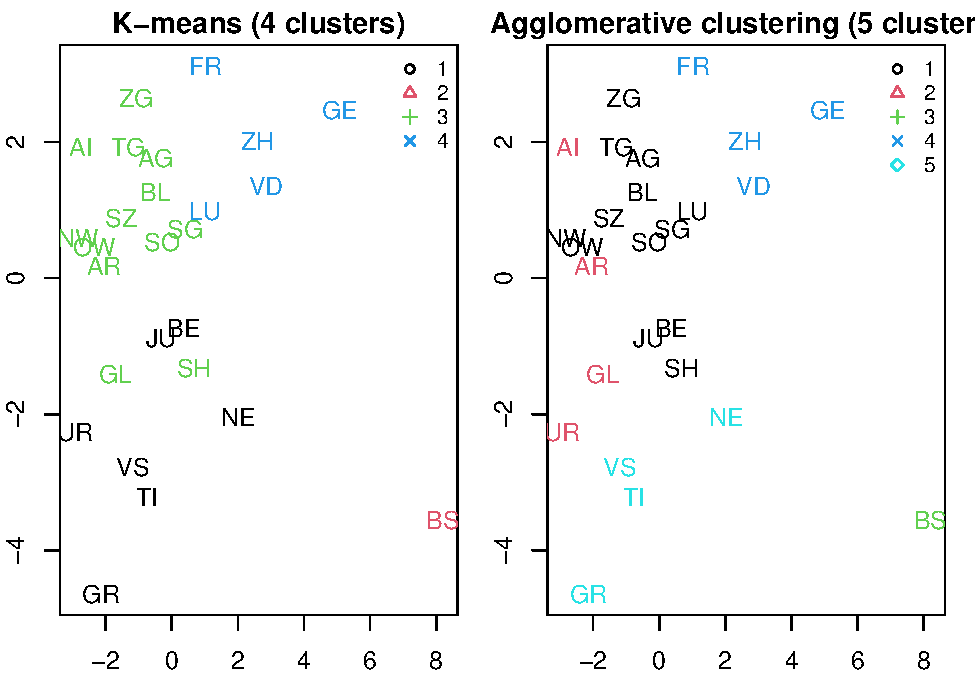
\includegraphics{Influence_factors_files/figure-latex/3.23_ca_comparison1_cant-1.pdf}

\begin{Shaded}
\begin{Highlighting}[]
\DocumentationTok{\#\# Silhouette values \#\#}

\CommentTok{\# Silhouette plot from package "cluster"}
\FunctionTok{par}\NormalTok{(}\AttributeTok{mfrow=}\FunctionTok{c}\NormalTok{(}\DecValTok{1}\NormalTok{,}\DecValTok{2}\NormalTok{), }\AttributeTok{mar=}\FunctionTok{c}\NormalTok{(}\DecValTok{5}\NormalTok{,}\DecValTok{4}\NormalTok{,}\DecValTok{4}\NormalTok{,}\DecValTok{2}\NormalTok{))}
 
\FunctionTok{plot}\NormalTok{(}\FunctionTok{silhouette}\NormalTok{(grpsKM4.cant, dp\_cant), }\AttributeTok{main=}\StringTok{"k{-}means Clustering (k=4)"}\NormalTok{)}
\FunctionTok{plot}\NormalTok{(}\FunctionTok{silhouette}\NormalTok{(grps\_cant, dp\_cant), }\AttributeTok{main=}\StringTok{"Agglomerative clustering"}\NormalTok{)}
\end{Highlighting}
\end{Shaded}

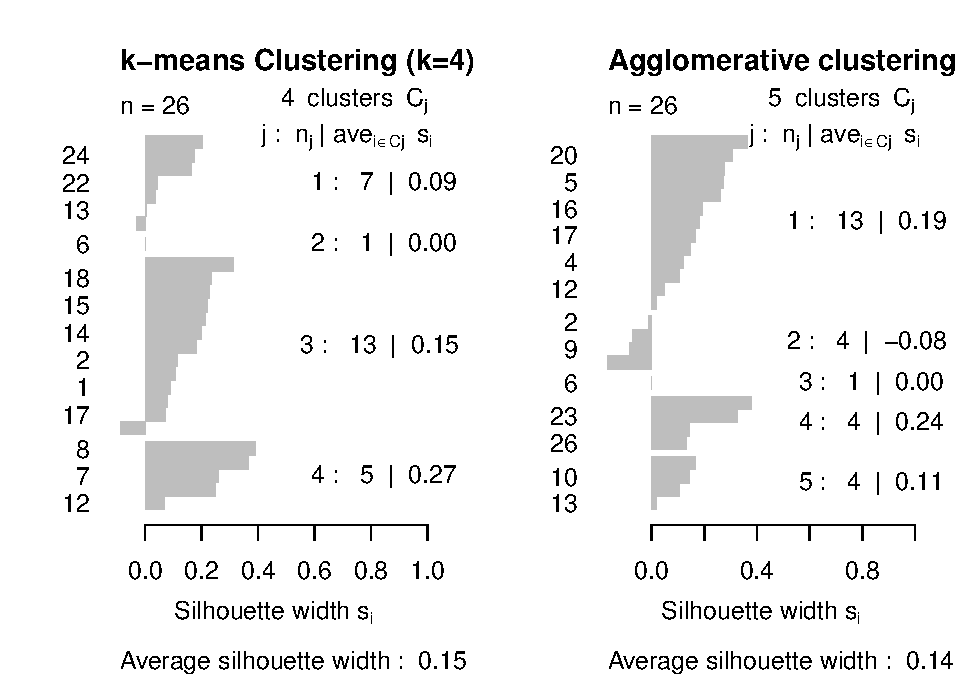
\includegraphics{Influence_factors_files/figure-latex/3.24_ca_comparison2_cant-1.pdf}
The k-means clustering looks slightly better, with no group having a
negative average silhouette width!

\hypertarget{exporting-enriched-data-1}{%
\subsubsection{Exporting enriched
data}\label{exporting-enriched-data-1}}

The generated clusters can now be written into a table together with the
relevant influencing factors, which can then be used for the
distribution of shares and graphical analysis with Tableau.

\begin{Shaded}
\begin{Highlighting}[]
\NormalTok{d.cant.share.clust }\OtherTok{\textless{}{-}}\NormalTok{ d.cant.share}
\NormalTok{d.cant.share.clust[}\StringTok{"k\_cluster"}\NormalTok{] }\OtherTok{=}\NormalTok{ grpsKM4.cant}
\NormalTok{d.cant.share.clust[}\StringTok{"aggl\_cluster"}\NormalTok{] }\OtherTok{=}\NormalTok{ grps\_cant}

\CommentTok{\# categorical data}
\NormalTok{d.cant.share.clust}\SpecialCharTok{$}\NormalTok{k\_cluster}\OtherTok{\textless{}{-}}\FunctionTok{as.factor}\NormalTok{(d.cant.share.clust}\SpecialCharTok{$}\NormalTok{k\_cluster)}
\NormalTok{d.cant.share.clust}\SpecialCharTok{$}\NormalTok{aggl\_cluster}\OtherTok{\textless{}{-}}\FunctionTok{as.factor}\NormalTok{(d.cant.share.clust}\SpecialCharTok{$}\NormalTok{aggl\_cluster)}

\FunctionTok{write.csv}\NormalTok{(d.cant.share.clust, }\AttributeTok{file=}\StringTok{"cant\_influence\_factors\_with\_CA.csv"}\NormalTok{)}
\end{Highlighting}
\end{Shaded}

\hypertarget{share-distribution-of-ga-hta-and-fnt-for-clusters-1}{%
\subsubsection{Share distribution of GA, HTA and FNT for
clusters}\label{share-distribution-of-ga-hta-and-fnt-for-clusters-1}}

\begin{Shaded}
\begin{Highlighting}[]
\FunctionTok{par}\NormalTok{(}\AttributeTok{mfrow=}\FunctionTok{c}\NormalTok{(}\DecValTok{2}\NormalTok{,}\DecValTok{2}\NormalTok{))}
\FunctionTok{boxplot}\NormalTok{(d.cant.share.clust}\SpecialCharTok{$}\NormalTok{GA\_share }\SpecialCharTok{\textasciitilde{}}\NormalTok{ d.cant.share.clust}\SpecialCharTok{$}\NormalTok{aggl\_cluster, }\AttributeTok{col=}\StringTok{"blue"}\NormalTok{,}
        \AttributeTok{main =} \StringTok{"GA share for agglom. clusters"}\NormalTok{)}
\FunctionTok{boxplot}\NormalTok{(d.cant.share.clust}\SpecialCharTok{$}\NormalTok{HTA\_share }\SpecialCharTok{\textasciitilde{}}\NormalTok{ d.cant.share.clust}\SpecialCharTok{$}\NormalTok{aggl\_cluster, }\AttributeTok{col=}\StringTok{"green"}\NormalTok{,}
        \AttributeTok{main =} \StringTok{"HTA share for agglom. clusters"}\NormalTok{)}
\FunctionTok{boxplot}\NormalTok{(d.cant.share.clust}\SpecialCharTok{$}\NormalTok{FNT\_share }\SpecialCharTok{\textasciitilde{}}\NormalTok{ d.cant.share.clust}\SpecialCharTok{$}\NormalTok{aggl\_cluster, }\AttributeTok{col=}\StringTok{"purple"}\NormalTok{,}
        \AttributeTok{main =} \StringTok{"FNT share for agglom. clusters"}\NormalTok{)}
\end{Highlighting}
\end{Shaded}

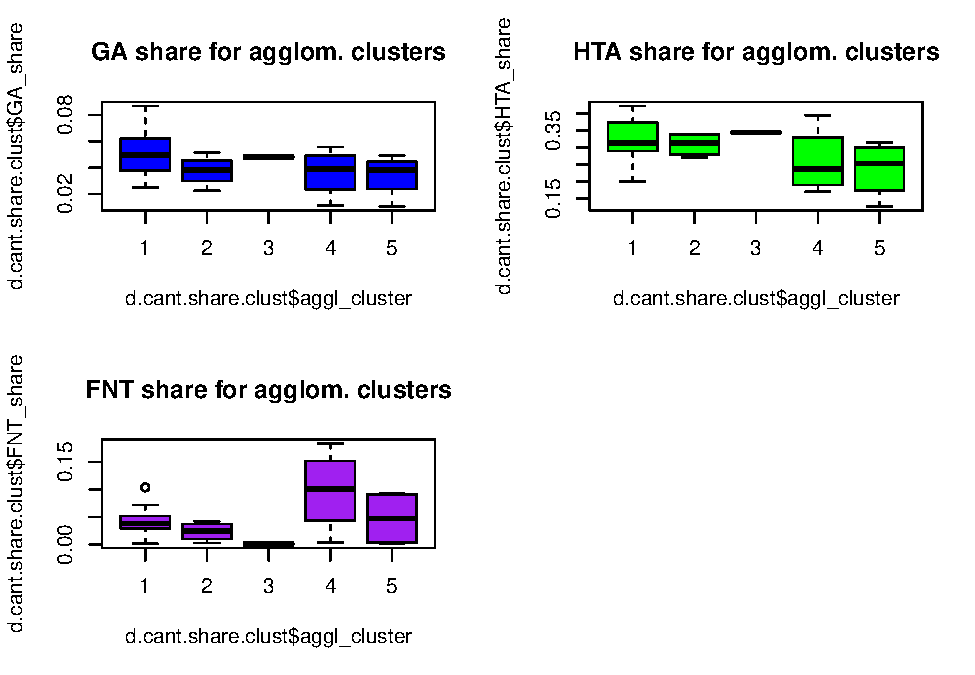
\includegraphics{Influence_factors_files/figure-latex/3.26_share_distr_aggCl_cant-1.pdf}

\begin{Shaded}
\begin{Highlighting}[]
\FunctionTok{par}\NormalTok{(}\AttributeTok{mfrow=}\FunctionTok{c}\NormalTok{(}\DecValTok{2}\NormalTok{,}\DecValTok{2}\NormalTok{))}
\FunctionTok{boxplot}\NormalTok{(d.cant.share.clust}\SpecialCharTok{$}\NormalTok{GA\_share }\SpecialCharTok{\textasciitilde{}}\NormalTok{ d.cant.share.clust}\SpecialCharTok{$}\NormalTok{k\_cluster, }\AttributeTok{col=}\StringTok{"blue"}\NormalTok{, }
        \AttributeTok{main =} \StringTok{"GA share for k{-}means clusters"}\NormalTok{)}
\FunctionTok{boxplot}\NormalTok{(d.cant.share.clust}\SpecialCharTok{$}\NormalTok{HTA\_share }\SpecialCharTok{\textasciitilde{}}\NormalTok{ d.cant.share.clust}\SpecialCharTok{$}\NormalTok{k\_cluster, }\AttributeTok{col=}\StringTok{"green"}\NormalTok{, }
        \AttributeTok{main =} \StringTok{"HTA share for k{-}means clusters"}\NormalTok{)}
\FunctionTok{boxplot}\NormalTok{(d.cant.share.clust}\SpecialCharTok{$}\NormalTok{FNT\_share }\SpecialCharTok{\textasciitilde{}}\NormalTok{ d.cant.share.clust}\SpecialCharTok{$}\NormalTok{k\_cluster, }\AttributeTok{col=}\StringTok{"purple"}\NormalTok{,}
        \AttributeTok{main =} \StringTok{"FNT share for k{-}means clusters"}\NormalTok{)}
\end{Highlighting}
\end{Shaded}

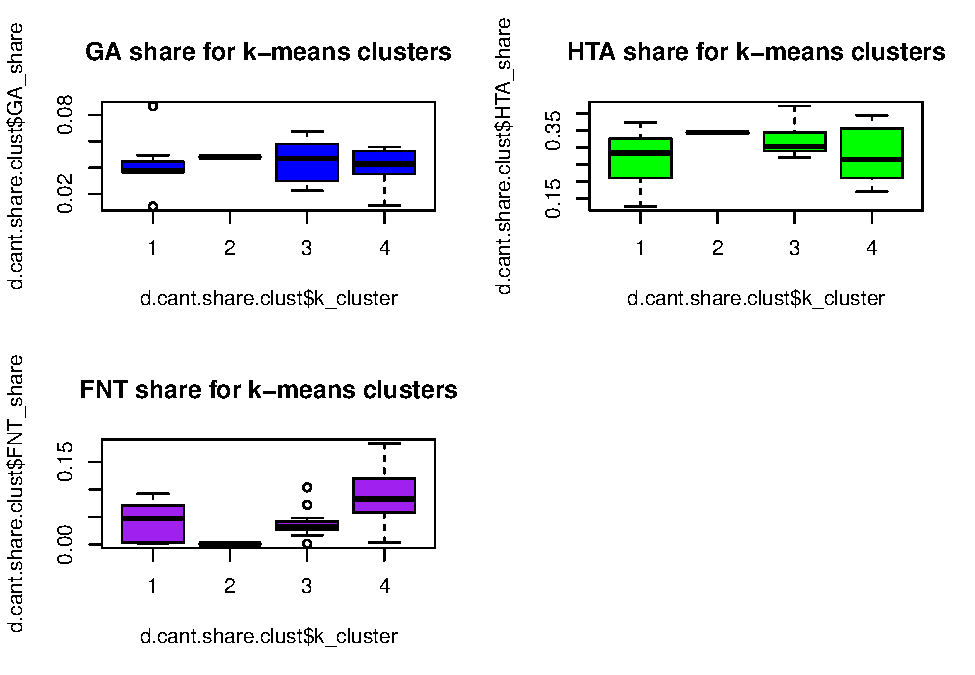
\includegraphics{Influence_factors_files/figure-latex/3.27_share_distr_kmeans_cant-1.pdf}

\end{document}
